\part{\gkchapter{Les unités de la langue}{Les trois composantes du signe linguistique}}\label{sec:2}

\section*{Présentation}

Cette deuxième partie s’intéresse à la délimitation des unités de la langue — les signes linguistiques — selon leur forme, leur combinatoire et leur sens. Le \chapref{sec:2.1} présente rapidement pourquoi nous considérons trois types d’unité. Le \chapref{sec:2.2} présente l’identification des signes linguistiques et plus particulièrement les unités minimales de forme, les morphèmes, et les contrastent avec les unités minimales pour la combinatoire libre, les syntaxèmes. Le \chapref{sec:2.3} présente les unités minimales de sens, les sémantèmes, et les contrastent également avec les syntaxèmes.

\chapter{\gkchapter{Trois types d’unités}{Morphème, syntaxème, sémantème}}\label{sec:2.1}

\section{Introduction}\label{sec:2.1.0}

\begin{quote}
    «~De même que le jeu d’échecs est tout entier dans la combinaison des différentes pièces, de même la langue a le caractère d’un système basé complètement sur l’opposition de ses unités concrètes. On ne peut ni se dispenser de les connaître, ni faire un pas sans recourir à elles ; et pourtant leur délimitation est un problème si délicat qu’on se demande si elles sont réellement données.~» (\citealt{Saussure1916} : 149)
\end{quote}

Notre objectif est d’étudier la structure de la langue. Nous verrons dans la Partie 3 que, contrairement à ce qu’affirme Saussure dans la citation qui précède, on peut en grande partie \textbf{s’abstraire} \textbf{de la question des unités} lorsqu’on définit la structure syntaxique. Ce qui nous intéresse, ce sont les combinaisons entre les unités et non les unités elles-mêmes. Néanmoins, pour pouvoir parler des combinaisons d’unités, il nous faut dire avant un mot des unités. Nous profiterons de cette discussion sur les unités pour montrer que les unités de la langue, que l’on appelle des \textstyleTermes{signes linguistiques}, peuvent être appréhendées selon \textbf{trois points de vue} (morphologique, syntaxique et sémantique) et groupées en ensembles de signes différents selon chacun de ces points de vue. Nous nous attarderons en particulier sur la question des \textbf{unités minimales}. Cette question n’est pas fondamentale pour étudier la structure, mais elle n’est pas inutile non plus et elle a l’avantage de pointer les différences entre morphologie, syntaxe et sémantique.

\section{Double articulation du langage}\label{sec:2.1.1}

\begin{quote}
    «~L’intention et la capacité de signification […] sont constitutives du son articulé ; et on ne peut rien proposer d’autre pour le distinguer d’une part du cri animal et d’autre part du son musical.~» (\citealt{Humboldt1836} : 60)
\end{quote}

Considérons la situation suivante : un acteur vient de faire une performance et vous souhaitez le féliciter, c’est-à-dire lui communiquer le plaisir que vous a procuré sa performance. Vous avez plusieurs moyens à votre disposition et notamment applaudir ou crier «~\textit{Bravo} !~». Chacune de ces deux réalisations possède une \textbf{signification} du type ‘je te félicite’, exprimant que celui qui en fait la réalisation souhaite féliciter celui à qui il l’adresse. Chacune des deux réalisations possède une \textbf{forme} spécifique : l’applaudis\-sement se réalise en frappant les deux mains à plat l’une sur l’autre et «~\textit{Bravo} !~» se réalise en produisant une séquence sonore particulière. Cette association entre une forme et une signification est appelée un \textstyleTermes{signe}. Ces deux actes de communication sont des signes \textstyleTermes{conventionnels~}: la forme de ce signe obéit à une convention que s’est fixée un groupe particulier de personnes et qui leur sert à communiquer. De plus, la relation entre leur signification et leur forme est \textstyleTermes{arbitraire~}: on pourrait tout aussi bien féliciter quelqu’un en levant les bras et en agitant les mains comme le font les sourds en langue des signes, ou bien prononcer une autre séquence sonore, comme le font par exemple les Chinois qui crient «~\textit{Hao} !~» pour communiquer leur appréciation. Inversement l’applaudissement et «~\textit{Bravo} !~» pourraient tout aussi bien signifier autre chose que ‘je te félicite’.

Au delà de leurs points communs, ces deux signes présentent des différences importantes qui tiennent à la \textstyleTermes{double articulation du langage} (voir \encadref{fig:2.1.2} sur l’origine du terme). La \textstyleTermes{première articulation} s’illustre par le fait que le signe \textit{bravo} peut être combiné à d’autres signes pour former des énoncés plus complexes : «~\textit{Bravo pour ton excellente prestation} !~», «~\textit{Alors là, excuse-moi, mais je ne te dis pas bravo pour ce que tu viens de faire.}~». En prenant la question à l’envers, on peut remarquer que la plupart des énoncés de la langue peuvent être décomposés en signes plus élémentaires et que la signification de ces énoncés est la combinaison des significations des signes élémentaires qui les composent. Rien de tel avec l’applaudissement qui ne peut pas être combiné avec un autre signe du même type pour exprimer une signification nouvelle.

La \textstyleTermes{deuxième articulation} tient au fait que la substance sonore des signes d’une langue peut être décomposée en la combinaison d’un tout petit nombre de sons élémentaires. Dans le signifiant de \textit{bravo}, tout locuteur du français reconnaît cinq sons et chacun de ces cinq sons peut être permuté avec un autre son du français pour donner des mots (potentiels) différents du français~\textit{:} \textbf{\textit{t}}\textit{ravo, b}\textbf{\textit{l}}\textit{avo, br}\textbf{\textit{i}}\textit{vo, bra}\textbf{\textit{c}}\textit{o, brav}\textbf{\textit{a}}. Dans toutes les langues du monde, il existe un ensemble fini de quelques dizaines de sons élémentaires qui permettent de construire les signifiants de tous les énoncés de cette langue.

Les unités de première articulation et leurs combinaisons sont les \textstyleTermes{signes linguistiques}. Les unités de deuxième articulation, les \textbf{segments sonores minimaux}, sont les \textstyleTermes{phonèmes}. L’étude des phonèmes en tant que telle est en dehors du champ de cet ouvrage, bien que le \textstyleTermes{système phonologique} d’une langue présente des similitudes structurelles avec le système des signes de la langue et que les outils d’investigation des deux systèmes soient en partie similaires.

\chevalier{Découverte de la double articulation}{%\label{sec:2.1.2}
    L’histoire de la mise en évidence de la double articulation du langage est celle de l’\textbf{invention de l’écriture}. Les étapes de l’invention de l’écriture peuvent être tracées ainsi : d’abord les hommes ont créé des \textstyleTermes{pictogrammes} isolés symbolisant par exemple la fécondité ou la chasse, puis des \textstyleTermes{idéogrammes} associés aux signes linguistiques et combinés pour faire des textes (comme les hiéroglyphes de l’égyptien ancien ou les sinogrammes), puis une \textstyleTermes{écriture syllabaire} avec un symbole par syllabe, et enfin un \textstyleTermes{écriture alphabétique} avec optimalement une lettre par son (comme en phénicien, puis en grec ancien). On peut dire avec certitude que les savants qui ont élaboré les premières écritures alphabétiques il y a plus de 6000 ans avaient compris la double articulation du langage.

    La double articulation du langage a été introduite par Ferdinand de Saussure (\citeyear{Saussure1916} : 26) :

    \begin{quote}
    «~En latin \textit{articulus} signifie «~membre, partie, subdivision dans une suite de choses~» ; en matière de langage, l’articulation peut désigner ou bien la subdivision de la chaîne parlée en syllabes, ou bien la subdivision de la chaîne des significations en unités significatives.~»
    \end{quote}

    On doit le terme de \textstyleTermes{double articulation} à André \citet[13--14]{Martinet1960}:

    \begin{quote}
    «~La \textbf{\textit{première articulation}} du langage est celle selon laquelle tout fait d’expérience à transmettre, tout besoin qu’on désire faire connaître à autrui s’analyse en une suite d’unités douées chacune d’une forme vocale et d’un sens. Si je souffre de douleurs à la tête, je puis manifester la chose par des cris. Ceux-ci peuvent être involontaires ; dans ce cas ils relèvent de la physiologie. Ils peuvent être plus ou moins voulus et destinés à faire connaître mes souffrances à mon entourage. Mais cela ne suffit pas à en faire une communication linguistique. Chaque cri est inanalysable et correspond à l’ensemble, inanalysé, de la sensation douloureuse. Tout autre est la situation si je prononce la phrase \textit{j’ai mal à la tête}. Ici, il n’est aucune des six unités successives \textit{j’, ai, mal, à, la, tête} qui corresponde à ce que ma douleur a de spécifique. Chacune d’entre elle peut se retrouver dans de tout autres contextes pour communiquer d’autres faits d’expérience : \textit{mal}, par exemple, dans \textit{il fait le mal}, et \textit{tête} dans \textit{il s’est mis à leur tête}.~[…] Chacune de ces unités de première articulation présente, nous l’avons vu, un sens et une forme vocale (ou phonique). Elle ne saurait être analysée en unités successives plus petites douées de sens. L’ensemble \textit{tête} veut dire ‘tête’ et l’on ne peut attribuer à \textit{tê-} ou à \textit{{}-te} des sens distincts dont la somme serait équivalente à ‘tête’. Mais la forme vocale est, elle, analysable en une succession d’unités dont chacune contribue à distinguer \textit{tête}, par exemple, d’autres unités comme \textit{bête, tante} ou \textit{terre}. C’est ce qu’on désignera comme la \textbf{\textit{deuxième articulation}} du langage. Dans le cas de \textit{tête}, ces unités sont au nombre de trois ; nous pouvons les représenter au moyen des lettres t e t, placées par convention entre barres obliques, donc /tet/.~»
    \end{quote}

    Si nous reprenons à notre compte la double articulation telle que présentée par Martinet, nous voudrions ajouter une remarque sur ce qui est désigné ici par « cri ». Il est admis aujourd’hui qu’un cri de douleur comme « Aïe ! » est bien un mot du français. Un allemand ne dira pas « \textit{Aïe} ! », mais « \textit{Au!} », (prononcé a-ou) et un anglais «~\textit{Ouch!~}» (prononcé a-outch). Ces signes linguistiques ont une combinatoire beaucoup plus limitée que la plupart des autres signes de la langue (voir la \sectref{sec:5.1.13} sur \textit{Locutifs et interjections}), mais ils n’en sont pas moins analysés de façon comparable et « \textit{Aïe} ! » n’a pas la même signification que « \textit{Aïaïaïe} ! » (prononcé a-ja-jaj)
}
\section{Signifié, syntactique, signifiant}\label{sec:2.1.3}

\begin{styleLivreImportant}
Les unités de première articulation, qui sont les portions de texte porteuses de signification, sont appelées les \textstyleTermes{signes} \textstyleTermes{linguistiques}. (Rappelons que nous désignons par \textit{texte} aussi bien des textes écrits que des productions orales ou gestuelles.) La \textbf{signification} portée par un signe est appelée son \textstyleTermes{signifié}. La \textbf{forme} d’un signe linguistique, en général un segment de texte, est appelée son \textstyleTermes{signifiant}.
\end{styleLivreImportant}

Les signes linguistiques se distinguent des signes de la plupart des autres systèmes sémiotiques par le fait qu’ils peuvent \textbf{se combiner entre eux pour former de nouveaux signes} qui expriment en général des sens qui ne peuvent être exprimés par aucun signe élémentaire. Les signes linguistiques ont donc un potentiel combinatoire qui fait qu’ils possèdent une \textbf{troisième composante}. Cette troisième composante n’est pas réductible aux deux autres. Par exemple, les noms, lorsqu’ils se combinent à un article, déclenchent un accord en genre de cet article : \textbf{\textit{une}} \textit{chaise,} \textbf{\textit{un}} \textit{fauteuil,} \textbf{\textit{un}} \textit{tabouret,} \textbf{\textit{une}} \textit{table}, etc. Rien, ni dans la forme du nom, ni dans son sens, ne permet de prévoir quel sera cet accord — féminin ou masculin. Le locuteur ne peut utiliser correctement un nom en français que s’il a appris cette information en plus du signifiant et du signifié du nom.

\begin{styleLivreImportant}
Le signe linguistique possède donc une troisième composante, appelée son \textstyleTermes{syntactique}, qui contrôle sa \textbf{combinatoire} et qui n’est réductible ni aux propriétés du signifiant, ni à celles du signifié :
\end{styleLivreImportant}

\begin{styleLivreImportant}\bfseries
signe = < signifié, syntactique, signifiant >
\end{styleLivreImportant}

Nous aurons l’occasion de décrire en détail le syntactique des signes. Celui-ci comprend plus d’informations qu’on ne le pense en général. Il comprend d’abord ce qu’on appelle la \textstyleTermes{catégorie syntaxique} du signe. Pour un lexème, il s’agit de la \textstyleTermes{partie du discours} (verbe, nom, adjectif, etc.), mais aussi d’un certain nombre de traits qui contrôlent entre autres la combinatoire flexionnelle (comme le \textstyleTermes{groupe de conjugaison} pour les verbes) ou l’accord (comme le \textstyleTermes{genre} des noms). Le syntactique contient également la \textstyleTermes{valence}, c’est-à-dire la \textbf{liste des compléments régis} par le signe avec le \textstyleTermes{régime} qui leur est imposé, c’est-à-dire les contraintes sur la nature du complément, sa place par rapport au gouverneur et les marques qui doivent l’accompagner (cas, préposition, etc.) (voir les Sections 3.3.10 sur \textit{Distribution et valence} et 3.3.17 sur \textit{Tête interne et rection}). Enfin, le syntactique comprend la description de la \textstyleTermes{cooccurrence lexicale restreinte}, c’est-à-dire toutes les combinaisons qui sont lexicalement contraintes (par exemple le fait que \textit{amoureux} s’intensifie par \textit{follement}, \textit{blessé} par \textit{grièvement}, \textit{malade} par \textit{gravement} et \textit{improbable} par \textit{hautement}) (voir la \sectref{sec:2.3.10} sur \textit{Collocation et choix lié}).

L’étude des signes linguistiques, en raison de leurs trois composantes, relève de trois disciplines différentes : l’étude des signifiés relève de la \textstyleTermes{sémantique}, l’étude du syntactique est le domaine de la \textstyleTermes{syntaxe} et l’étude des signifiants de la \textstyleTermes{morphologie}.

\loupe{Le signe linguistique}{%\label{sec:2.1.4}
    La notion moderne de \textbf{signe linguistique} est généralement attribuée à Saussure (1916 : 98) :\todo[inline]{check "Saussure" against "de Saussure" in whole book}

    \begin{quote}
    «~Le signe linguistique unit non une chose et un nom, mais un concept et une image acoustique. Cette dernière n’est pas le son matériel, chose purement physique, mais l’empreinte psychique de ce son, la représentation que nous en donne le témoignage de nos sens ; elle est sensorielle, et s’il nous arrive de l’appeler «~matérielle~», c’est seulement dans ce sens et par opposition à l’autre terme de l’association, le concept, généralement plus abstrait. […] Nous proposons de conserver le mot \textit{signe} pour désigner le total, et de remplacer \textit{concept} et \textit{image acoustique} respectivement par \textit{signifié} et \textit{signifiant~}; ces derniers termes ont l’avantage de marquer l’opposition qui les sépare soit entre eux, soit du total dont ils font partie.~»
    \end{quote}

    Saussure n’indique pas clairement s’il appelle signe linguistique n’importe quel segment de texte possédant un sens, comme nous le faisons dans cet ouvrage, ou si le terme s’applique uniquement aux unités minimales. Le paragraphe suivant sur l’\textbf{arbitraire du signe} concerne clairement les signes minimaux, appelés chez nous les morphèmes :

    \begin{quote}
    «~ Le lien unissant le signifiant au signifié est arbitraire, ou encore, puisque nous entendons par signe le total résultant de l’association d’un signifiant à un signifié, nous pouvons dire plus simplement : \textit{le signe linguistique est arbitraire}. […] Le mot \textit{arbitraire} appelle aussi une remarque. Il ne doit pas donner l’idée que le signifiant dépend du libre choix du sujet parlant […] ; nous voulons dire qu’il est \textit{immotivé}, c’est-à-dire arbitraire par rapport au signifié, avec lequel il n’a aucune attache naturelle dans la réalité.~» (\citealt{Saussure1916} : 101)
    \end{quote}

    Chez Saussure, le signe linguistique est un élément à deux faces, signifié et signifiant. La troisième composante du signe, son \textbf{syntactique}, n’est pas explicitement considérée. \citet{Mel’čuk1993} est probablement un des premiers à insister sur la nécessité de cette composante dans la définition du signe linguistique.
}

\loupe{Signifié ou exprimende}{%\label{sec:2.1.5}
    La terminologie usuellement utilisée pour désigner la forme et le contenu d’un signe linguistique — \textit{signifiant} et \textit{signifié} — véhicule une certaine conception du signe. Le signe est vu comme quelque chose qui signifie, c’est-à-dire quelque chose dont on saisit le signifiant pour accéder à son signifié. C’est une vision du rôle du signe que conteste vivement Lucien \citet[36]{Tesnière1959} :

    \begin{quote}
    «~Lorsque nous parlons, notre intention n’est pas de trouver après coup un sens à une suite de phonèmes qui lui préexistent, mais bien de donner une forme sensible aisément transmissible à une pensée qui lui préexiste et en est la seule raison d’être. En d’autres termes, le télégraphe est là pour transmettre les dépêches, non les dépêches pour faire fonctionner le télégraphe.~»
    \end{quote}

    Cela conduit Tesnière à inverser le point de vue et, pour mettre la terminologie en conformité avec la nécessité de partir du sens, à proposer de nommer \textstyleTermes{exprimende} le contenu du signe et \textstyleTermes{exprimé} la forme du signe. On souligne ainsi que le signe sert à \textbf{exprimer} une pensée et non pas à donner sens à une forme. Bien que tout à fait sensible aux arguments de Tesnière (voir la \sectref{sec:1.1.12} \textit{Parler et comprendre}), nous continuerons à utiliser la terminologie de Saussure, qui est aujourd’hui universellement adoptée.
}
\section{Sémantème, syntaxème, morphème}\label{sec:2.1.6}

Le fait que le signe ait trois composantes implique qu’il y a trois façons de l’appréhender et autant de façons de définir les signes minimaux : les signes minimaux du point de vue du \textbf{sens} seront appelés les \textstyleTermes{sémantèmes}, les signes minimaux du point de vue de la \textbf{combinatoire} les \textstyleTermes{syntaxèmes} et les signes minimaux du point de vue de la \textbf{forme} les \textstyleTermes{morphèmes}.

Le grand problème de la caractérisation des signes minimaux vient de la \textbf{non-correspondance} entre les unités minimales de forme et les unités minimales de sens. Par exemple, dans \textit{Aya dort à poings fermés}, le segment \textit{à poings fermés} est une unité minimale de sens exprimant l’intensification du verbe \textsc{dormir}. Ce segment correspond à un choix unique et indivisible du locuteur et pourtant cette unité est construite en utilisant d’autres unités dont on peut entrapercevoir la contribution, puisqu’il s’agit d’un emploi métaphorique figé de la combinaison libre \textit{à poings fermés} ‘en ayant les poings fermés’. Un autre exemple : le mot \textit{décapsuleur} désigne un type particulier d’objet et est donc un choix unique et indivisible fait pour désigner un tel objet. Ce mot n’en est pas moins l’assemblage de trois unités, \textit{dé}+\textit{capsul}+\textit{eur}, que l’on retrouve dans d’autres mots (\textbf{\textit{capsule}}, \textbf{\textit{décapsul}}\textit{er,} \textbf{\textit{dé}}\textit{tacher,} \textbf{\textit{dé}}\textit{fibrillat}\textbf{\textit{eur}}, etc.). Les signes \textsuperscript{⌈}\textsc{à} \textsc{poings} \textsc{fermés}\textsuperscript{⌉} ou \textsc{decapsuleur} sont des \textstyleTermes{sémantèmes}. Les composantes \textit{dé-}, \textit{capsule} et -\textit{eur} de \textit{décapsuleur} sont des \textstyleTermes{morphèmes~}: il s’agit bien de signes, car on peut leur attribuer une signification et déterminer leur contribution au sens de \textit{décapsuleur}, et il s’agit de signes minimaux, car on ne peut les décomposer à nouveau en des formes qui possèdent une signification.

Cette non-correspondance entre unités minimales de sens et de forme vaut aussi pour les unités minimales de combinatoire. Si un sémantème comme \textsc{décapsuleur} se comporte comme un nom simple — par exemple \textsc{bol} ou \textsc{couteau} —, un sémantème comme \textsuperscript{⌈}\textsc{àvoir} \textsc{les} \textsc{pieds} \textsc{sur} \textsc{terre}\textsuperscript{⌉} (au sens de ‘avoir le sens des réalités’) ne se comporte pas comme un verbe simple, mais plutôt comme une combinaison libre du verbe \textsc{avoir} avec des compléments — par exemple \textit{avoir les mains sur la table}. Le verbe \textsc{avoir} se conjugue de la même façon dans les deux cas, il se combine de la même façon avec la négation, etc. Ceci a notamment pour conséquence que le sémantème est séparable : \textit{Il n’}\textbf{\textit{a}} \textit{vraiment pas} \textbf{\textit{les pieds sur terre}}. Ainsi le composant \textsc{avoir} du sémantème \textsuperscript{⌈}\textsc{àvoir} \textsc{les} \textsc{pieds} \textsc{sur} \textsc{terre}\textsuperscript{⌉} est-il du point de vue de sa combinatoire le même verbe \textsc{avoir} que celui qui s’utilise librement dans \textit{avoir les mains sur la table}. C’est une telle unité que nous appelons un \textstyleTermes{syntaxème}. Les autres composantes du sémantème \textsuperscript{⌈}\textsc{àvoir} \textsc{les} \textsc{pieds} \textsc{sur} \textsc{terre}\textsuperscript{⌉} sont aussi des syntaxèmes : \textsc{le,} \textsc{pied,} \textsc{sur,} \textsc{terre}, ainsi que les syntaxèmes flexionnels qui marquent le nombre.

Par contre, le morphème \textit{capsule} de \textsc{décapsuleur} n’est pas un syntaxème : \textit{capsule} dans \textsc{décapsuleur} n’a plus la combinatoire d’un nom. C’est \textit{décapsuleur} comme un tout qui rentre dans des combinaisons et, par exemple, qui impose les accord en genre (\textit{un décapsuleur blanc} vs \textit{une capsule blanche}).

\section{L’identification des unités de la langue}\label{sec:2.1.7}

Dans toute description analytique d’une chose, qu’il s’agisse d’un être vivant ou d’une machine, on cherche à identifier les \textbf{parties constituantes}. Pour qu’une partie de la chose soit reconnue comme un constituant, on doit pouvoir identifier sa contribution au tout. On doit pouvoir en \textbf{délimiter les contours} (le signifiant), en \textbf{déterminer les possibilités de combinaison avec les autres éléments du système} (le syntactique) et en \textbf{identifier la contribution au fonctionnement général du système} (le signifié). Il n’est réellement intéressant d’isoler un constituant que si l’on peut l’extraire pour le réutiliser ailleurs. Ceci est particulièrement vrai pour les signes de la langue. Ceux-ci ne deviennent identifiables que s’ils sont \textbf{utilisés plusieurs fois dans des contextes différents} et que \textbf{dans ces mêmes contextes d’autres} \textbf{signes sont utilisées}. On peut alors les extraire pour les recombiner autrement et c’est ce qui fait l’infinie richesse de la langue.

Classifier les différents morceaux en fonction des éléments qui peuvent les remplacer (les \textstyleTermes{rapports paradigmatiques}) et des éléments avec lesquels ils peuvent se combiner (les \textstyleTermes{rapports syntagmatiques}) s’appelle l’\textstyleTermes{analyse} \textstyleTermes{distributionnelle}. La technique qui consiste à remplacer un segment par un autre pour voir s’il s’agit d’un signe s’appelle le \textstyleTermes{principe de commutation}. Un ensemble de segments qui peuvent commuter les uns avec les autres s’appelle un \textstyleTermes{paradigme de commutation}.

L’analyse distributionnelle s’est d’abord intéressée aux unités minimales de forme, en délaissant volontairement le sens (voir l’encadré qui suit) et sans clairement distinguer le syntactique du signifiant. Nous appliquerons pour notre part l’analyse distributionnelle aux trois composantes du signe linguistique. Nous considérons en particulier que \textbf{le sens est un observable} dans la mesure où il est possible d’une part d’observer dans quel contexte d’énonciation un énoncé est produit et donc de faire des hypothèses sur les intentions du locuteurs qui le produit. Et d’autre part, de demander à un locuteur quels sont les énoncés qu’il aurait été possible de produire pour obtenir le même résultat, c’est-à-dire les énoncés qui possèdent le \textbf{même sens} (voir l’\encadref{fig:1.2.1} sur \textit{Les observables : textes et sens}).

Les deux chapitres suivants seront consacrés aux deux types extrêmes de signes minimaux : les morphèmes et les sémantèmes. Les syntaxèmes seront introduits aussi dans cette partie, mais leur étude approfondie aura lieu dans la Partie 3.

\chevalier{Structuralisme et distributionnalisme}{%\label{sec:2.1.8}
    L’identification des phonèmes et des signes linguistiques d’une langue ne va pas de soi. Le courant \textstyleTermes{structuraliste}, qui s’est développé à la suite de la publication du \textit{Cours de linguistique générale} de Ferdinand de Saussure, propose de prendre comme seule base d’analyse l’~«~observable~» de la langue, c’est-à-dire les énoncés produits par les locuteurs ou acceptables pour eux, et élabore un certain nombre de méthodes basées sur la manipulation de ces énoncés. Suivant la tradition de la \textstyleTermesapprof{psychologie} \textstyleTermes{behavioriste}, le sens des énoncés, considéré comme non observable par essence, est utilisé aussi peu que possible : la langue, comme d’autres comportements (angl. \textit{behaviors}) humains, est analysée de l’extérieur, sans faire d’hypothèse a priori sur ce qui peut se passer dans le cerveau du locuteur.

    Le stade le plus abouti de cette approche basée uniquement sur l’observation des énoncés a été atteint pas l’école \textstyleTermes{distributionnaliste}, dont les principaux acteurs ont été Leonard Bloomfield, Edward Sapir, Benjamin L. Whorf, Charles F. Hockett et Zelig Harris. Ce courant est né de l’étude des langues amérindiennes, langues essentiellement orales et en voie de disparition pour la plupart, pour lesquelles il n’y avait ni écriture, ni description préalable d’aucune sorte. La simple transcription des énoncés produits par les locuteurs nécessitait d’établir très rapidement une liste de phonèmes et une segmentation en morphèmes et en mots quelque peu raisonnable.

    L’influence du distributionnalisme s’est estompée dans les années 1960 avec l’émergence de la «~nouvelle syntaxe~» de Noam Chomsky. En pointant les limites de l’analyse de corpus pour la compréhension du fonctionnement de la langue, il rétablit l’introspection comme méthodologie acceptable pour la linguistique, faisant ainsi perdre à la syntaxe sa base empirique. Seuls les besoins du traitement automatique de la langue et la numérisation des textes pour le web depuis les années 1990 ont poussé les syntacticiens à se réintéresser à l’adaptation de leurs analyses aux données observables.
}
\exercices{%\label{sec:2.1.9}
    \exercice{1} Lorsqu’un professeur veut faire taire un élève, il a plusieurs possibilités à sa disposition : (1) il peut dire «~\textit{Taisez-vous} !~» (2) ou «~\textit{Chut} !~», (3) ou produire un son particulier «~\textit{Tttt~}» avec les lèvres en avant et un claquement de langue à l’avant du palais, (4) ou encore lever l’index ou (5) ou jeter un regard accusateur. De ces cinq stratégies, lesquelles utilisent des signes ? Lesquels sont des signes linguistiques ? Lesquels ne vérifient pas la double articulation ?

    \exercice{2} Qu’est-ce qui distingue un idéogramme d’une lettre de l’alphabet ?

    \exercice{3} Quelles sont les trois composantes du signe linguistique ?

    \exercice{4} Pourquoi distinguons-nous trois types d’unités minimales ?

    \exercice{5} Quel est le principe de base de l’analyse distributionnelle ?
}
\lecturesadditionnelles{%\label{sec:2.1.10}
    Le livre de lexicologie d’Alain \citet{Polguère2003} est un bon complément à notre ouvrage de syntaxe. On y trouvera une introduction à la fois simple et riche du signe linguistique et une présentation de la structure du lexique et du sens lexical. L’encyclopédie des sciences du langage de \citet{DucrotSchaeffer1995} est un ouvrage que nous recommandons particulièrement, notamment le chapitre consacré au «~Signe~» (p. 253 à 256), qui situe le système linguistique parmi les systèmes sémiotiques en général.

    Nous avons déjà parlé des ouvrages de \citet{Saussure1916}, \citet{Bloomfield1933} et \citet{Humboldt1836} au \chapref{sec:1.1}. Concernant les distributionnalistes, on pourra consulter \citet{Sapir1921} et \citet{Harris1951}. Nous recommandons particulièrement la lecture de \citet{Hockett1958}. Nous avons déjà parlé d’Edward Sapir au \chapref{sec:1.2} et nous reparlerons de Charles F. Hockett dans les chapitres 3.1 et 3.4.

    Oswald Ducrot et Jean-Marie \citet{Schaeffer1995} \textit{Nouveau dictionnaire encyclopédique des sciences du langage}, Editions du Seuil.

    Zellig S. \citet{Harris1951} \textit{Methods in structural linguistics}, University of Chicago Press.

    Alain \citet{Polguère2003} \textit{Lexicologie et sémantique lexicales. Notions fondamentales.} Presses de l’Université de Montréal.

    Edward \citet{Sapir1921} \textit{Language : An introduction to the study of speech}, New York.
}
\citations{%\label{sec:2.1.11}
    {\bfseries
    Citations de la \sectref{sec:2.1.1}.
    }

    \textbf{Humboldt} (\citeyear{Humboldt1836} : 60) :

    \begin{quote}

    Die Absicht und die Fähigkeit zur Bedeutsamkeit […] macht allein den artikulierten Laut aus, und es lässt sich nichts andres angeben, um seinen Unterschied auf der einen Seite vom tierischen Geschrei, auf der anderen vom musikalischen Ton zu bezeichnen.
    \end{quote}
}
\corrections{%\label{sec:2.1.12}

    \corrigé{1} Les trois premiers sont des signes linguistiques et les deux premiers, «~\textit{Taisez-vous} !~» et «~\textit{Chut} !~», vérifient la double articulation et se décomposent en phonèmes. Néanmoins \textit{Chut} n’a pas de combinatoire syntaxique (voir la \sectref{sec:5.1.13} sur \textit{Locutifs et interjections}). Le signe linguistique \textit{Tttt} (dont on ne sait pas très bien comme l’orthographier) appartient à un sous-système hors du système phonologique du français, bien que ce soit un signe du français (qui n’existe pas a priori dans d’autres langues). Le doigt levé est aussi un signe conventionnel, comme le sont les applaudissements. Le regard accusateur peut aussi être considéré comme un signe et il est probablement plus conventionnel qu’on ne le pense a priori : pas sûr que le même regard soit interprété de la même façon dans une autre communauté.

    \corrigé{2} Un idéogramme correspond à un morphème, alors qu’une lettre de l’alphabet est la transcription d’un phonème.

    \corrigé{3} Voir la \sectref{sec:2.1.3} \textit{Signifié, syntactique, signifiant}.

    \corrigé{4} \textbf{À} chacune des trois composantes du signe correspond un découpage particulier. Voir la \sectref{sec:2.1.6} \textit{Sémantème, syntaxème, morphème}.

    \corrigé{5} Le principe de base de l’analyse distributionnelle est le principe de commutation, comme nous allons le voir au chapitre suivant.
}

\chapter{\gkchapter{Morphèmes et syntaxèmes}{Unités de forme \textit{vs} unités de combinatoire}}\label{sec:2.2}

\section{Principe de commutation}\label{sec:2.2.0}

Le principe de commutation est le principe de base de l’\textstyleTermes{analyse distributionnelle} (voir \sectref{sec:2.1.7} sur \textit{L’identification des unités de la langue}). Il consiste à utiliser la commutation comme mode de décomposition des signes linguistiques.

\begin{styleLivreImportant}
Une \textstyleTermes{commutation} est le remplacement d’un segment de texte par un autre. Par exemple, on peut passer de \textit{construction} à \textit{destruction} en commutant \textit{con-} /\textstylePhono{kɔ-}/ avec \textit{de-} /\textstylePhono{de-}/. Une commutation a toujours lieu dans un \textstyleTermes{environnement} donné : ici l’environnement considéré est {\longrule}\_\textit{struction}.
\end{styleLivreImportant}

La commutation d’un élément permet de dissocier cet élément de son environnement. La commutation précédente permet de postuler la décomposition suivante : \textit{construction} = \textit{con} + \textit{struction}.

\begin{styleLivreImportant}
Le symbole + désigne une opération purement formelle de décomposition des textes que l’on appelle la \textstyleTermes{concaténation} et qui est ainsi l’\textstyleTermes{opération de combinaison des signifiants} la plus élémentaire.
\end{styleLivreImportant}

Nous nous limitons pour l’instant à la combinaison des signifiants par concaténation (les signifiants sont collés les uns à la suite des autres), mais on verra par la suite qu’il existe des signes qui ont des signifiants discontinus et d’autres dont les signifiants fonctionnent comme des opérateurs (voir l’alternance dans la \sectref{sec:2.2.22} sur \textit{Amalgame, alternance et mégamorphe} et la troncation dans l’\encadref{fig:2.2.25} sur \textit{Syntaxème zéro et troncation en français}).

\section{Commutation et exclusion mutuelle}\label{sec:2.2.1}

Pour considérer qu’il y a vraiment commutation, il faut remplir une condition supplémentaire qu’on appelle l’\textstyleTermes{exclusion mutuelle}. Considérons des énoncés comme \textit{Pierre vient demain} et \textit{Pierre vient en voiture}. On ne veut pas dire ici que \textit{demain} et \textit{en voiture} commutent dans l’environnement «~\textit{Pierre vient {\longrule}\_}~», car les deux compléments sont cumulables (\textit{Pierre vient en voiture demain}) et qu’aucun n’est obligatoire (\textit{Pierre vient}). Il est donc clair que \textit{demain} et \textit{en voiture} n’occupent pas à proprement parler la même place et ne se remplacent pas l’un l’autre.

\begin{styleLivreImportant}
Nous dirons donc que deux signes A et B \textstyleTermes{commutent} dans l’environnement X{\longrule}Y s’ils \textbf{peuvent se remplacer} l’un l’autre et qu’en plus ils \textbf{s’excluent} l’un l’autre, c’est-à-dire que XAY et XBY sont acceptables et que XABY et XBAY sont inacceptables.
\end{styleLivreImportant}

Par exemple, A = \textit{pas} et B = \textit{jamais} commutent dans l’environnement \textit{Pierre ne vient {\longrule}} \textit{en voiture}. Ou encore A = \textit{{}-ait} et B = \textit{{}-era} commutent dans l’environnement \textit{chant{\longrule}}.

L’exclusion mutuelle joue un grand rôle théorique, car elle permet de postuler des positions structurales : deux éléments qui s’excluent mutuellement occupent généralement la même \textstyleTermes{position structurale}, puisqu’ils se «~remplacent~» l’un l’autre. Lorsque la structure s’entend en termes de combinaisons libres, nous parlerons de \textstyleTermes{structure syntaxique} et \textstyleTermes{positions syntaxiques}. Lorsque la structure s’entend en termes de précédence et de contiguïté, c’est-à-dire d’ordre linéaire, nous parlerons de \textstyleTermes{structure topologique} et \textstyleTermes{positions topologiques}.

\begin{styleLivreImportant}
Un ensemble de signes qui peuvent commuter les uns avec les autres est appelé un \textstyleTermes{paradigme de commutation}.
\end{styleLivreImportant}

Une position structurale est caractérisée par le paradigme des éléments qui peuvent occuper cette position.

\begin{styleLivreImportant}
Un couple d’exemples qui se caractérise par une commutation minimale est appelé une \textstyleTermes{paire minimale}.
\end{styleLivreImportant}

Par exemple, u = \textit{Pierre ne vient pas en voiture} et v = \textit{Pierre ne vient jamais en voiture} constituent une paire minimale : on passe de u à v par la commutation de \textit{pas} et \textit{jamais} et cette commutation est minimale, car on ne pourrait faire une commutation raisonnable sur un segment plus petit que \textit{pas} ou \textit{jamais}. Le couple \textit{chantait} vs \textit{chantera} n’est pas une paire minimale, car il possible de faire une commutation sur un segment plus petit et de mettre en rapport \textit{chantait} avec \textit{chanterait} et \textit{chanterait} avec \textit{chantera}.

\section{Décomposition propre des signes}\label{sec:2.2.2}

Le fait qu’une commutation soit possible n’assure pas que les unités dégagées soient des signes linguistiques ; il faut pour cela des conditions supplémentaires. Si la commutation entre \textit{con-} et \textit{de-} dans la paire minimale \textit{construction} vs \textit{destruction} est linguistiquement intéressante, c’est parce que \textit{construction} et \textit{destruction} sont deux signes sémantiquement liés et qu’on peut postuler que la commutation de \textit{con-} et \textit{de-} au niveau des signifiants est corrélée au changement de sens au niveau des signifiés. L’existence d’autres paires comme \textit{constitution} et \textit{destitution} et donc d’une décomposition potentielle \textit{con} + \textit{stitution} permet de renforcer le statut de \textit{con-} /\textstylePhono{kɔ-}/ comme unité de la langue. Mais pour que \textit{con-} soit réellement considéré le signifiant d’un signe, il aurait fallu que sa contribution sémantique soit équivalente dans \textit{construction} et \textit{constitution}, ce qui n’est pas la cas.

Nous allons ajouter une condition qui assure qu’un segment mis à jour par une commutation possède un signifié et définir un \textbf{principe de commutation enrichi} qui prend en compte le signe dans sa globalité, signifié et syntactique compris.

\begin{styleLivreImportant}
Le signe X \textstyleTermes{se décompose proprement} en A + B si X = A + B, s’il existe des segments A’ et B’ tels A + B’, A’ + B et A’ + B’ soient des signes et si \textbf{A +} \textbf{B est à A’} \textbf{+} \textbf{B ce que A +} \textbf{B’} \textbf{est à A’} \textbf{+} \textbf{B’} (ou, ce qui revient plus ou moins au même, si A~+ B est à A~+ B’ ce que A’ + B est à A’ + B’).
\end{styleLivreImportant}

\begin{styleLivreImportant}
Nous notons ${\boxplus}$ l’\textstyleTermes{opération de combinaison propre}. La notation «~X = A ${\boxplus}$ B~» signifie donc que X se décompose proprement en A et B.
\end{styleLivreImportant}

Quand nous exigeons que A + B soit à A’ + B ce que A + B’ est à A’ + B’, nous mesurons aussi bien la \textbf{différence de signifiants} entre A + B et A’ + B que la \textbf{différence de syntactiques ou de signifiés}.

Prenons quelques exemples. Le signe X = \textit{un chat} se décompose proprement en A~${\boxplus}$ B avec A = \textit{un} et B = \textit{chat}. On peut en effet faire commuter A avec A’ = \textit{le} et B avec B’ = \textit{chien~}; les quatre combinaisons sont des signes (\textit{un chat, le chat, le chien, un chien}) et \textit{un chat} est à \textit{le chat} ce que \textit{un chien} est à \textit{le chien}. Ou encore \textit{un chat} est à \textit{un chien} ce que \textit{le chat} est à \textit{le chien}.

Le signe X = \textit{avançait} se décompose proprement en A ${\boxplus}$ B avec A = \textit{avanç-} et B~= \textit{{}-ait}. On peut en effet faire commuter A avec A’ = \textit{recul-} et B avec B’ = \textit{{}-era~}; les quatre combinaisons sont des signes (\textit{avançait, avancera, reculait, reculera}) et \textit{avançait} est à \textit{avancera} ce que \textit{reculait} est à \textit{reculera}.

Le signe X = \textit{broyeur} se décompose proprement en A ${\boxplus}$ B avec A = \textit{broy-} et B~=  \textit{{}-eur}. On peut en effet faire commuter A avec A’ = \textit{compress-} et B avec B’ =     \textit{{}-ons~}; les quatre combinaisons sont des signes (\textit{broyeur, broyons, compresseur, compressons}) et \textit{broyeur} est à \textit{broyons} ce que \textit{compresseur} est à \textit{compressons}.

Un cas particulier important est celui où A existe en tant que signe autonome et l’on peut donc prendre pour B’ un segment vide. On a alors :

\begin{styleLivreImportant}
Le signe X \textstyleTermes{se décompose proprement} en A ${\boxplus}$ B si X = A + B, si A est un signe et s’il existe un autre signe A’ tel que A’ + B soit un signe et que A + B soit à A’ + B ce que A est à A’ (ou, ce qui revient plus ou moins au même, que A~+ B soit à A ce que A’ + B est à A’).
\end{styleLivreImportant}

Ainsi le signe X = \textit{facilement} se décompose proprement en A ${\boxplus}$ B avec A = \textit{facile} et B = \textit{{}-ment}, puisqu’on peut faire commuter A avec A’ = \textit{utile} et que \textit{facilement} est à \textit{facile} ce que \textit{utilement} est à \textit{utile}.

On peut représenter l’application du principe de commutation enrichi par un \textstyleTermes{rectangle analogique}. Les quatre combinaisons A + B, A + B’, A’ + B et A’ + B’ occupent les quatre coins du rectangle et les côtés opposés du rectangle indiquent des rapports de proportionnalité équivalents :

\begin{figure}
\caption{\label{fig:}}
\begin{tikzpicture}[baseline]
  \matrix [matrix of nodes, row sep=1cm, column sep=1cm, nodes={font=\strut}] 
    (matrix1) {
    A + B  & A' + B\\
    A + B' & A' + B'\\
    };
  \draw (matrix1-1-1) -- (matrix1-1-2)
                      -- (matrix1-2-2)
                      -- (matrix1-2-1)
                      -- (matrix1-1-1);
  \matrix [right=1cm of matrix1, matrix of nodes, row sep=1cm, column sep=1cm, 
           nodes={font=\strut}] 
    (matrix2) {
    \textit{broy+eur} B  & \textit{compress+eur} B\\
    \textit{broy+ons}    & \textit{compress+ons}\\
    };
  \draw (matrix2-1-1) -- (matrix2-1-2)
                      -- (matrix2-2-2)
                      -- (matrix2-2-1)
                      -- (matrix2-1-1);
\end{tikzpicture}
\end{figure}


\begin{styleLivreImportant}
Un signe linguistique qui se décompose proprement est dit \textstyleTermes{diagrammatique}.
\end{styleLivreImportant}

On peut voir la \textstyleTermes{diagrammaticité} comme la possibilité d’être décomposé par un diagramme tel qu’un rectangle analogique. Un signe diagrammatique est nécessairement construit à partir d’autres signes et sa constructionalité est \textbf{visible} (\textstyleTermes{iconique} dirait le logicien américain Charles S. Peirce, qui est à l’origine d’une grande partie de la terminologie utilisée aujourd’hui en sémiotique et notamment du terme \textit{diagramme}).

Lorsqu’un signe X se décompose proprement en A ${\boxplus}$ B, on peut attribuer des sens à A et B de telle façon que le sens de X se calcule de manière \textbf{relativement compositionnelle} à partir des sens de A et de B. On en déduit que :

\begin{styleLivreImportant}
Si le signe X se décompose proprement en A ${\boxplus}$ B, alors A et B peuvent être considérés comme des \textstyleTermes{signes}.
\end{styleLivreImportant}

 En effet, comme la commutation est propre, on peut considérer que la contribution de A est la même dans A + B et A~+~B’ et évaluer cette contribution, notamment lorsqu’on connaît déjà le sens de B et B’.

Les \textbf{composants} d’une décomposition propre \textbf{ne préexistent pas} nécessairement à la décomposition. C’est parce qu’une décomposition potentielle vérifie le principe de commutation enrichi que cette décomposition est propre et que les composants peuvent être reconnus comme des signes. Prenons l’exemple de \textit{broyeur}. Pour l’apprenant du français, le signe -\textit{eur} ne préexiste pas à la décomposition des mots de type \textit{broyeur} et \textit{compresseur}. C’est parce qu’un \textit{broyeur} est à \textit{broyons} ce qu’un \textit{compresseur} est à \textit{compressons} que l’on peut décomposer \textit{broyeur} et donner un sens à \textit{{}-eur} (un X-\textit{eur} est une machine qui sert à X-\textit{er}) et considérer que \textit{broyeur} = \textit{broy}~${\boxplus}$~\textit{eur} (voir discussion dans l’\encadref{fig:2.2.3} sur \textit{La quatrième proportionnelle}).

La conséquence de la remarque précédente est que les signes ne sont pas des éléments donnés a priori, des briques qui préexisteraient à la construction des énoncés. C’est au contraire des énoncés auxquels nous sommes confrontés que nous extrayons ces briques, que nous pouvons ensuite assembler autrement pour construire de nouveaux énoncés.

Attention : \textbf{on ne confondra pas la diagrammaticité avec la compositionalité}. Nous donnerons au terme \textit{compositionalité} une acception beaucoup plus restrictive (voir la \sectref{sec:2.3.2} \textit{Chaque sémantème suppose un choix}). La diagrammaticité est une notion un peu floue et graduelle, comme l’est la notion de décomposition propre. Le sens que nous attribuons à un signe comme \textit{{}-eur} est vague. Un compresseur n’est pas n’importe quel appareil qui sert à compresser (un compresseur compresse de l’air et pas autre chose) et c’est en ce sens que la combinaison \textit{compress}~${\boxplus}$~\textit{eur} n’est pas stricto sensu \textit{compositionnelle}. La diagrammaticité est une forme \textbf{faible} de la compositionalité.

\loupe{La quatrième proportionnelle}{%\label{sec:2.2.3}
    L’énonciation du \textbf{principe de commutation enrichi} est postérieure aux travaux de Saussure. Mais elle est sous-jacente à la notion fondamentale de \textstyleTermesapprofondissement{rapports associatifs}, que Saussure (\citeyear{Saussure1916} : 177, 179) oppose aux \textstyleTermesapprof{rapports syntagmatiques}, et que l’on nomme aujourd’hui, à la suite de Louis Hjelmslev et de Roman Jakobson, les \textstyleTermesapprofondissement{rapports paradigmatiques~}:

    \begin{quote}
    «~En dehors du discours, les mots offrant quelque chose de commun s’associent dans la mémoire, et il se forme ainsi des groupes au sein desquels règnent des rapports très divers. Ainsi le mot \textit{enseignement} fera surgir inconsciemment devant l’esprit une foule d’autres mots (\textit{enseigner}, \textit{renseigner}, etc., ou bien \textit{armement}, \textit{changement}, etc., ou bien \textit{éducation}, \textit{apprentissage}) ; par un côté ou un autre, tous ont quelque chose de commun entre eux. […]

    Le rapport syntagmatique est \textit{in praesentia~}; il repose sur deux ou plusieurs termes également présents dans une série effective. Au contraire le rapport associatif unit des termes \textit{in absentia} dans une série mnémonique. […]

    Quand quelqu’un dit \textit{marchons} !, il pense inconsciemment à divers groupes d’associations à l’intersection desquels se trouve le syntagme \textit{marchons} ! Celui-ci figure d’une part dans la série \textit{marche} ! \textit{marchez} !, et c’est l’opposition de \textit{marchons} ! avec ces formes qui détermine le choix ; d’autre part, \textit{marchons} ! évoque la série \textit{montons} ! \textit{mangeons} ! etc., au sein de laquelle il est choisi par le même procédé ; dans chaque série, on sait ce qu’il faut faire varier pour obtenir la différenciation propre à l’unité cherchée. »
    \end{quote}

    Bien qu’il n’ait pas explicitement introduit le \textstyleTermesapprofondissement{rectangle analogique} (que certains attribuent au typologue Joseph Greenberg), Saussure (\citeyear{Saussure1916} : 228, 231) montre le rôle de la \textstyleTermesapprofondissement{quatrième proportionnelle} dans la construction de nouvelles unités significatives :

    \begin{quote}
    «~ Toute création analogique peut être représentée comme une opération analogue au calcul de la quatrième proportionnelle. […] \textit{Magasinier} n’a pas été engendré par \textit{magasin~}; il a été formé sur le modèle de \textit{prisonnier :} \textit{prison}, etc. […] Pour former \textit{indécorable}, nul besoin d’en extraire les éléments (\textit{in-décor-able}) ; il suffit de prendre l’ensemble et de le placer dans l’équation :

        \textit{pardonner :} \textit{impardonnable}, etc., = \textit{décorer : x}.

        \textit{x} = \textit{indécorable}. […]

    Sur le modèle de \textit{pension :} \textit{pensionnaire}, \textit{réaction : réactionnaire}, etc., quelqu’un peut créer \textit{interventionnaire} ou \textit{répressionnaire}, signifiant «~qui est pour l’intervention~», «~pour la répression~» :

        \textit{réaction :} \textit{réactionnaire} = \textit{répression : x.}

        \textit{x} = \textit{répressionnaire}. […]

    À tout instant on rencontre des combinaisons sans lendemain que la langue n’adoptera probablement pas. Le langage des enfants en regorge, parce qu’ils connaissent mal l’usage et n’y sont pas encore asservis ; ils disent \textit{viendre} pour \textit{venir}, \textit{mouru} pour \textit{mort}, etc. Toutes ces innovations sont en soi parfaitement régulières ; elles s’expliquent de la même façon que celles que la langue a acceptées ; ainsi \textit{viendre} repose sur la proportion :

    \textit{éteindrai :} \textit{éteindre} = \textit{viendrai : x}.

    \textit{x} = \textit{viendre}.~»
    \end{quote}

    Il est important de noter qu’il y a chez Saussure une très grande réticence à considérer les éléments qui commutent comme des signes : «~Pour former \textit{indécorable}, nul besoin d’en extraire les éléments (\textit{in-décor-able})~». Comme il le montre, il n’est effectivement pas nécessaire d’extraire les composants pour expliquer la formation de nouvelles unités significatives. Aujourd’hui encore une telle décomposition (et la notion de \textit{morphème} qui en découle) est mise en question. La décomposition des signes en signes non autonomisables (c’est-à-dire qui ne peuvent être prononcés seuls et être interprétés seuls) est d’une certaine façon une abstraction, bien utile cependant pour la modélisation des langues. Ce ne sont pas des observables au sens strict, mais des constructions théoriques.
}
\section{Quasi-signes}\label{sec:2.2.4}

Si nous reprenons notre exemple initial, on peut placer les mots \textit{construction,} \textit{destruction, constitution} et \textit{destitution} aux quatre coins d’un rectangle, mais il n’y a pas de rapports de proportionnalité entre les côtés de ce rectangle : \textit{construction} n’est pas à \textit{destruction} ce que \textit{constitution} est à \textit{destitution}. En fait, il ne semble pas qu’il existe de paire qui permette de former un rectangle analogique avec la paire \textit{construction-destruction}. Plus généralement, il n’existe pas d’éléments A’ et B’ qui permettent de valider une décomposition propre de \textit{con} + \textit{struction}. La combinaison \textit{con} + \textit{struction} est donc peu diagrammatique. La diagrammaticité est une notion graduelle et on peut dire que la combinaison \textit{con} + \textit{stitution} est encore moins diagrammatrique, car il y a peu de rapport de sens entre \textit{constitution} et les autres mots en -\textit{stitution} (\textit{destitution, institution, restitution, prostitution}). Pour les formes qui interviennent dans une décomposition impropre, comme \textit{struction} ou \textit{stitution}, nous introduisons le terme \textit{quasi-signe}.

\begin{styleLivreImportant}
Un \textstyleTermes{quasi-signe} est un segment qui apparaît dans un paradigme de commutation, mais pour lequel la commutation n’est pas (suffisamment) propre. Le quasi-signe possède un signifiant clair, délimité par le principe de commutation, mais ne possède pas de signifié à proprement parler.
\end{styleLivreImportant}

\begin{styleLivreImportant}
Nous notons + l’opération de combinaison entre les quasi-signes et nous nommons cette opération, par opposition à l’opération ${\boxplus}$, l’\textstyleTermes{opération de combinaison impropre}.
\end{styleLivreImportant}

La décomposition des signes lorsqu’elle est peu diagrammatique est probablement peu visible au locuteur ordinaire, car elle ne joue pas de rôle en synchronie. Elle permet seulement d’avoir des intuitions sur la parenté et l’origine des mots. Par exemple, il est peu visible que \textit{arriver} et \textit{dériver} sont des mots construits avec les éléments \textit{a-, dé-} et \textit{rive}, sur le même schéma que \textit{aborder} ou \textit{atterrir} ou que \textit{déplacer} ou \textit{déterrer}. Le principe de commutation enrichi s’applique mal à nouveau : si on considère A = \textit{a}{}-, A’ = \textit{dé}{}-, B = \textit{riv}(\textit{er}) et B’ = \textit{port}(\textit{er}), et qu’on les combine, on obtient bien quatre signes \textit{arriver, dériver, apporter, déporter}, mais \textit{arriver} n’est pas exactement à \textit{dériver} ce que \textit{apporter} est à \textit{déporter}. Il y a néanmoins entre \textit{arriver} et \textit{apporter} ou entre \textit{dériver} et \textit{déporter} ou encore entre \textit{arriver} et \textit{dériver} des liens sémantiques. Ces liens permettent d’entrevoir derrière les sens réels de \textit{arriver} et \textit{dériver} des lectures «~compositionnelles~» de \textit{a}{}- + \textit{riv}(\textit{er}) ‘s’approcher de la rive’ et de \textit{dé}{}- + \textit{riv}(\textit{er}) ‘s’éloigner de la rive’. Les affixes \textit{a}{}- et \textit{dé}{}- s’utilisent pour qualifier des mouvements dans un sens ou un autre (de même que dans les prépositions \textit{à} et \textit{de} qui sont aussi les marqueurs de tels mouvements : \textit{il part} \textbf{\textit{à}} \textit{la plage, il part} \textbf{\textit{de}} \textit{la plage}). En conclusion, la décomposition de \textit{arriv}(\textit{er}) en \textit{a}{}- + \textit{riv}(\textit{er}) ne donne pas une combinaison propre, mais elle garde une certaine réalité en synchronie par la proximité des formes \textit{a}{}- et \textit{riv}(\textit{er}) avec d’autres formes qui interviennent dans des signes sémantiquement liés.

\section{Combinaison libre}\label{sec:2.2.5}

Nous avons défini le principe de commutation enrichi à partir d’une commutation sur chacune des deux parties de la combinaison A + B (commutation de A’ avec A, commutation de B’ avec B). Bien entendu, plus le paradigme de commutation est important, plus la combinaison est considérée comme régulière. Nous allons maintenant voir à quelle condition une combinaison relève de la syntaxe.

Si l’on considère le mot \textit{blessure}, on voit que \textit{bless}{}- commute proprement avec \textit{brûl-, griff-, piqu-, égratign-, cass-, fêl-,} … et que par ailleurs -\textit{ure} commute proprement avec \textit{{}-ons, -ez, ais, -a,} … et que toutes les combinaisons deux à deux sont valides (\textit{brûlez, griffais, …}).

Venons-en au point qui nous intéresse : la combinaison \textit{bless~}${\boxplus}$\textit{~ure} est pourtant bien différente de la combinaison \textit{bless~}${\boxplus}$\textit{~ons}. Comment caractériser cette différence ?

Les signes qui commutent proprement avec \textit{bless-} dans \textit{blessons} sont les mêmes que ceux qui commutent avec \textit{bless-} dans \textit{blessez} ou \textit{blessais}. Il s’agit d’une classe que l’on va d’ailleurs retrouver dans de nombreux environnements : la classe des verbes. Rien de cela avec \textit{blessure} : les éléments qui commutent avec \textit{bless-} dans \textit{blessure} forment une classe atypique qui contient un certain nombre de verbes, mais aussi des quasi-signes comme \textit{struct-} ou \textit{fract-}. Autrement dit, aucun autre signe n’a la même distribution que \textit{{}-ure}

\begin{styleLivreImportant}
Nous appelons \textstyleTermes{distribution} d’un signe l’\textbf{ensemble des environnements} dans lequel ce signe peut apparaître.
\end{styleLivreImportant}

\begin{styleLivreImportant}
Plus généralement, un \textbf{ensemble d’environnements} \textbf{compatibles} avec un ensemble donné de \textbf{signes} est appelée une \textstyleTermes{famille d’environnements}. La distribution d’un signe est donc la famille d’environnements de ce signe.
\end{styleLivreImportant}

La notion de distribution n’est pas univoque : elle dépend de la \textbf{taille des environnements} considérés et de la \textbf{nature des environnements} considérés. Nous nous intéressons ici à des environnements étroits, de l’ordre du mot. Nous élargirons l’empan de nos environnements dans le \chapref{sec:5.1} sur les \textit{Catégories microsyntaxiques}. Par ailleurs, nous ne considérons pour l’instant que la dimension linéaire du texte. Nous verrons dans la partie 3 comment définir une structure syntaxique et c’est sur les environnements structurels que nous appliquerons notre analyse distributionnelle du \chapref{sec:5.1}. Autrement dit, nos environnements seront des portions de la structure et non des segments de texte.

Revenons à la distribution de \textit{{}-ure}. Cette distribution n’est pas déductible simplement des distributions d’autres signes, par exemple par l’intersection ou la réunion de familles d’environnements d’autres signes (voir l’\encadref{fig:2.2.7} sur la \textit{Théorie des ensembles} ; nous pouvons nous contenter pour l’instant d’une compréhension superficielle de ces notions.). Nous dirons que la distribution de  \textit{{}-ure} est \textstyleTermes{irrégulière}.

On peut inverser le point de vue et voir -\textit{ure} comme un environnement.

\begin{styleLivreImportant}
Un \textbf{ensemble de signes compatibles} avec un ensemble donné d’\textbf{environnements} est appelé une \textstyleTermes{classe distributionnelle}.
\end{styleLivreImportant}

Dire que la distribution de -\textit{ure} est irrégulière revient à dire que la classe des signes qui peuvent se combiner avec -\textit{ure} est irrégulière.

\begin{styleLivreImportant}
On dit que A \textstyleTermes{commute librement} dans la combinaison propre A~${\boxplus}$~B si la classe des signes qui \textbf{commutent proprement} avec A est assez \textbf{régulière} et peut notamment se déduire des classes de signes qui commutent avec A dans d’autres combinaisons.
\end{styleLivreImportant}

Dans l’énoncé \textit{Le chat avançait}, les quatre sous-segments \textit{le, chat, avanç-, -ait} sont des unités syntaxiques. Chaque segment est bien le signifiant d’un signe comme le montre les commutations propres suivantes :

\begin{table}
\caption{\label{tab:}}
\begin{tabularx}{\textwidth}{XXXX}
\lsptoprule
{ le} & { chat} & { avanç-} & { {}-ait}\\
{ un} & { chien} & { grogn-} & { {}-e}\\
{ mon} & { garçon} & { chant-} & { {}-era}\\
{ ce} & { public} & { march-} & { {}-a}\\
\lspbottomrule
\end{tabularx}
\end{table}

Ces commutations sont libres, car chaque élément que nous avons introduit possède à peu près la même distribution que ceux avec lesquels ils commutent. En particulier, toutes les combinaisons qui résultent des commutations considérées sont valides : \textit{le public grogne, ce garçon avancera}, \textit{mon chat chanta,} etc.

\begin{styleLivreImportant}
On dit que A et B \textstyleTermes{se combinent librement} si A et B \textbf{commutent librement} dans la combinaison propre A~${\boxplus}$~B.
\end{styleLivreImportant}

\begin{styleLivreImportant}
La notation «~X = A~${\oplus}$~B~» signifie que X est le résultat de la combinaison libre de A et B. On appelle cette opération ${\oplus}$ l’\textstyleTermes{opération de combinaison libre}.
\end{styleLivreImportant}

La combinaison \textit{bless~}${\oplus}$\textit{~ons} est libre, tandis que la combinaison \textit{bless~}${\boxplus}$\textit{~ure} est propre, mais \textstyleTermes{liée}.

\begin{styleLivreImportant}
Un \textbf{signe} qui \textbf{commute librement} avec son environnement est appelé une \textstyleTermes{unité syntaxique}. (Voir \chapref{sec:3.1} pour une définition plus précise.)
\end{styleLivreImportant}

\loupe{Liberté de combinaison et opposition parole/langue}{%\label{sec:2.2.6}
    L’opposition entre combinaison libre et liée marque la frontière entre ce que Saussure nomme la langue et la parole. Les \textbf{combinaisons libres} font partie de la \textstyleTermesapprofondissement{parole}, c’est-à-dire des productions que chaque locuteur est libre de créer à sa guise. Les \textbf{combinaisons liées}, au contraire, font partie de la \textstyleTermesapprofondissement{langue}, c’est-à-dire des connaissances partagées par les locuteurs d’une même langue et qui constituent leur stock lexical. Saussure (\citeyear{Saussure1916} : 172) ne dit pas autre chose dans l’extrait suivant (même si la notion de combinaison libre et liée n’est pas définie formellement) :

    \begin{quote}
    «~\textbf{Le propre de la parole,} \textbf{c’est} \textbf{la liberté des combinaisons}. [C’est nous qui soulignons]

    On rencontre d’abord un grand nombre d’expressions qui appartiennent à la langue ; ce sont les locutions toutes faites, auxquelles l’usage interdit de rien changer, même si on peut distinguer, à la réflexion, des parties significatives. […]

    Mais ce n’est pas tout ; il faut attribuer à la langue, non à la parole, tous les types de syntagmes construits sur des formes régulières. […] Quand un mot comme \textit{indécorable} surgit dans la parole, il suppose un type déterminé, et celui-ci à son tour n’est possible que par le souvenir d’un nombre suffisant de mots semblables appartenant à la langue (\textit{impardonnable}, \textit{intolérable}, \textit{infatigable}, etc.). Il en est exactement de même des phrases et des groupes de mots établis sur des patrons réguliers ; des combinaisons comme \textit{la terre tourne}, \textit{que vous dit-il} ? etc., répondent à des types généraux, qui ont à leur tour leur support dans la langue sous forme de souvenirs concrets.

    Mais il faut reconnaître que dans le domaine du syntagme, il n’y a pas de limite tranchée entre le fait de langue, marque de l’usage collectif, et le fait de parole, qui dépend de la liberté individuelle. Dans une foule de cas, il est difficile de classer une combinaison d’unités, parce que l’un et l’autre facteurs ont concouru à la produire, et dans des proportions qu’il est impossible de déterminer~»
    \end{quote}
}
\maths{Théorie des ensembles}{%\label{sec:2.2.7}
    Pour mieux comprendre la suite, il ne sera pas inutile de rappeler les bases de la théorie des ensembles. Un \textstyleTermesapprof{ensemble} est composé d’objets qui sont appelés ses \textstyleTermesapprof{éléments}. Par exemple, l’alphabet latin moderne est un ensemble comportant 26 éléments, que l’on appelle des lettres.

    La relation qui lie un élément avec l’ensemble qui le contient est appelée la relation d’\textstyleTermesapprof{appartenance} et est notée \textrm{${\in}$}. Par exemple, le lexème \textsc{manger} appartient à l’ensemble V des verbes du français :
    \ea
    \textsc{manger} \textrm{${\in}$} \textrm{V}.
    \z
    On peut définir un ensemble de deux façons :
    \ea
    ~~~~•~~~  soit en \textstyleTermesapprof{extension}, en donnant la liste de ses éléments entre accolades : \textrm{V} = \{~\textrm{\textsc{manger,} \textsc{chanter,} \textsc{dormir,} \textsc{lire,}} \textrm{…} \} ;
    \z
    \ea
    ~~~~•~~~  soit en \textstyleTermesapprof{intension}, par une définition formelle comme une formule ou une opération : par exemple, \textrm{V} est l’ensemble des syntaxèmes qui peuvent se combiner avec les syntaxèmes flexionnels de temps.
    \z
    Il existe un unique \textstyleTermesapprof{ensemble vide}, noté \textrm{${\varnothing}$}, qui est donc le seul ensemble sans éléments.

    On définit une relation entre les ensembles appelée l’\textstyleTermesapprof{inclusion} et notée \textrm{${\subseteq}$}. L’ensemble A est dit \textbf{inclus} dans l’ensemble B (et on note A~\textrm{${\subseteq}$}~B) si tous les éléments de A sont dans B. On dit encore que A est un \textstyleTermesapprof{sous-ensemble} de B ou une \textstyleTermesapprof{partie} de B.

    \begin{figure}
      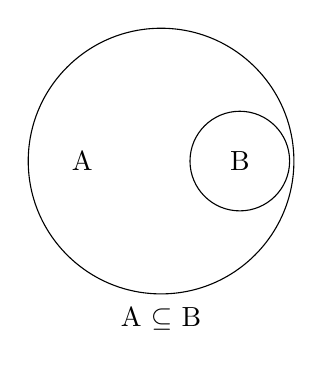
\begin{tikzpicture}
       \node at (0,0) [inner sep=1pt] (A) {A};
       \node at (2,0) (B) {B};
       \draw
          (1,0) circle [draw,radius=48pt] 
          (2,0) circle [draw,clip,radius=18pt];
       \node at (1,-2) {A $\subseteq$ B};
      \end{tikzpicture}
      \caption{Inclusion}
      \todo[inline]{Shouldn't it be B $\subseteq$ A here??}
    \end{figure}
    
    \begin{figure}
      \begin{tikzpicture}
       \node at (2,0) (B) {B};
       \filldraw [even odd rule, pattern=north east lines]
          (1,0) circle [draw,radius=48pt] 
          (2,0) circle [draw,clip,radius=18pt];
       \node at (0,0) [inner sep=1pt,fill=white] (A) {A};
       \node at (1,-2) {$\complement$\textsubscript{A}B}; 
      \end{tikzpicture}  
      \caption{Complémentaire}
    \end{figure}
                      

    L’inclusion est une \textstyleTermesapprof{relation d’ordre} (voir la \sectref{sec:3.3.30} \textit{Dépendance, dominance et transitivité} pour une définition formelle) sur les ensembles, similaire à la relation d’ordre ${\leq}$ sur les nombres (d’où la notation \textrm{${\subseteq}$}). Dire «~A \textrm{${\subseteq}$} B~» revient à dire que A est plus petit que B pour la relation d’inclusion. Néanmoins contrairement à la relation ${\leq}$, l’inclusion est un ordre \textstyleTermesapprof{partiel}, puisque deux ensembles peuvent ne pas être ordonnés l’un par rapport à l’autre, notamment lorsqu’ils sont disjoints (c’est-à-dire n’ont pas d’éléments en commun).

    À tout ensemble B inclus dans A, on peut associer le \textstyleTermesapprof{complémentaire} \textrm{${\complement}$}\textsubscript{A}B de B dans A.

    À tout ensemble E, on peut associer l’\textstyleTermesapprof{ensemble des parties} de E, noté 2\textsuperscript{E} ou \textrm{PPPFIXME}(E), avec un \textrm{PPPFIXME} comme \textit{partie}. La notation 2\textsuperscript{E} repose sur le fait que si E a \textit{n} éléments, alors 2\textsuperscript{E} a 2\textit{\textsuperscript{n}} éléments.

    Les ensembles \textrm{${\varnothing}$} et E sont respectivement le \textstyleTermesapprof{plus petit} et le \textstyleTermesapprof{plus grand élément} de 2\textsuperscript{E} pour l’inclusion.

    On ne confondra pas l’élément \textit{x} de E avec le \textstyleTermesapprof{singleton} \{~\textit{x}~\}, qui est un élément de 2\textsuperscript{E}.

    On peut définir sur 2\textsuperscript{E} deux opérations binaires, l’union et l’intersection. L’\textstyleTermesapprof{union} de A et B, notée A~\textrm{${\cup}$}~B, est l’ensemble qui contient à la fois les éléments de A et ceux de B, tandis que l’\textstyleTermesapprof{intersection} de A et B, notée A~\textrm{${\cap}$}~B, est l’ensemble des éléments communs à A et B. On peut visualiser ces ensembles sur les schémas suivants :

    \begin{figure}
      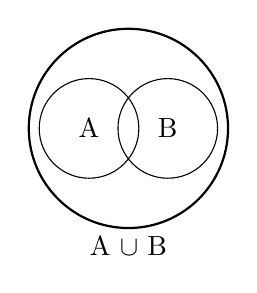
\begin{tikzpicture}
       \node at (0,0) [inner sep=1pt] (A) {A};
       \node at (1,0) (B) {B};
       \draw
          (0,0) circle [draw,radius=18pt] 
          (1,0) circle [draw,radius=18pt];
       \draw [thick]
          (0.5,0) circle [draw,radius=36pt];
       \node at (0.5,-1.5) {A $\cup$ B};
      \end{tikzpicture}
    \caption{Union}                                                                   
    \end{figure}
    
    \begin{figure}
      \begin{tikzpicture}
       \node at (0,0) [inner sep=1pt] (A) {A};
       \node at (1,0) (B) {B};
     \begin{scope}
        \clip (0,0) circle [draw,radius=18pt];
        \fill[pattern=north east lines] (1,0) circle [draw,radius=18pt];
      \end{scope}
       \draw
          (0,0) circle [draw,radius=18pt] 
          (1,0) circle [draw,radius=18pt];
       \node at (0.5,-1) {A $\cap$ B};
      \end{tikzpicture}
    \caption{Intersection}                                                                   
    \end{figure}

    L’ensemble 2\textsuperscript{E} muni des opérations binaires \textrm{${\cap}$} et \textrm{${\cup}$} et de la relation d’ordre \textrm{${\subseteq}$} possède d’excellentes propriétés similaires à celles de l’ensemble des nombres naturels muni des opérations + et \textrm{${\times}$} et de la relation ${\leq}$. En un sens, ces opérations et relations «~structurent~» l’ensemble 2\textsuperscript{E} ; une telle structure est appelée une \textstyleTermesapprof{structure algébrique}.
    }
\maths{Dualité}{%\label{sec:2.2.8}
    L’analyse distributionnelle consiste à classer les éléments en fonction de leur distribution dans des combinaisons avec d’autres éléments. La principale difficulté de l’analyse distributionnelle est que tout est interdépendant et que les éléments servent à se classifier les uns les autres. Il existe ainsi une véritable symétrie entre classes distributionnelles et familles d’environnement. Ce type de symétrie est appelé en mathématique la \textstyleTermesapprof{dualité}. Le \textstyleTermesapprof{dual} d’une classe distributionnelle est la famille des environnements compatibles avec les éléments de la classe et le \textstyleTermesapprof{dual} d’une famille d’environnements est la classe distributionnelle des éléments compatibles avec les environnements de la famille. Autrement dit, si A est une classe distributionnelle, \textbf{dual(A)} \textbf{=} \textbf{famille(A)} = “l’ensemble des environnement compatibles avec A” et, si A est une famille d’environnements, \textbf{dual(A)} \textbf{=} \textbf{classe(A)} = “l’ensemble des signes compatibles avec A”.

    Le schéma suivant illustre la dualité. La dualité lie des \textstyleTermesapprof{objets} à des \textstyleTermesapprof{propriétés~}: dans notre cas, les objets sont les signes et les propriétés les environnements (plus exactement la propriété est la compatibilité avec un environnement). Les propriétés définissent des classes d’objets, tandis que les objets définissent des familles de propriétés. Mais le procédé est totalement symétrique et on peut très bien considérer les propriétés comme nos objets et les objets comme leurs propriétés : dans ce cas, les «~propriétés~» d’une propriété donnée sont les objets compatibles avec elle.

    %%[Warning: Draw object ignored]

    Si A est une classe distributionnelle ou une famille d’environnements, dual(dual(A)) = A. La fonction «~dual~» associe donc une classe à chaque famille, laquelle est elle-même associée à cette classe. On en déduit qu’il y a exactement autant de classes distributionnelles que de familles d’environnements.

    De plus, la fonction «~dual~» possède une excellente propriété qui est de \textbf{préserver la structure algébrique} définie par les opérations \textrm{${\cap}$} et \textrm{${\cup}$} et la relation d’ordre \textrm{${\subseteq}$}, puisque dans les deux cas (que A et B soient des classes ou des environnements), on a :

    \begin{enumerate}
    \item  si A~\textrm{${\subseteq}$}~B, alors dual(B)~\textrm{${\subseteq}$}~dual(A) ; autrement dit, plus on considère d’environnements, moins il y a de signes compatibles.
    \item  dual(A~\textrm{${\cup}$}~B) = dual(A)~\textrm{${\cap}$}~dual(B) ; autrement dit, les signes compatibles avec à la fois les environnements dans A et ceux dans B sont, sans surprise, les signes qui sont à la fois compatibles avec A et compatibles avec B.
    \item dual(A~\textrm{${\cap}$}~B) = dual(A)~\textrm{${\cup}$}~dual(B).
    \end{enumerate}

    La dualité inverse les rôles de \textrm{${\cap}$} et \textrm{${\cup}$}, ce qui ne change rien à la structure, car ces deux opérations sont elles-mêmes duales l’une de l’autre. L’ensemble des classes distributionnelles et l’ensemble des familles ont donc exactement la même structure algébrique et sont le \textbf{miroir l’un} \textbf{de l’autre}.
}
\section{Signème}\label{sec:2.2.9}

Nous nous sommes intéressés jusque-là au découpage des signes linguistiques selon l’\textstyleTermes{axe syntagmatique}, c’est-à-dire selon la façon dont ils se combinent ou peuvent être décomposés. Nous allons maintenant nous intéresser à la délimitation des signes selon l’\textstyleTermes{axe paradigmatique} (voir la \sectref{sec:2.1.7} sur \textit{L’identification des unités de la langue} et l’\encadref{fig:2.2.3} sur \textit{La quatrième proportionnelle}). Nous regardons ici le paradigme des environnements pour les différentes occurrences d’une même forme afin de déterminer s’il s’agit des signifiants d’un même signe ou pas.

Considérons par exemple le segment /\textstylePhono{avãs-}/ de \textit{Le chat avançait}. On va retrouver le même segment /\textstylePhono{avãs-}/ dans des énoncés tel que \textit{Nous} \textbf{\textit{avanç}}\textit{ons grâce au vent} et \textit{L’âne ne veut plus} \textbf{\textit{avanc}}\textit{er}. On peut considérer qu’il s’agit du même signe, car sa forme est identique (l’alternance orthographique \textit{c} vs \textit{ç} n’est pas pertinente, la forme orale est identique) et que sa contribution sémantique est identique : ‘avancer’ signifie ici ‘se déplacer vers l’avant’.

Considérons maintenant d’autres occurrences de /\textstylePhono{avãs-}/ dans d’autres environnements :

\begin{figure}
%%[Warning: Draw object ignored]

\caption{Découpage de /\textstylePhono{avãs-}/ selon les axes paradigmatique et syntagmatique}
\end{figure}

Dans les énoncés \textit{Ma montre} \textbf{\textit{avanc}}\textit{e} ou \textit{Les travaux n’}\textbf{\textit{avanc}}\textit{ent pas très vite}, nous n’avons plus affaire au même signe /\textstylePhono{avãs-}/, car le sens n’est plus ‘se déplacer vers l’avant’. On peut néanmoins considérer qu’il s’agit, d’un certain point de vue, du même segment, car même si le sens est différent, il reste lié au premier sens que nous avons considéré. Il s’agit d’acceptions métaphoriques : lorsque ma montre avance, c’est comme si l’aiguille avançait plus vite que le temps ; lorsque les travaux avancent, ils se rapprochent de leur achèvement. De plus, la forme du signe est exactement la même et sa combinatoire assez similaire : \textit{avanç-} se combine toujours avec -\textit{ait} (\textit{Ma montre} \textbf{\textit{avanç}}\textit{ait}), mais par contre elle n’accepte plus de complément locatif (\textit{L’âne} \textbf{\textit{avanç}}\textit{ait vers moi ; \textsuperscript{\#}}\textit{Ma montre avance vers moi}). Bien qu’il s’agisse de trois signes différents (puisque les signifiés sont différents), nous considérons pourtant qu’ils appartiennent à une même unité, qu’on nomme généralement le verbe \textsc{avancer}.

On retrouve encore le même segment /\textstylePhono{avãs}/ dans~des énoncés tels que \textit{Pierre est en} \textbf{\textit{avance}}, \textit{Pierre a reçu une} \textbf{\textit{avance}} \textit{de 1000 euros, Pierre a fait des} \textbf{\textit{avance}}\textit{s à Marie}. Ici le sens de /\textstylePhono{avãs}/ est différent, mais surtout sa combinatoire est très différente : ce n’est plus un verbe et il ne peut plus se combiner avec un segment tel que -\textit{ait}. La forme est néanmoins identique et la parenté de sens non négligeable. Dans \textit{L’}\textbf{\textit{avance}}\textit{ment des travaux est moins rapide que prévu} ou \textit{Pierre a eu de l’}\textbf{\textit{avance}}\textit{ment}, /\textstylePhono{avãs}/ est encore un signe (\textit{avancement} est à \textit{avancer} ce que \textit{changement} est à \textit{changer}), mais sa combinatoire est encore différente puisqu’il est indissociable de \textit{{}-ment}.

Tout locuteur du français voit un lien entre toutes les occurrences d’/\textstylePhono{avãs}/ que nous avons considérées. Nous considérons donc que, d’un certain point de vue (et d’un certain point de vue seulement), il s’agit toujours du même objet : un tel objet est appelé un signème.

\begin{styleLivreImportant}
Un \textstyleTermes{signème} est un \textbf{ensemble de signes ou de quasi-signes} de \textbf{même forme} et de \textbf{sens apparentés}. (Nous considérerons des signèmes de signes de formes différentes à la \sectref{sec:2.2.20} sur l’\textit{Allomorphie}.)
\end{styleLivreImportant}

On peut repérer à l’intérieur d’un signème des sous-ensembles de signes qui ont une distribution comparable. À l’intérieur du signème /\textstylePhono{avãs}/, on repère ainsi trois (sous-)signèmes : le verbe \textsc{avancer}, le nom \textsc{avance} et le radical \textit{avance-} de \textsc{avancement}.

\loupe{Racine et signème}{%\label{sec:2.2.10}
    Jusqu’où pousser la recherche des segments communs ? Il y a dans les mots \textit{commerce} et \textit{marchand} des segments comparables (/m\textrm{ɛ}rs/ pour \textit{commerce} et /m\textrm{a}r\textrm{ʃ}/ pour \textit{marchand}) qui découlent de fait de la même \textstyleTermesapprofondissement{racine} indo-européenne /m\textrm{ɛ}rk/, que l’on retrouve non altérée dans \textit{mercantile}. Néanmoins, il est probable que les locuteurs ordinaires du français (c’est-à-dire qui ne sont pas entraînés à analyser leur langue) n’auront pas remarqué cela, malgré la forte parenté sémantique de ces mots.

    Qu’est-ce qui distingue racines et morphèmes ?

    Si nous reconnaissons dans \textit{avancement} le même signème /avãs/ que dans \textit{avançons}, c’est parce que \textit{avancement} est à \textit{avançons} ce que \textit{changement} est à \textit{changeons}. Rien de tel pour \textit{commerce} et \textit{marchand} où il n’y a aucune paire analogue. La mise en évidence d’un segment commun ne relève pas de la grammaire du locuteur et de sa connaissance \textbf{de} la langue, mais d’une connaissance \textbf{sur} la langue. Le \textbf{signème} appartient à l’étude \textstyleTermesapprofondissement{synchronique} de la langue, la \textbf{racine} à l’étude \textstyleTermesapprofondissement{diachronique} de la langue et à l’étymologie (l’étude de l’origine des mots). L’opposition entre \textstyleTermesapprofondissement{synchronie} et \textstyleTermesapprofondissement{diachronie} a été posée par Ferdinand de Saussure ; la synchronie considère un état de langue à un moment donné, tandis que la diachronie étudie les variations (du grec \textit{dia-} ‘à travers’) entre différents état de langue selon l’axe temporel (\textit{chronos}).

    Donnons deux autres exemples : \textit{avance, avant} et \textit{avantage} ont aussi une racine commune, comme le suggère les proximités de forme et de sens, mais on ne peut parler d’un même signème, puisqu’aucun des liens qui unissent ces mots n’a d’analogue en français. \textit{État} et \textit{constater} ont également une racine commune : la parenté de sens apparaît quand on pense à la synonymie entre \textit{constater} et \textit{faire état} et la parenté de forme devient évidente quand on pense qu’un autre sens de \textit{état} se dit en anglais \textit{state} (et que l’on a noté qu’il existe d’autres paires en français où un /s/ s’est effacé : \textit{été-estival, hôpital-hospitalier}).
}
\section{Signèmes minimaux : morphème et syntaxème}\label{sec:2.2.11}

Si nous considérons maintenant le signème /\textstylePhono{avãs}/, nous voyons qu’il n’est possible de décomposer aucun de ses éléments en deux signes linguistiques. On peut éventuellement essayer avec un segment /\textstylePhono{avã}/ que l’on trouve dans \textit{La plage est} \textbf{\textit{avant}} \textit{le village}, mais on ne voit pas comment la composition du sens de cet /\textstylePhono{avã}/ avec un éventuel signe /\textstylePhono{s}/ pourrait donner le signe \textit{avanç-} /\textstylePhono{avãs-}/. Proposer un signe \textstylePhono{/s/} n’aurait de sens qu’au cas où pour un autre signe X au moins, l’ajout d’un \textstylePhono{/s/} créait le sens ‘se déplacer dans la direction X’, c’est à dire si /\textstylePhono{avã}/ et /s/ se combinaient proprement. Le signème /\textstylePhono{avãs}/ est donc indécomposable.

\begin{styleLivreImportant}
Un \textstyleTermes{morphème} est un signème dont aucun signe n’est décomposable proprement.
\end{styleLivreImportant}

Les morphèmes sont donc les signèmes minimaux du point de vue de l’opération de combinaison propre ${\boxplus}$. Nous pouvons considérer de même les signèmes minimaux du point de vue de la combinaison libre ${\oplus}$, que nous appelons les syntaxèmes.

\begin{styleLivreImportant}
Un \textstyleTermes{syntaxème} est un signème de signes de la même classe distributionnelle dont certains se combinent librement et dont aucun n’est une combinaison libre de signes.
\end{styleLivreImportant}

Les morphèmes sont les \textbf{unités minimales de la morphologie} et les syntaxèmes sont les \textbf{unités minimales de la syntaxe}. La définition des syntaxèmes sera précisée dans le \chapref{sec:3.1}.

Reprenons l’exemple du signème /\textstylePhono{avãs}/ : il s’agit d’un morphème, puisqu’aucun de ses éléments n’est décomposable proprement. Il contient deux syntaxèmes que sont \textsc{avancer} et \textsc{avance}. Enfin, \textsc{avancement} est un syntaxème, puisqu’aucune de ses acceptions n’est décomposable librement (seul un petit nombre de morphèmes verbaux permettent la combinaison avec \textit{{}-ment}). Il est néanmoins décomposable proprement et contient une occurrence du morphème /\textstylePhono{avãs}/.

\loupe{Les termes \textit{morphème} et autres \textit{X-èmes}}{%\label{sec:2.2.12}
    La première étude des règles morphologiques d’une langue remonte à 2500 ans au moins. Il s’agit de l’extraordinaire description du sanskrit védique faite par le linguiste indien Pā\textrm{ṇ}ini, qui comprend une description des morphèmes du sanskrit et des règles de combinaison de leurs signifiants. Les termes \textit{morphème} et \textit{phonème} sont introduits dans les années 1880 par le linguiste polonais Baudouin de Courtenay. La définition formelle des morphèmes et le principe de commutation doivent beaucoup aux travaux des distributionnalistes américains sur les langues amérindiennes (voir l’\encadref{fig:2.1.8} sur \textit{Structuralisme et distributionnalisme}).

    Les termes en -\textit{ème} vont foisonner au cours du 20\textsuperscript{e} siècle. Les termes \textit{lexème} et \textit{grammème} sont couramment utilisés pour désigner respectivement les unités du lexique et celles de la grammaire. Nous introduisons \textit{syntaxème} pour désigner les unités minimales de la syntaxe, qu’elles soient lexicales comme le \textit{lexème} ou grammaticales comme le \textit{grammème}. Le terme \textit{syntaxème} (ou la variante \textit{syntactème}) a été utilisé marginalement par quelques auteurs, mais ne s’est jamais imposé, d’autant que c’est le mot qui est généralement considéré comme l’unité minimale de la syntaxe (contrairement au point de vue défendu ici qui considère qu’il s’agit du syntaxème). Le terme \textit{sémantème}, que nous utiliserons pour désigner les unités minimales de la sémantique, est beaucoup plus courant et a été utilisé par Charles Bally ou Igor Mel’čuk pour désigner les sens lexicaux. Nous lui donnons un sens un peu différent en l’utilisant pour désigner des signes (et pas seulement des signifiés) (voir \chapref{sec:2.3} sur \textit{Sémantèmes et syntaxèmes}). Tous les termes que nous venons de mentionner (\textit{morphème, lexème, grammème, syntaxème, sémantème}) désignent, dans l’acception dans laquelle nous les utilisons, des ensembles de signes. Pour finir, nous introduisons le terme \textit{signème} pour désigner tout ensemble de signes d’un de ces types.
}
\section{Lexème, flexion et grammème}\label{sec:2.2.13}

On distingue deux principaux types de syntaxèmes : les syntaxèmes lexicaux ou lexèmes et les syntaxèmes flexionnels ou grammèmes.

\begin{itemize}
\item \textsc{avancer} est un \textstyleTermes{syntaxème lexical} ou \textstyleTermes{lexème~}: il appartient à une classe distributionnelle \textstyleTermes{ouverte} de syntaxèmes, c’est-à-dire qu’il peut commuter avec un très grand nombre de syntaxèmes, potentiellement illimité (cet ensemble est celui des verbes). De plus, ses sens sont assez précis pour être paraphrasés. Par exemple, dans l’énoncé \textit{Le chat avançait}, \textsc{avancer} signifie ‘se déplacer vers l’avant’ et il commute avec sa définition : \textit{Le chat se déplaçait vers l’avant} est une paraphrase de \textit{Le chat avançait}.
\item {}-\textit{ait} est une \textstyleTermes{flexion}. Il s’agit d’une combinaison de plusieurs syntaxèmes, qui comprend notamment la combinaison libre d’un temps (l’imparfait) et d’un accord en nombre et personne. Les syntaxèmes qui composent une flexion s’appellent des \textstyleTermes{syntaxèmes flexionnels} ou \textstyleTermes{grammèmes}. Flexions et syntaxèmes flexionnels appartiennent à des classes distributionnelles \textstyleTermes{fermées} d’éléments, c’est-à-dire qu’ils commutent avec un nombre restreint d’éléments similaires dont on peut faire la liste exhaustive (il y a par exemple 51 flexions possibles pour un verbe du français : 6 formes pour chacun des 7 «~temps~» simples, 4 formes pour chacun des deux participes, auxquelles il faut encore ajouter la forme infinitive ; 51 = 7${\times}$6 + 2${\times}$4 + 1). Les grammèmes expriment des significations grammaticales qui ne peuvent être paraphrasées facilement.
\end{itemize}

Lexème verbal et flexion ne peuvent donc pas être utilisés de manière \textstyleTermes{autonome}. Le lexème et sa flexion sont \textstyleTermes{indissociables} l’un de l’autre : une flexion verbale ne s’utilise pas sans une base verbale et un lexème verbal ne s’utilise pas sans flexion. Ceci nous amène à la définition du mot, sur laquelle nous reviendrons au \chapref{sec:4.1} : un \textstyleTermes{mot} est grosso modo un signe linguistique autonomisable minimal, c’est-dire dont les parties sont indissociables et donc non-autonomisables.

Du fait que les lexèmes verbaux ne sont pas autonomisables, il est d’usage de les nommer par l’une de leurs formes fléchies. L’usage en français est d’utiliser la forme infinitive. Cet usage est purement conventionnel (et pédagogiquement assez mauvais puisque le radical de l’infinitif n’est généralement pas le radical de base ; voir l’\encadref{fig:2.2.23} sur \textit{Syntaxème zéro et troncation en français}) ; par exemple en grammaire latine, il est d’usage de nommer un lexème verbal par la forme de la 1\textsuperscript{ère} personne du singulier du présent (lat. \textsc{amo} ‘j’aime’) et en grammaire arabe par la forme de la 3\textsuperscript{ème} personne du singulier du passé (ar. \textsc{kataba} ‘il a écrit’). Pour éviter toute confusion entre le lexème et la forme infinitive, nous notons le premier en petites majuscules, \textsc{avancer}, et la deuxième en italique, \textit{avancer}. Les syntaxèmes flexionnels sont désignés par des termes métalinguistiques : présent, pluriel, etc. La forme \textit{avancer} est la combinaison de \textsc{avancer} et de l’infinitif :

\ea
\textit{avancer} = \textsc{avancer} ${\oplus}$ infinitif.
\z

\section{Signème libérable, radical, affixe}\label{sec:2.2.14}

Nous allons caractériser les occurrences des morphèmes au sein des lexèmes, c’est-à-dire les \textstyleTermes{morphèmes sous-lexicaux}. Un lexème qui peut être décomposé en plusieurs morphèmes est dit \textstyleTermes{complexe}.

\begin{styleLivreImportant}
Un signème est dit \textstyleTermes{libérable} s’il existe des environnements dans lesquels ce signème commute librement. Un \textstyleTermes{morphème libérable} est donc un morphème qui contient un syntaxème. Lorsque ce syntaxème est lexical, le morphème est dit \textstyleTermes{lexical}.
\end{styleLivreImportant}

Cette propriété est utilisée pour classifier les morphèmes constitutifs d’un lexème complexe. Si l’on considère le syntaxème \textit{brûlure}, qui se décompose en \textit{brûl}${\boxplus}$\textit{ure}, on constate que \textit{brûl-} est libérable, puisqu’il commute librement dans \textit{nous brûlons}, mais \textit{{}-ure} n’est pas libérable, puisqu’il n’existe aucun environnement où -\textit{ure} commute librement.

\begin{styleLivreImportant}
Un morphème, lorsqu’il est l’unique morphème lexical d’un lexème, est appelé le \textstyleTermes{radical} du lexème. Un morphème non lexical est appelé un \textstyleTermes{affixe}. Lorsqu’il précède le radical, il s’agit d’un \textstyleTermes{préfixe} et lorsqu’il le suit d’un \textstyleTermes{suffixe}.
\end{styleLivreImportant}

Il existe également des lexèmes construits uniquement avec des morphèmes non libérables. En français, un certain nombre de lexèmes, appelés composés savants, sont construits avec deux morphèmes lexicaux empruntés au grec ancien (dont certains sont devenus libérables) : \textit{sismo}${\boxplus}$\textit{graphe, sismo}${\boxplus}$\textit{logue, grapho}${\boxplus}$\textit{logue, géo}${\boxplus}$\textit{graphe, géo}${\boxplus}$\textit{thermie, thermo}${\boxplus}$\textit{mètre, métro}${\boxplus}$\textit{nome}, etc. De tels morphèmes, dont le statut est intermédiaire entre affixe et radical, sont appelés des \textstyleTermes{confixes}, car ils doivent être associés par paire pour former un lexème.

Il faut noter que les termes de \textit{libre} et de \textit{libérable} sont définis par des critères purement distributionnels et recouvrent donc des notions syntaxiques. Ils ne doivent pas être confondus avec un autre emploi du terme \textit{libre} dû à Bloomfield qui est proche de ce que nous avons appelé l’autonomisabilité et qui conduit à appeler \textit{forme liée} tout affixe. Dans notre terminologie, au contraire, les \textbf{syntaxèmes flexionnels}, bien qu’étant des affixes, se combinent librement par définition et sont parfaitement \textbf{libérables}. Par contre, ils ne sont \textbf{pas autonomisables}, puisqu’ils sont indissociables de lexèmes.

Les notions de radical et d’affixe doivent être étendues par analogie. Ainsi, un quasi-morphème comme \textit{struct-}, bien que non libérable, est également considéré comme un élément lexical et comme le radical de \textit{structure} et de \textit{construction}, car il commute avec des morphèmes lexicaux.

A l’inverse, certains préfixes du français présentent un cas limite d’affixe, puisqu’ils appartiennent à des morphèmes prépositionnels comme le \textit{en} de \textit{il} \textbf{\textit{en}}\textit{terre} ou le \textit{sur} de \textit{il} \textbf{\textit{sur}}\textit{estime}. On considère quand même qu’il s’agit d’affixes, car les prépositions simples forment une classe fermée et sont donc moins lexicales que les morphèmes qui ont des emplois en tant que syntaxèmes appartenant à des classes ouvertes. De plus, la classe distributionnelle des préfixes du français contient quand même une bonne proportion de morphèmes non libérables, comme \textit{con-} ou \textit{in-}, et qui commutent avec les autres (\textbf{\textit{com}}\textit{prendre} vs \textbf{\textit{sur}}\textit{prendre}, \textbf{\textit{in}}\textit{estimable} vs \textbf{\textit{sur}}\textit{estimer}).

\section{Dérivation et composition}\label{sec:2.2.15}

La plupart des lexèmes complexes du français sont construits avec un radical et un certain nombre d’affixes. Par exemple, le lexème \textit{détournement} est construit avec le radical \textit{tourn-}, le préfixe \textit{dé-} et le suffixe \textit{{}-ment}. Les lexèmes complexes comportant un unique morphème lexical sont appelés des \textstyleTermes{dérivés morphologiques}. L’opération qui consiste à ajouter un affixe à un lexème pour former un nouveau lexème est appelée la \textstyleTermes{dérivation morphologique}.

Il existe aussi des lexèmes construits avec plusieurs morphèmes lexicaux, comme \textit{soutien-gorge} ou \textit{bonhomme} : de tels syntaxèmes sont appelés des \textstyleTermes{composés morphologiques}. L’opération qui consiste à combiner deux lexèmes pour former un nouveau syntaxème est appelée la \textstyleTermes{composition morphologique}. Un composé peut être la source d’une dérivation comme dans \textit{bonhommie}.

On peut associer à un lexème complexe une structure morphologique en regardant les portions du lexème qui sont libérables. Une \textstyleTermes{unité morphologique} est soit un morphème, soit une portion libérable d’un lexème. Les unités morphologiques de \textit{détournement} sont les morphèmes \textit{dé-, tourn-} et -\textit{ment} et les combinaisons \textit{détourn-} (\textit{il} \textbf{\textit{détourn}}\textit{ait}) et \textit{détournement.} Par contre °\textit{tournement} n’est pas libérable. On en déduit une \textstyleTermes{structure morphologique} que nous pouvons représenter dans ce cas par un parenthésage : \textit{détournement} = (\textit{dé}${\boxplus}$\textit{tourn})${\boxplus}$\textit{ment}. Ceci induit un \textstyleTermes{chemin dérivationnel} menant du radical du lexème au lexème complet par combinaisons successives de morphèmes. Pour \textit{détournement}, le chemin est \textit{tourn}(\textit{er}) → \textit{détourn}(\textit{er}) → \textit{détournement} et pas \textit{tourn}(\textit{er}) → °\textit{tournement} → \textit{détournement}. Cela signifie que, dans la façon dont est perçu le lexème \textit{détournement}, c’est \textit{dé}{}- qui s’affixe d’abord à \textit{tourn}{}-, puis -\textit{ment} au tout.

L’étude des \textstyleTermes{morphèmes sous-lexicaux}, c’est-à-dire des occurrences d’un morphème à l’intérieur d’un lexème, ne relève pas de la syntaxe et est donc hors de la visée de cet ouvrage. Une telle étude concerne la construction des lexèmes, c’est-à-dire la \textstyleTermes{morphologie constructionnelle} et la \textstyleTermes{lexicologie}. Cette notion est néanmoins essentielle à la compréhension de ce que sont les syntaxèmes et de ce qui les différencie des occurrences liées des morphèmes.

\loupe{«~Syntaxe~» des morphèmes sous-lexicaux}{%\label{sec:2.2.17}
    Lorsqu’on parle de syntaxe, on parle normalement de combinatoire libre (voir la \sectref{sec:3.1.6} sur \textit{Syntaxe et morphologie}) et lorsqu’on parle de combinatoire libre, on parle de combinaisons qui sont faites par le locuteur au moment de la production d’un nouvel énoncé (voir l’\encadref{fig:2.2.6} sur \textit{Liberté de combinaison et opposition parole/langue}). La combinatoire des sous-morphèmes relève au contraire de la structure d’unités déjà construites et stockées dans le lexique mental du locuteur (même s’il existe la possibilité de construire de nouvelles unités lors de la production avec les constructions productives). Il en découle que l’histoire constructionnelle de ces unités se fait sur un temps beaucoup plus long, bien qu’il en reste des traces en synchronie (par la commutation propre avec d’autres morphèmes). On peut alors se poser la question suivante : la structure des combinaisons de sous-morphèmes est-elle ou non de la même nature que celle des syntaxèmes ?

    Nous étudierons en détail la structure des combinaisons syntaxiques dans la partie 3, dont c’est le sujet central. Les outils que nous introduirons peuvent aussi s’appliquer à la description des combinaisons morphologiques. Nous opposerons en particulier deux approches principales de la structure syntaxique, la structure de dépendance et la structure de constituants. La principale différence entre les deux approches reposent sur ce qu’elles encodent prioritairement (voir l’\encadref{fig:3.4.16} \textit{Dépendance et constituance se complètent}). Les structures de constituants permettent d’encoder naturellement l’ordre dans lequel les combinaisons ont lieu et c’est ce que nous avons utilisé pour présenter l’analyse de \textit{détournement}, car nous voulions indiquer que lors de l’histoire dérivationnelle de ce mot, \textit{tourn-} s’est d’abord combiné avec \textit{dé-}, puis \textit{{}-ment}. Ils existent des cas où l’histoire dérivationnelle n’est pas aussi claire en synchronie. Tel est le cas par exemple de \textit{châtaigneraie, pommeraie} ou \textit{orangeraie}. Il s’agit a priori du suffixe \textit{{}-aie} qui appliqué à un nom d’arbre désigne un groupe d’arbre, comme dans \textit{chênaie} ‘groupe de chênes’ ou \textit{peupleraie} ‘groupe de peupliers’, avec en plus une alternance -\textit{ier} /je/ → -\textit{er} /ʁ/. On aurait donc \textit{châtaigneraie} = (\textit{châtaigne}\textrm{${\boxplus}$}\textit{ier})\textrm{${\boxplus}$}\textit{aie}. Mais on peut aussi analyser ces dérivations comme le résultat direct de l’application du suffixe \textit{{}-eraie}, lequel suffixe se rencontre dans \textit{chêneraie} ‘groupe de chênes’ (lexème considéré comme fautif mais largement attesté). On peut représenter cette ambiguïté en utilisant une représentation non parenthésée de la dérivation (\textit{châtaigneraie} = \textit{châtaigne}\textrm{${\boxplus}$}\textit{ier}\textrm{${\boxplus}$}\textit{aie}), qui s’apparente alors à une structure de dépendance, puisqu’on n’indique que \textit{{}-ier} se combine aussi bien avec \textit{châtaigne} que \textit{{}-aie} sans spécifier quelle combinaison a lieu en premier.
}
\loupe{Sémantique des morphèmes sous-lexicaux}{%\label{sec:2.2.18}
    Le fait qu’un affixe soit toujours un morphème non libérable influe sur la nature même de son sens : l’affixe ne peut jamais être «~isolé~» et son sens ne peut pas être saisi de manière autonome. Le sens d’un affixe n’apparaît que dans la \textbf{relation entre deux lexèmes} : le sens de -\textit{ure} naît de la relation entre \textsc{blessure} et \textsc{blesser}. Ainsi le sens d’un tel morphème est nécessairement de nature \textbf{opératoire} : il n’est exprimable que dans la relation entre deux sens. Le sens de -\textit{ure} est le sens de l’opération qui permet de construire ‘blessure’ à partir de ‘blesser’ et d’autres paires du même type : une X-ure est le résultat obtenu en X-ant.

    Il existe aussi des morphèmes, comme le -\textit{aume} de \textit{royaume,} qui n’apparaissent que dans un seul lexème dont la diagrammaticité est suffisamment claire pour qu’on attribue un sens au morphème : le fait que le lien sémantique entre \textit{royaume} et \textit{roi} soit assez simple (un royaume est le territoire sous la tutelle d’un roi) et que la paire \textit{roi}{}-\textit{royaume} soit parallèle à d’autres paires comme \textit{prince}{}-\textit{principauté} ou \textit{duc}{}-\textit{duché}, permet de définir facilement le sens (opératoire) de -\textit{aume}. Par contre, \textit{fur}, qui est pourtant un mot, mais qui n’apparaît que dans \textit{au fur et à mesure} n’a plus de sens accessible en français contemporain, car la construction dans laquelle il entre est isolée et qu’il n’y a jamais de commutation possible sur \textit{fur}. De même, beaucoup de locuteurs du français vont utiliser une locution comme \textit{être dans le collimateur} sans avoir aucune idée de ce qu’est un collimateur (voir la \sectref{sec:3.1.3} sur \textit{Le collimateur et la sellette} pour d’autres exemples).
}
\eiffel{À la limite entre morphème sous-lexical et syntaxème flexionnel}{%\label{sec:2.2.19}
    La notion de commutation libre est \textstyleTermesapprofondissement{graduelle} et il est parfois difficile pour certains morphèmes de les situer entre morphème sous-lexical et syntaxème (flexionnel). Le cas du morphème -\textit{ment} qui transforme un adjectif en adverbe est un cas intéressant de morphème qui ne commute pas librement, mais s’en approche néanmoins. Dans de nombreux cas, le changement de partie du discours opéré par \textit{{}-ment} ne s’accompagne d’aucun changement de sens, ce qui signifie que la commutation est propre : cf. le passage de \textit{un départ rapide} à \textit{partir rapidement} ou de \textit{une réflexion intense} à \textit{réfléchir intensément}. Mais la dérivation en -\textit{ment} n’est pas systématiquement possible : cf. \textit{une réflexion poussée}/\textit{élaborée} vs *\textit{réfléchir poussément}/\textit{élaborément}, \textit{un départ inattendu} vs *\textit{partir inattendument}. Même des adjectifs très courant comme \textsc{gros} n’ont pas d’adverbe correspondant : \textit{faire une grosse erreur} vs *\textit{se tromper grossement}. Certains adverbes en -\textit{ment} sont fort peu diagrammatiques et ne peuvent pas être décomposés proprement, comme \textit{vraiment}, \textit{carrément} ou \textit{vertement}. En conséquence, la classe des éléments qui se combine avec \textit{{}-ment} comporte pas mal d’irrégularités et est par exemple différente de la classe des adjectifs qui se combinent avec \textit{de façon}, puisqu’on a \textit{de façon poussée, élaborée} ou \textit{inattendue} et pas \textit{de façon verte}. On peut également noter quelques irrégularités morphologiques (voir la \sectref{sec:2.2.20} sur l’\textit{Allomorphie}) dans la combinaison de \textit{{}-ment} et d’un adjectif, toutefois la combinaison libre des verbes avec leur flexion comprend davantage encore d’idiosyncrasies, donc les arguments purement morphologiques ne permettent pas de décider s’il s’agit de combinaison libre ou non.

    Un autre cas discutable est le «~genre~» des noms. Le genre des noms ne doit pas être confondu avec le genre des adjectifs. Le genre des adjectifs est un syntaxème flexionnel qui se combine librement avec l’adjectif. Il n’a aucune contribution sémantique et sert seulement à mieux marquer la dépendance entre le nom et l’adjectif qui le qualifie (ce rôle syntaxique constitue la signification du syntaxème flexionnel). Certains noms varient apparemment en genre comme \textit{lion} vs \textit{lionne}, \textit{acteur} vs \textit{actrice} ou \textit{prince} vs \textit{princesse}. Mais dans ce cas, l’opposition est sémantique et marque une opposition de sexe : la lionne est la femelle du lion. Elle peut s’accompagner d’une variation de sens plus importante, puisque par exemple un prince est toujours le fils d’un roi, tandis qu’une princesse peut être la fille d’un roi ou la femme d’un prince. De même, un lion et une lionne possèdent des différences morphologiques suffisamment importantes, comme la crinière, pour qu’il soit bizarre de dire qu’une lionne est un lion femelle. De plus, cette alternance de genre est assez capricieuse avec de nombreux noms dons le genre est fixe (\textit{grenouille, girafe, chacal, moustique,} etc.), même si l’alternance de sexe reste signifiante et plusieurs cas où deux formes sans liens morphologiques existent (\textit{poule} et \textit{coq} ou \textit{jument} et \textit{étalon}). Citons encore les nombreux trous que des néologismes comme \textit{auteure} ou \textit{professeure} peinent encore à combler. Il y a donc toutes les raisons de considérer le /\textstylePhonoApprofondissement{ɛs}/ de /\textstylePhonoApprofondissement{prɛsɛs}/ \textit{princesse} comme un morphème sous-lexical plutôt qu’un syntaxème flexionnel.
}
\section{Allomorphie}\label{sec:2.2.20}

Nous n’avons jusque-là considéré que des signèmes dont tous les éléments ont le même signifiant. Il y a néanmoins de bonnes raisons d’élargir la notion de signème et d’accepter des alternances de formes. Ainsi là où le verbe \textsc{avancer} présente une seule forme /\textstylePhono{avãs-}/, le verbe \textsc{aller} présentent quatre formes : /\textstylePhono{v/-} dans \textit{tu} \textbf{\textit{v}}\textit{as}, /\textstylePhono{al/-} dans \textit{nous} \textbf{\textit{all}}\textit{ons}, /\textstylePhono{i/-} dans \textit{nous} \textbf{\textit{i}}\textit{rons}, /\textstylePhono{aj/-} dans \textit{qu’il} \textbf{\textit{aill}}\textit{e}. On veut pourtant regrouper ces formes parce que \textbf{\textit{all}}\textit{+ons} est à \textit{avanç+ons} ce que \textbf{\textit{i}}\textit{+rons} est à \textit{avance+rons}. Nous dirons que \textit{all-} et \textit{i-} sont des allomorphes.

\begin{styleLivreImportant}
Pour que les signes A\textsubscript{1} et A\textsubscript{2} soient des \textstyleTermes{allomorphes}, il faut que A\textsubscript{1} et A\textsubscript{2} aient des signifiants différents, mais qu’il existe un signe A’ et un certain nombre de signes B et B’ tels que A\textsubscript{1}+B soit à A\textsubscript{2}+B’ ce que A’+B est à A’+B’.
\end{styleLivreImportant}

Cette propriété est bien vérifiée par notre premier exemple : A\textsubscript{1} = \textit{al-}, A\textsubscript{2} = \textit{i-}, A’ = \textit{avanç-}, B = \textit{{}-ons}, B’ = -\textit{rons} et A\textsubscript{1}+B = \textit{allons} est à A\textsubscript{2}+B’ = \textit{irons} ce que A’+B = \textit{avançons} est à A’+B’ = \textit{avancerons}. Deux allomorphes sont donc des signes différents, puisqu’ils ont des signifiants différents, mais ils se comportent ensemble comme s’ils formaient un unique signe, puisqu’ils commutent avec un même signe A’. On traduit cela en demandant qu’ils commutent proprement avec un tel signe dans un certain nombre d’environnements.

La notion d’allomorphie nous permet d’étendre la notion de morphème.

\begin{styleLivreImportant}
Un \textstyleTermes{morphème polymorphique} est la réunion de plusieurs «~morphèmes~» de formes différentes qui sont des allomorphes les uns des autres. Un \textstyleTermes{morphe} est un sous-ensemble de signes d’un morphème qui possèdent le même signifiant.
\end{styleLivreImportant}

La première propriété que nous avons donnée pour définir l’allomorphie n’est pas suffisante. Une autre propriété nécessaire pour être des allomorphes est de se ressembler. Il y a en fait deux types de ressemblance possibles et ainsi deux notions d’allomorphie : l’une, syntaxique, est une allomorphie au sein d’un syntaxème, basée sur une similarité de syntactique ; l’autre, morphologique, est une allomorphie au sein d’un morphème, basée sur la similarité des formes.

\begin{styleLivreImportant}
Les signes A\textsubscript{1} et A\textsubscript{2} sont des \textstyleTermes{allomorphes (syntaxiques)}\textbf{ }si A\textsubscript{1} et A\textsubscript{2} ont des formes différentes, mais des sens identiques et s’il existe un syntaxème A’ dont l’ensemble des contextes possibles réunit les contextes possibles de A\textsubscript{1} et A\textsubscript{2}.
\end{styleLivreImportant}

Le cas de \textsc{aller} vu précédemment illustre l’allomorphie syntaxique. La réunion des paradigmes de flexion des différents allomorphes de \textsc{aller} comprend 51 formes et est équivalent au paradigme de flexion de n’importe quel verbe.

Un autre exemple d’allomorphie syntaxique est l’alternance des formes /ɛ/ vs /j/ pour l’imparfait. En effet, ces deux formes ont exactement les mêmes sens et elles possèdent, à elles deux, la même extension que le syntaxème zéro du présent ou le syntaxème /ʁ/ du futur.

Le deuxième cas d’allormorphie nous concerne moins, car il ne relève pas de la syntaxe.

\begin{styleLivreImportant}
Les signes A\textsubscript{1} et A\textsubscript{2} sont des \textstyleTermes{allomorphes (morphologiques)} si A\textsubscript{1} et A\textsubscript{2} ont des formes différentes mais similaires, des sens apparentés et s’il existe des signes A’, B et B’ tels que A\textsubscript{1}+B soit à A\textsubscript{2}+B’ ce que A’+B est à A’+B’.
\end{styleLivreImportant}

Dans le cas de l’allomorphie morphologique, il n’y a plus identité de sens et la combinatoire est généralement très différente : il faut donc que A\textsubscript{1} et A\textsubscript{2} possèdent une proximité formelle suffisante pour qu’on considère qu’ils sont parents. Par exemple, \textit{écriv}{}- et \textit{écrit}{}- sont des allomorphes, car \textit{écrit+ure} est à \textit{écriv+ons} ce que \textit{sculpt+ure} est à \textit{sculpt+ons} et /ekʁit/ et /ekʁiv/ sont formellement proche. La différence de forme peut être plus importante si elle se retrouve plusieurs fois : \textit{construct}{}- et \textit{construis}{}- sont des allomorphes, car \textit{construction} est à \textit{construisons} ce que \textit{instruction} est à \textit{instruisons} ou ce que \textit{destruction} est à \textit{détruisons}.

Par contre, même si \textit{coup} est à \textit{frapp+ons} ce que \textit{gifle} est à \textit{gifl+ons}, on ne dira pas que \textit{coup} est un allomorphe de \textit{frapp-}. Il y a là une trop grande distance formelle. On dira plutôt que \textit{coup} est un \textstyleTermes{supplétif} de \textit{frapp-}.

En général, les allomorphes d’un signème sont en \textstyleTermes{distribution complémentaire}, c’est-à-dire que leurs environnements respectifs sont incompatibles (voir la notion de \textit{complémentaire} en \textit{Théorie des ensembles} dans la \sectref{sec:2.2.7}). Mais il existe aussi des cas d’alternance de forme dans un même environnement. Par exemple le verbe \textsc{balayer} possèdent deux allomorphes /\textstylePhono{balɛ}/ et /\textstylePhono{balɛj}/ qui peuvent alterner avec certaines flexions : \textit{ils balaient} vs \textit{ils balayent}.

\eiffel{Alternance vocalique en français : allomorphie ou alternance phonologique ? }{%\label{sec:2.2.21}
    Identifier le nombre d’allomorphes d’un morphème ne va pas nécessairement de soi. Ainsi le verbe \textsc{céder} alterne apparemment deux formes : \textit{céd}{}- [\textstylePhonoApprofondissement{sed}] dans \textit{nous cédons} et \textit{cèd}{}- [\textstylePhonoApprofondissement{sɛd}] dans \textit{il cède}. Si [e] et [\textstylePhonoApprofondissement{ɛ}] peuvent être distinctifs dans les syllabes ouvertes (CV) finales (cf. l’opposition entre \textit{été} /\textstylePhono{ete}/ vs \textit{était} /\textstylePhono{etɛ}/ en français parisien), ils se neutralisent dans les autres positions et forment ce qu’on appelle un archiphonème, que nous noterons /\textstylePhonoApprofondissement{E}/ : en syllabe fermée, /\textstylePhonoApprofondissement{E}/ est prononcé [\textstylePhonoApprofondissement{ɛ}] et, en syllabe ouverte non finale, il est prononcé /\textstylePhonoApprofondissement{e}/. Ainsi l’alternance relève complètement de la phonologie du français et \textsc{céder} possède donc un unique morphe /\textstylePhonoApprofondissement{cEd}/. La situation est différente pour \textsc{appeler} qui présente une \textstyleTermes{alternance} entre \textit{appell}{}- /\textstylePhonoApprofondissement{apɛl}/ dans \textit{il appelle} et \textit{appel}{}- /\textstylePhonoApprofondissement{apəl}/ dans \textit{nous appelons~}: ici l’alternance n’a plus de motivation phonologique en français contemporain et il y a bien allomorphie. Le fait que la distribution des deux allomorphes de \textsc{appeler} soit identique à celle des deux prononciations de \textsc{céder} laisse supposer que cette allomorphie résulte d’une alternance phonologique aujourd’hui morte, du même type que celle bien vivante de \textsc{céder}. Une allomorphie de même distribution (et de même origine) se trouve avec les verbes \textsc{mourrir} ou \textsc{pouvoir} (\textit{il} \textbf{\textit{meur}}\textit{t} vs \textit{nous} \textbf{\textit{mour}}\textit{ons}, \textit{il} \textbf{\textit{peu}}\textit{t} vs \textit{nous} \textbf{\textit{pouv}}\textit{ons}). Nous verrons un autre cas distributionnellemnt similaire à l’allomorphie avec les verbes dit du 2\textsuperscript{ème} groupe (dans l’\encadref{fig:2.2.25} sur \textit{Syntaxème zéro et troncation en français}).
}
\section{Amalgame, alternance et mégamorphe}\label{sec:2.2.22}

Nous avons fait jusque-là comme si les signifiants se combinaient de manière \textstyleTermes{concaténative}, c’est-à-dire en s’enchaînant les uns à la suite des autres. Il existe certaines situations où il est difficile de trouver la limite entre un lexème et sa flexion. Par exemple, la forme verbale [\textit{nous}] \textit{sommes} entre dans le paradigme des formes du verbe \textsc{être} et se décompose normalement en un morphe du morphème \textsc{être} et une flexion. Les formes en \textit{{}-mes} de la 1\textsuperscript{ère} personne du pluriel ne se rencontrent plus qu’au passé simple (\textit{nous chant}+\textit{â}+\textit{mes}) et de surcroît aucune autre forme de \textsc{être} n’a le radical \textit{som-}. Il s’agit donc, pour \textit{sommes}, d’une forme amalgamée exprimant conjointement le lexème \textsc{être} et sa flexion.

\begin{styleLivreImportant}
Une combinaison de syntaxèmes dont le signifiant est \textstyleTermes{indécomposable} est appelée un \textstyleTermes{amalgame} ou \textstyleTermes{mégamorphe fort}. Les syntaxèmes au sein d’un amalgame sont réalisés de manière \textstyleTermes{cumulative}.
\end{styleLivreImportant}

Même des syntaxèmes normalement réalisés par des mots séparés peuvent s’amalgamer, comme \textit{au} /\textstylePhono{o}/ en distribution complémentaire avec \textit{à la} /\textstylePhono{ala}/. Les flexions, c’est-à-dire les combinaisons de syntaxèmes flexionnels, sont souvent des mégamorphes forts : par exemple, si on considère que l’accord verbal -\textit{ons} /\textstylePhono{ɔ}/ combine un accord en personne (1\textsuperscript{ère} personne) et un accord en nombre (pluriel) (voir discussion sur ce point dans la \sectref{sec:4.2.13} sur les \textit{Catégories flexionnelles abstraites}), cette combinaison est un mégamorphe fort.

Un signe tel que \textit{chevaux} \textstylePhono{/ʃəvo/ pose un problème un peu différent. Ici le principe de commutation s’applique à l’ensemble du signe, signifiant compris : \textit{chevaux} est à \textit{cheval} ce que \textit{animaux} est à \textit{animal}. Il n’est néanmoins pas satisfaisant de décomposer \textit{chevaux} en \textit{chev}+\textit{aux}, car les dérivés de \textit{cheval/chevaux} prennent \textit{cheval} comme base : chevalin, chevalier} ou \textit{chevaleresque}. Même chose pour les dérivés d’autres lexèmes en -\textit{al/-aux~}: \textbf{\textit{animal}}\textit{ité,} \textbf{\textit{métall}}\textit{ique}, \textbf{\textit{canal}}\textit{iser}, etc. Il faut donc considérer que le radical du lexème \textsc{cheval} est \textit{cheval} et que le pluriel est réalisé par une \textstyleTermes{alternance} \textstylePhono{/al/} ${\Rightarrow}$ \textstylePhono{/o/}. Le signifiant de cet allomorphe du pluriel est ainsi traité comme une opération qui transforme le segment terminal du radical /al/ en /o/. En conséquence, le signifiant du pluriel ne peut donc pas être séparé du signifiant lexical dans la forme \textstylePhono{/ʃəvo}/ et cette forme est ainsi \textstyleTermes{non segmentable}, bien qu’elle soit obtenue par la \textbf{combinaison régulière} du signifiant lexical et d’une apophonie.

\begin{styleLivreImportant}
Un signe dont le signifiant est décomposable sans être segmentable est appelé un \textstyleTermes{mégamorphe faible}.
\end{styleLivreImportant}


\loupe{Flexions irrégulières}{%\label{sec:2.2.23}
    Pourquoi les formes verbales du présent sont plus irrégulières que celle des autres temps ? Pourquoi les participes passés sont plus irréguliers que les participes présents ? Pourquoi les formes des verbes très utilisées comme \textsc{être,} \textsc{avoir} ou \textsc{aller} sont plus irrégulières que les autres ? Parce que les formes les moins courantes sont construites par analogie par les locuteurs et sont donc régulières, alors que les formes très courantes sont apprises dans leur globalité. Dans ces formes qui ne sont plus décomposées (ou plutôt qui ne sont pas composées au moment de leur utilisation), les signifiés des syntaxèmes tendent à se fusionner. Ceci est vrai dans toutes langues flexionnelles : l’irrégularité la plus grande concerne toujours les mots les plus courants. Diachroniquement, les hausses et baisses de fréquences d’un mot sont souvent suivis d’une acquisition ou d’une perte d’irrégularité, ce qui est un argument en faveur de la fréquence d’usage en tant que variable dans la description linguistique.
}

\section{Syntaxème zéro}\label{sec:2.2.24}

Le cas des syntaxèmes zéros est bien illustré avec la conjugaison du français : lorsqu’on considère les quatre formes suivantes du verbe \textsc{avancer} à la 1\textsuperscript{ère} personne du pluriel, [\textit{nous}] \textit{avançons, avanc}\textbf{\textit{er}}\textit{ons, avanc}\textbf{\textit{i}}\textit{ons, avanc}\textbf{\textit{eri}}\textit{ons}, on voit que le morphème d’accord -\textit{ons} est obligatoire et que les morphèmes -\textit{er}{}- et  {}-\textit{i}{}- peuvent s’intercaler et eux seuls. Dans \textit{nous avançons}, l’absence de ces morphèmes indique que le procès exprimé par le verbe \textsc{avancer} a lieu au moment de l’énonciation (pour une description détaillée des syntaxèmes de temps du français on consultera la \sectref{sec:4.2.18} sur le \textit{Temps verbal}). La forme \textit{avançons} \textbf{s’oppose} aux autres formes — \textit{avancerons, avancions, avancerions} — qui expriment nécessairement le fait que le procès \textbf{n’}a \textbf{pas} lieu au moment de l’énonciation et ont donc un sens incompatible avec celui de \textit{avançons}. L’absence de -\textit{er}{}- et -\textit{i}{}- est donc signifiante.

\begin{styleLivreImportant}
Lorsque l’\textbf{absence} d’un syntaxème est \textbf{signifiante}, on peut postuler la présence d’un \textstyleTermes{syntaxème zéro}, c’est-à-dire un syntaxème dont la réalisation morphologique est un \textbf{segment vide}. Un syntaxème zéro est noté ${\varnothing}$ dans les analyses morphologiques.
\end{styleLivreImportant}

Les syntaxèmes zéros sont des objets abstraits introduits par les linguistes pour modéliser le caractère obligatoire d’un autre syntaxème. C’est parce que le pluriel doit obligatoirement être marqué sur les noms en anglais, la plupart du temps par \textit{{}-s}, et que donc le singulier est marqué par l’absence de ce morphème, que l’on peut dire que le singulier des noms en anglais est marqué par un syntaxème zéro. Dans l’exemple suivant, la première ligne donne le mot anglais décomposé au niveau morphologique et la deuxième ligne sa \textstyleTermes{glose}, indiquant les syntaxèmes en jeu :

\ea
{cat}{}-${\varnothing}$      \textit{cat-s}\\
chat-SG    chat-PL
\z

Les syntaxèmes zéros appartiennent toujours à un \textbf{paradigme fermé}, condition sine qua non pour que \textbf{l’absence} \textbf{soit signifiante}. Ce sont donc nécessairement des \textbf{syntaxèmes flexionnels}.

On peut contraster le cas des syntaxèmes zéros avec celui, plus habituel, illustré par la paire \textit{nous avançons} vs \textit{nous avançons vite}. Ici l’absence de \textit{vite} n’est pas signifiante et le sens ‘nous avançons’ n’est pas incompatible avec le sens ‘nous avançons vite’. Le syntagme \textit{nous avançons} est simplement moins spécifié que \textit{nous avançons vite}, alors qu’on ne peut pas dire que \textit{nous avançons} est moins spécifié que \textit{nous avancions} ou \textit{nous avancerons}.

Nous ne parlerons pas de \textit{morphème zéro} comme c’est souvent l’usage. Nous allons même plus loin : la notion de \textit{morphème zéro} n’existe pas, car un syntaxème zéro n’a pas de réalisation phonologique et morphologique. C’est justement l’absence de morphème qui est signifiante. Si le syntaxème zéro possède un signifié similaire à ceux des éléments avec lesquels il «~commute~», il ne possède pas de signifiant morphologique. On peut voir le syntaxème zéro comme un demi-signe dont le signifiant serait purement syntaxique, purement combinatoire (voir la \sectref{sec:2.3.17} sur \textit{Syntaxème et faisceau de signes}, où la notion de demi-signe est développée). La notion de zéro est une notion purement syntaxique, qui met nécessairement en jeu une catégorie flexionnelle, c’est-à-dire un paradigme de signes qui commutent librement.

On fera attention à ne pas confondre syntaxème zéro et \textbf{syntaxème vide}. Nous utilisons le terme \textit{vide} pour les signes sémantiquement vides, c’est-à-dire qui n’ont pas de contribution sémantique propre, ce qui est la situation inverse de celle des syntaxèmes zéros (voir la \sectref{sec:2.3.3} sur le \textit{Syntaxème vide}). Néanmoins, nous reprenons pour les syntaxèmes zéros la notation traditionnelle ${\varnothing}$. Ce symbole, qui désigne l’ensemble vide en mathématique (voir l’\encadref{fig:2.2.7} sur la \textit{Théorie des ensembles}), exprime bien le fait que la position «~occupée~» par le syntaxème zéro reste vide.

\eiffel{Syntaxème zéro et troncation en français}{%\label{sec:2.2.25}
    \textbf{Accord en genre des adjectifs.} L’accord des adjectifs en français~à l’écrit présente un cas de syntaxème zéro. L’adjectif possède quatre formes : \textit{vert, verte, verts, vertes}. On voit, sur ces formes écrites, que les deux segments -\textit{e}{}- et -\textit{s} peuvent s’ajouter au lexème \textit{vert}{}-. Comme le fait d’ajouter ou de ne pas ajouter ces morphèmes est une décision obligatoire, l’absence de ces morphèmes est signifiante. On est donc conduit, pour l’analyse des formes écrites, à introduire deux syntaxèmes zéros et d’avoir ainsi un système avec deux oppositions : \textrm{${\emptyset}$}\textsubscript{1} vs -\textit{e}{}- correspondant à l’opposition masculin vs féminin, \textrm{${\emptyset}$}\textsubscript{2} vs -\textit{s} correspondant à l’opposition singulier vs pluriel.

    L’étude des formes orales des adjectifs présente un paysage un peu plus complexe : en effet, si l’on regarde les formes \textstylePhonoApprofondissement{/vɛʁ/} vs \textstylePhonoApprofondissement{/vɛʁt/} (\textit{vert} vs \textit{verte} à l’écrit), on voit que le féminin fait apparaître le phonème \textstylePhonoApprofondissement{/t/}, lequel segment sonore, dans une application simple et simpliste du principe de commutation, pourrait être considéré comme le signifiant du féminin. De même, les formes \textstylePhonoApprofondissement{/blã/} vs \textstylePhonoApprofondissement{/blãʃ/, /gʁi/} vs \textstylePhonoApprofondissement{/gʁiz/, /gʁo/} vs \textstylePhonoApprofondissement{/gʁos/, /gʁã/} vs \textstylePhonoApprofondissement{/gʁãd/} (\textit{blanc(he), gris(e), gros(se), grand(e)}) devraient nous amener à considérer que le féminin est successivement exprimé par \textstylePhonoApprofondissement{/ʃ/, /z/, /s/, /d/}. Or les mêmes segments apparaissent dans les dérivés \textbf{\textit{blanch}}\textit{eur,} \textbf{\textit{gris}}\textit{aille,} \textbf{\textit{gross}}\textit{eur} ou \textbf{\textit{grand}}\textit{eur} et font donc partie du signifiant du radical qui sert à les former. Il paraît donc plus judicieux de considérer que ces consonnes finales font partie du signifiant du lexème adjectival et que le masculin se réalise par une \textstyleTermesapprofondissement{troncation} de la consonne finale du radical. On peut hésiter à considérer que la troncation fait partie du signifiant du syntaxème masculin ou bien qu’elle résulte d’une propriété du radical. Nous préférons la deuxième solution : la chute de la consonne finale du radical peut être vue comme due à l’absence d’un support pour cette consonne, ce qui nous amène à considérer que le masculin est exprimé par un syntaxème zéro et le féminin par quelque chose qui sert de support à la consonne et qu’on peut modéliser par un syntaxème de signifiant  \textstylePhonoApprofondissement{/-ə/} (e muet), modélisation qui est à l’origine de nos conventions orthographiques.

    \textbf{Conjugaison des verbes.} Un autre cas intéressant de troncation est celui des verbes du 2\textsuperscript{ème} groupe qui alternent deux formes : \textit{sali}{}- dans \textit{il} \textbf{\textit{sali}}\textit{t} et \textit{saliss-} dans \textit{nous} \textbf{\textit{saliss}}\textit{ons}. Les dérivés, comme \textit{salissure} ou \textit{polissage}, sont construits sur la forme longue. La forme courte est utilisée pour trois formes du présent (\textit{je salis, tu salis, il salit}), le participe passé (\textit{sali}), l’infinitif (\textit{salir}), le futur (\textit{nous salirons}) et le conditionnel (\textit{nous salirions}). On peut faire ici la même analyse que pour la flexion de l’adjectif (/\textstylePhonoApprofondissement{vɛʁ/} vs /\textstylePhonoApprofondissement{vɛʁt}/) et considérer que, en l’absence d’une voyelle de soutien, la consonne finale du radical verbal tombe : les flexions singulier du présent et du participe passé ont donc un signifiant zéro, tandis celle de la 3\textsuperscript{ème} personne du pluriel du présent (\textit{ils salissent}) ou celles du subjonctif (\textit{qu’il salisse}) ont un signifiant \textstylePhonoApprofondissement{{}-}/\textstylePhonoApprofondissement{ə}/ qui maintiendra la consonne finale. Futur et conditionnel sont exprimés par un même morphème consonantique, \textstylePhonoApprofondissement{{}-}/\textstylePhonoApprofondissement{ʁ}/\textstylePhonoApprofondissement{{}-} qui ne permet pas non plus à la consonne finale du radical de se maintenir. On en conclut que le verbe \textsc{salir} possède un morphe unique, /\textstylePhonoApprofondissement{sali(s)-}/, dont la consonne finale chute en l’absence d’un voyelle de soutien. Comme le signifiant unique de \textsc{salir} n’est pas complètement prononcé dans la forme infinitive (\textit{salir}), il serait pédagogiquement plus judicieux de présenter les verbes dans une forme où le lexème apparaît dans sa forme complète (par exemple à l’imparfait qui est la forme la plus régulière des verbes français : \textit{il} \textbf{\textit{saliss}}\textit{ait}).

    On retrouve la même conjugaison pour des verbes dit du 3\textsuperscript{ème} groupe comme \textsc{écrire} ou \textsc{construire~}: \textit{il} \textbf{\textit{écri}}\textit{t} vs \textit{il} \textbf{\textit{écriv}}\textit{ait}, \textit{il} \textbf{\textit{construi}}\textit{t} vs \textit{il} \textbf{\textit{construis}}\textit{ait}, mais avec des consonnes finales du radical différentes (/\textstylePhonoApprofondissement{v}/ et /\textstylePhonoApprofondissement{z}/ au lieu de /\textstylePhonoApprofondissement{s}/) et une orthographe différente de l’infinitif peu justifiée (\textit{écri}\textbf{\textit{re}} vs \textit{sali}\textbf{\textit{r}}). Ces verbes présentent néanmoins des différences de conjugaison au participe passé (\textit{la lettre est finie~}vs \textit{la lettre est écri}\textbf{\textit{t}}\textit{e}) et au passé simple (\textit{il salit~}vs \textit{il écri}\textbf{\textit{v}}\textit{it}). D’autres verbes du français possèdent également une consonne finale qui chute devant un morphème zéro (\textit{il} \textbf{\textit{vi}}\textit{t} vs \textit{il} \textbf{\textit{viv}}\textit{ait}, \textit{il} \textbf{\textit{par}}\textit{t} vs \textit{il} \textbf{\textit{part}}\textit{ait, il} \textbf{\textit{dor}}\textit{t} vs \textit{il} \textbf{\textit{dorm}}\textit{ait}), mais qui se maintient devant le syntaxème du futur \textstylePhonoApprofondissement{{}-}/\textstylePhonoApprofondissement{ʁ}/\textstylePhonoApprofondissement{{}-} (\textit{vivre}, \textit{nous vivrons}), éventuellement grâce à une voyelle épenthétique (\textit{part}\textbf{\textit{i}}\textit{r}, \textit{nous part}\textbf{\textit{i}}\textit{rons}).
}
\section{Syntaxème et morphologie}\label{sec:2.2.26}

Cet ouvrage s’intéresse peu aux morphèmes, c’est-à-dire aux unités minimales de forme. Nous nous intéressons à la combinatoire des unités et donc aux unités minimales du point de vue de la combinatoire (libre), ce qui nous a amené à introduire la notion de \textit{syntaxème}. Les syntaxèmes tendent à être aussi des unités minimales de forme, notamment les syntaxèmes flexionnels, ce qui entraîne généralement une confusion entre les notions de \textit{morphème} et de \textit{syntaxème}, accentuée par le fait que la troisième composante du signe, le syntactique, n’est généralement pas considérée. Nous nous intéressons à la \textstyleTermes{morphologie}, c’est-à-dire à l’étude de la combinatoire des signifiants, lorsqu’il s’agit de la combinaison de syntaxèmes. Nous avons introduit dans ce chapitre plusieurs notions qui relèvent directement de la morphologie, comme l’amalgame, l’alternance et la troncation. Nous en reparlerons dans l’\encadref{fig:4.1.17} sur les \textit{Langues isolantes, agglutinantes et flexionnelles}.

On notera pour conclure que nous n’avons pas encore parlé de la notion de \textit{mot}. Celle-ci ne sera définie qu’à la \sectref{sec:4.1.12} intitulée \textit{Mot}. L’ensemble de la partie 4 est consacrée à la \textstyleTermes{nanosyntaxe}, c’est-à-dire à l’étude des combinaisons de syntaxèmes particulièrement cohésives, appelée traditionnellement \textit{morphologie flexionnelle}.

\exercices{%\label{sec:2.2.27}
    \exercice{1} a) Montrer que la décomposition \textit{nation} + \textit{al} est propre.

    b) Pourquoi la décomposition \textit{idé(e)} + \textit{al} est-elle moins diagrammatique ?

    \exercice{2} a) En 2002, Michel Tournier a écrit un livre intitulé «~\textit{Journal extime~}». De quelle façon ce titre joue-t-il sur les morphèmes ? Même question avec «~\textit{Œuvres anthumes~}» d’Alphonse Allais, sous-titre d’un ouvrage de 1893.

    b) Et en utilisant ci-dessus l’expression «~\textit{jouer sur les morphèmes~}», sur quoi joue-t-on ?

    \exercice{3} Montrer que le suffixe \textit{{}-eur} qui associe à un verbe X un nom désignant celui qui X-e (le marcheur est celui qui marche) n’est pas un syntaxème flexionnel.

    \exercice{4} Quelle est, en français contemporain, la particularité des formes verbales \textit{ci-git}, \textit{j’ai ouï dire, oyez bonnes gens} ?

    \exercice{5} Soit le corpus de swahili suivant. Il s’agit de formes verbales qui forment à elles seules des phrases du swahili. En considérant que ces formes sont des combinaisons libres, déterminer les différent syntaxèmes qui les composent et en déduire un tableau de conjugaison du swahili. Pour extraire chacun des syntaxèmes, on commencera par repérer des paires minimales et les commutations associées.

    1  \textit{atanipenda}  ‘il m’aimera’

    2  \textit{atampenda}  ‘il l’aimera’

    3  \textit{atawapenda}  ‘il les aimera’

    4  \textit{nitampenda}  ‘je l’aimerai’

    5  \textit{utanipenda}  ‘tu m’aimeras’

    6  \textit{tutampenda}  ‘nous l’aimerons’

    7  \textit{nitakupenda}  ‘je t’aimerai’

    8  \textit{atanipiga}  ‘il me battra’

    9  \textit{atampiga}  ‘il le battra’

    10  \textit{nitawapenda}  ‘je les aimerai’

    11  \textit{amenipiga}  ‘il m’a battu’

    12  \textit{amempiga}  ‘il l’a battu’

    13  \textit{alikupiga}  ‘il te battait’

    14  \textit{amekupiga}  ‘il t’a battu’

    15  \textit{atakupenda}  ‘il t’aimera’

    16  \textit{atatupenda}  ‘il nous aimera’

    17  \textit{alimpiga}    ‘il le battait’

    18  \textit{utampenda}  ‘tu l’aimeras’

    19  \textit{watampenda}  ‘ils l’aimeront’

    20  \textit{atakupiga}  ‘il te battra’

    21  \textit{ananipiga}  ‘il me bat’

    22  \textit{anampiga}  ‘il le bat’

    23  \textit{unamsumbua}  ‘tu l’ennuies’

    24  \textit{atakusumbua}  ‘il t’ennuiera’

    25  \textit{alinipiga}    ‘il me battait’

    26  \textit{anakupiga}   ‘il te bat’

    27  \textit{tunakulipa}   ‘nous te payons’

    28  \textit{wametulipa}  ‘ils nous ont payés’

    \exercice{6} Décomposer le plus long mot du français, \textit{anticonstitutionnellement}, en morphèmes. Indiquer par des parenthésages dans quel ordre ces morphèmes peuvent se combiner. Étudier la diagrammaticité des différentes combinaisons.

    \exercice{7} Montrer que le \textit{{}-ible} de \textit{lisible} est un allomorphe du \textit{{}-able} de \textit{adaptable}.

    \exercice{8} Quel est le signifiant du morphème dérivationnel dans le mot \textit{définition~}? Comparer avec \textit{compression} et \textit{constitution}.

    \exercice{9} Pourquoi peut-on parler d’allomorphie plutôt que de supplétion dans la relation entre les radicaux \textit{exprim}(\textit{er}) et \textit{express}(\textit{ion}) ?

    \exercice{10} Pourquoi peut-on considérer que le présent de l’indicatif est réalisé par un syntaxème zéro en français ?

    \exercice{11} On s’intéresse aux alternances de radical dans la conjugaison.

    a) Montrer que chacun des verbes \textsc{aimer}, \textsc{rigoler} et \textsc{pleurer} alternent deux formes orales du radical.

    b) Quelles sont les conditions qui contrôlent la distribution des deux formes des radicaux de ces verbes ? Montrer que ces alternances sont entièrement déterminées par la phonologie du français.

    c) Comparer leur distribution avec celle des formes des verbes \textsc{appeler} et \textsc{mourir}. Pourquoi s’agit-il d’allomorphie dans ce cas ?
}
\lecturesadditionnelles{%\label{sec:2.2.28}
    On peut faire remonter l’analyse morphologique aux tout premiers ouvrages en linguistique et les notions de radical et d’affixe sont déjà bien établies dans l’antiquité. L’intérêt pour la morphologie a été renouvelé au 20\textsuperscript{e} siècle par l’étude de nouvelles langues et notamment les langues amérindiennes. Le livre d’Edward \citet{Sapir1921} est probablement l’ouvrage le plus marquant de cette époque.

    La notion unificatrice de \textbf{morphème} est introduite dans \citet{Bloomfield1933} au chaptire 10. La morphologie est traitée aux chapitres 12 et 13. On trouvera notamment la description des formes du masculin des adjectifs français par troncation des formes du féminin (chapitre 13). On pourra également consulter \citet{Greenberg1954[1960]} qui propose une étude quantitative des constructions morphologiques dans 8 langues différentes et qui présente une définition du morphème et une classification des opérations morphologiques similaire à la notre.

    La \textit{morphologie morphématique} a été en partie rejetée au profit d’une \textbf{morphologie lexématique} (\citealt{Beard1995}, \citealt{Fradin2003}) (voir \citealt{HaspelmathSims2013} pour une comparaison des deux approches). Si nous avons maintenu la notion de \textit{morphème} dans notre présentation, nous le distinguons du \textit{syntaxème}, dont nous faisons l’unité minimale de combinaison libre. La notion de \textit{syntaxème} étend la notion de \textit{lexème} en évitant d’introduire une frontière entre les unités du lexique et de la grammaire. Comme dans la morphologie lexématique, nous rejetons l’idée de \textit{morphème zéro}, lui substituant la notion de \textbf{syntaxème zéro}, c’est-à-dire d’unité syntaxique qui n’a pas de réalisation phonologique et qui donc précisément ne correspond pas à un morphème. On pourra consulter l’ouvrage de \citet{Lemaréchal1997} consacré aux unités de ce type.

    L’opération de \textbf{combinaison libre} \textrm{${\oplus}$} est introduite par Igor Mel’čuk qui nomme cette opération l’\textit{union linguistique}. Elle apparaît dans la plupart de ses ouvrages. Néanmoins, il n’en donne pas, à notre connaissance, de définition et la considère plutôt comme une primitive linguistique. Par ailleurs, il ne l’oppose pas, comme nous, à l’opération \textrm{${\boxplus}$} de combinaison propre, elle même opposée à l’opération + de combinaison impropre.

    La notion de \textbf{liberté} telle que nous l’avons introduite peut être attribuée à \citet{Martinet1985}, qui n’en donne pas de définition satisfaisante à notre avis, mais considère que «~Les deux monèmes /dòn-/ et /-é/ de \textit{donnait} sont des monèmes libres parce que \textit{donnait} ne se comporte exactement, dans ses rapports avec le contexte, comme aucun monème unique de la langue.~» (p. 34) Il n’y a pas néanmoins chez Martinet de distinction entre syntaxème et sémantème et son «~synthème~», dont il dit qu’il «~se comporte vis-à-vis des autres monèmes de la chaîne comme un monème unique~» (p. 37) (ce qui le rapprocherait du syntaxème), doit au final être rapproché de notre sémantème, puisqu’il se présente comme un «~choix unique~» (p. 36) (voir \chapref{sec:2.3} sur \textit{Sémantèmes et syntaxèmes}).

    \citet{Apothéloz2002} est une présentation très claire de la construction des lexèmes du français, illustrée par le lexique du français. L’émergence du morphème \textit{{}-eraie} évoquée à la \sectref{sec:2.2.17} sur les morphèmes sous-lexicaux y est expliquée. On pourra également consulter Gardes-\citet{Tamine1990} pour une introduction à la morphologie. Pour une présentation monumentale de la morphologie, on consultera les 5 tomes du \textit{Cours de morphologie générale} d’Igor Mel’čuk. Le volume 4 présente les morphèmes, l’alternance et la distinction entre \textbf{mégamorphes forts} et \textbf{faibles}. Enfin \citet{HaspelmathSims2013} est une présentation simple et assez complète de la morphologie.

    Denis \citet{Apothéloz2002} \textit{La construction du lexique français}, Ophrys.

    Robert \citet{Beard1995} \textit{Lexeme-morpheme base morphology : a theory of inflection and word formation,} State University of New York Press.

    Leonard \citet{Bloomfield1933} \textit{Language}, Holt, Rinehart and Winston, [traduction française : \textit{Le langage}, Payot, 1970].

    Bernard \citet{Fradin2003} \textit{Nouvelles approches en morphologie}. Presses universitaires de France.

    Joëlle Gardes-\citet{Tamine1990} \textit{La grammaire, volume 1 : Phonologie, morphologie, lexicologie}, Armand Colin.

    Joseph H. Greenberg (1954 [1960]). A quantitative approach to the morphological typology of language. In R. F. Spencer (ed.), \textit{Method and Perspective in Anthropology: Papers in Honor of Wilson D. Wallis,} 192-220. Minneapolis: University of Minnesota Press. Reprinted in \textit{International Journal of American Linguistics} 26(3),178-194.

    Martin Haspelmath \& Andrea D. \citet{Sims2013} \textit{Understanding morphology}, Routledge.

    Alain \citet{Lemaréchal1997}, \textit{Zéro(s)}, Presses Universitaires de France.

    André \citet{Martinet1985} \textit{Syntaxe générale}, Armand Colin.

    Igor Mel’čuk (1993-2000) \textit{Cours de morphologie générale}, 5 volumes, Presses de l’Université de Montréal/CNRS Éditions.

    Edward \citet{Sapir1921} \textit{Language: An introduction to the study of speech}, {New York: Harcourt, Brace and cie,} [traduction française de Solange-Marie Guillemen, \textit{Le langage: introduction à l’étude de la parole}. Payot, 1967].
}
\corrections{%\label{sec:2.2.29}
    \corrigé{1} a) La décomposition est propre, car \textit{national} est à \textit{nation} ce que \textit{régional} est à \textit{région}.

    b) \textit{Idéal} n’est pas à \textit{idée} ce que \textit{national} est à \textit{nation}. On ne voit pas très bien le lien sémantique entre \textit{idée} et \textit{idéal} et ce que pourrait être la contribution de -\textit{al} dans \textit{idéal}.

    \corrigé{2} a) Le mot \textit{extime} a été créé à partir d’\textit{intime} et du couple \textit{intérieur-extérieur} en appliquant le quatrième de proportionnel de Saussure. Une telle création joue sur les morphèmes en imposant une décomposition \textit{in}+\textit{time} et donc une analyse en deux morphèmes de \textit{intime} que les locuteurs ne font normalement pas. Même chose avec \textit{anthume} créé à partir de \textit{posthume} et du couple \textit{antérieur-postérieur}.

    b) Nous jouons avec l’expression «~jouer sur les mots~». Cette expression est une expression figée (voir \sectref{sec:2.3.7} sur \textit{Phrasème}). La commutation de \textit{mots} par \textit{morphèmes} est normalement illégitime et provoque un défigement de l’expression.

    \corrigé{3} La combinatoire du suffixe \textit{{}-eur} est irrégulière et imprévisible : certains verbes n’ont pas de dérivé en -\textit{eur} (°\textit{aimeur}, °\textit{arriveur}), d’autres ont des dérivés avec des sens très spécifiques (\textit{rongeur} désigne un type d’animal, \textit{descendeur} s’utilise pour un skieur spécialiste de l’épreuve de descente, etc.). À l’inverse un lexème en \textit{{}-eur} comme \textit{auteur} n’est pas dérivé d’un verbe.

    \corrigé{4} Les formes sont figées et il n’y a plus de combinaison libre du lexème verbal et de la flexion. Nous ne sommes plus capable de conjuguer ces verbes. Quel était l’infinitif de \textit{git} ? (\textit{gésir~}!)

    \corrigé{5} La décomposition en syntaxèmes repose sur l’hypothèse qu’une différence minimale de forme correspond à une différence minimale de sens ou de signification. Par exemple, pour 1 et 2, on suppose que la différence de forme (\textit{{}-ni-} vs \textit{{}-m-}) correspond à la différence de sens entre les énoncés, c’est-à-dire à un indice objet 1\textsuperscript{ère} personne du singulier vs 3\textsuperscript{ème} personne du singulier (il est préférable de parler ici d’indice pronominal plutôt que de pronom ; voir la notion d’indice pronominal dans l’\encadref{fig:4.1.11} \textit{Pronoms ou syntaxèmes flexionnels} ?). De même, pour 8 et 11, la différence de forme \textit{{}-ta-} vs \textit{{}-me-} correspond a priori au passage du pluriel au passé ou accompli. (La traduction en français est forcément approximative et ne permet de savoir quel est précisément le sens des syntaxèmes. En tout cas, il est clair que parler de passé composé pour 11 n’aurait aucun sens, car si la forme est composée en français, elle ne l’est évidemment pas en swahili.) En continuant à procéder ainsi, on vérifiera que la conjugaison du swahili est extrêmement régulière pour les formes considérées ici. Les formes verbales du swahili se composent ainsi de quatre syntaxèmes : indice sujet \textrm{${\oplus}$} temps \textrm{${\oplus}$} indice objet \textrm{${\oplus}$} radical verbal.

    \corrigé{6} \textit{anticonstitutionnellement} = [\textit{anti} \textrm{${\boxplus}$} ([(\textit{con} + \textit{stitu}) \textrm{${\boxplus}$} \textit{tion}] \textrm{${\boxplus}$} \textit{el})] \textrm{${\boxplus}$} \textit{ment.} La décomposition de \textit{constitu} en \textit{con} + \textit{stitu} est impropre, comme discutée en 2.2.4.

    \corrigé{7} \textit{lisible} est à \textit{lisons} ce que \textit{adaptable} est à \textit{adaptons}. On en déduit directement que \textit{lisible} = \textit{lis} \textrm{${\boxplus}$} \textit{ible}, \textit{adaptable} = \textit{adapt} \textrm{${\boxplus}$} \textit{able} et \textit{{}-ible} et \textit{{}-able} sont des allomorphes.

    \corrigé{8} Le radical du verbe DÉFINIR est \textit{définiss-} /definis/, donc le suffixe de \textit{définition} est \textit{{}-ion} /jɔ/. Le suffixe est le même dans \textit{compression}. Par contre, le suffixe de \textit{constitution} est \textit{{}-tion} /sjɔ/, puisque le radical du verbe CONSTITUER est \textit{constitu-}.

    \corrigé{9} Il existe tout une série de verbes en X-\textit{primer} qui ont un nom dérivé en X-\textit{pression} : \textit{comprimer, déprimer, exprimer, opprimer, réprimer, supprimer}. Ceci permet de postuler que le quasi-morphème -\textit{prim-} a un allomorphe \textit{{}-press-}.

    \corrigé{10} Une forme verbale comme \textit{chantons} /\textstylePhonoApprofondissement{ʃãt}ɔ/ s’oppose à \textit{chantions} /\textstylePhonoApprofondissement{ʃãtj}ɔ/ ou \textit{chanterons} /\textstylePhonoApprofondissement{ʃãt}ʁɔ/. Nous sommes dans un paradigme fermé de syntaxèmes et l’absence des morphèmes /j/ ou /ʁ/ est signifiante. Le présent de l’indicatif est donc un syntaxème sans réalisation phonologique, c’est-à-dire une syntaxème zéro.

    \corrigé{11} Tous ces verbes ont une alternance vocalique : \textit{j’aime} [ʒ\textbf{ɛ}m] vs \textit{nous aimons} [nuz\textbf{e}mɔ] (voir aussi \textit{je cède} [ʒǝs\textbf{ɛ}d] vs \textit{nous cédons} [nus\textbf{e}dɔ]), \textit{je rigole} [ʒǝʁig\textbf{ɔ}l] vs \textit{nous rigolons} [nuʁig\textbf{o}lɔ],\todo[inline]{nasalization missing} \textit{je pleure} [ʒǝpl\textbf{œ}ʁ] vs \textit{nous pleurons} [nupl\textbf{ø}ʁɔ]\todo[inline]{nasalization missing}, \textit{j’appelle} [ʒap\textbf{ɛ}l] vs \textit{nous appelons} [nuzap\textbf{ǝ}lɔ]\todo[inline]{nasalization missing}, \textit{je meurs} [ʒǝm\textbf{œ}ʁ] vs \textit{nous mourons} [num\textbf{u}ʁɔ]\todo[inline]{nasalization missing}. Ces alternances ont la même distribution : un radical est utilisé devant un zéro et l’autre devant une voyelle. Pour les trois premiers verbes, il s’agit d’une alternance phonologiquement contrôlée entre [ɛ] vs [e], [ɔ] vs [o] et [œ] vs [ø] selon que le phonème (ou l’archiphonème) est dans une syllabe fermée (CVC) ou ouverte (CV) (voir l’\encadref{fig:2.2.21} \textit{Alternance vocalique en français : allomorphie ou alternance phonologique} ?). Pour les deux derniers verbes, l’alternance a certainement une origine phonologique, mais elle est aujourd’hui réalisée par deux phonèmes bien distincts ([ɛ] vs [ǝ] et [œ] vs [u]) et il s’agit donc d’allomorphie.
}
\chapter{\gkchapter{Sémantèmes et syntaxèmes}{Unités de sens \textit{vs} unités de combinatoire}}\label{sec:2.3}

\section{Arbitraire du sémantème}\label{sec:2.3.0}

L’étude des sémantèmes est une question de \textbf{sémantique} qui dépasse les objectifs de ce livre. Mais, pour bien comprendre ce que sont les syntaxèmes, il nous semble utile de clarifier d’abord ce que sont les sémantèmes. Comme nous le verrons dans ce chapitre, l’extension des syntaxèmes, qu’elle soit prise dans sa dimension syntagmatique ou paradigmatique, est généralement comprise entre celle des morphèmes et celle des sémantèmes (voir notamment l’\encadref{fig:2.3.23} sur les \textit{Extensions paradigmatique et syntagmatique}).

Notre définition des unités sémantiques est plus restrictive que celle des signes linguistiques. Revenons sur notre définition des signes donnée à la \sectref{sec:2.2.2} sur la \textit{Décomposition propre des signes}. Nous avons vu que le signe \textit{broyeur} se décompose proprement en \textit{broy~}${\boxplus}$\textit{~eur}, car \textit{broyeur} est à \textit{broyer} ce que \textit{compresseur} est à \textit{compresser}. Les composantes \textit{broy-} et \textit{{}-eur} de \textit{broyeur} peuvent donc se voir attribuer une contribution sémantique propre et sont ainsi des signes au sens plein du terme. Mais malgré cela, \textit{broyeur} n’est pas compositionnel (voir définition dans la section suivante). Il y a quelque chose d’\textbf{arbitraire} dans le signe \textit{broyeur}, tant au niveau du signifiant que du signifié. Au niveau du signifiant, pourquoi utilise-t-on \textit{broyeur} pour un appareil qui sert à broyer et pas \textit{laveur} pour une machine qui sert à laver ? Au niveau du signifié, on ne désigne pas par \textit{broyeur} n’importe quel appareil qui sert à broyer : un hachoir à viande, qui broie plus qu’il ne hache, s’appellera toujours un hachoir.

Ce qui est vrai pour \textit{broyeur} l’est aussi pour des combinaisons syntaxiques, comme \textit{machine à laver}. La combinaison \textit{machine à laver} peut paraître plus libre que \textit{broyeur}, pourtant lorsqu’on fait des commutations sur \textit{machine} ou \textit{laver}, on obtient des combinaisons comme \textit{appareil à laver} ou \textit{machine à broyer} dont la nature est différente de celle de \textit{machine à laver}. Une machine à laver n’est pas n’importe quelle machine qui sert à laver : \textit{machine à laver} désigne un type particulier d’appareil ménager servant à laver le linge. On n’appellera pas \textit{machine à laver} la machine qui sert à laver les voitures dans les stations services. Il y a donc quelque chose d’\textbf{arbitraire} dans la relation entre le sens ‘appareil ménager servant à laver le linge’ et le signifiant \textit{machine à laver.}

Les unités telles que \textit{broyeur} ou \textit{machine à laver} dont on peut trouver en partie le sens à partir du sens de leurs composants sont dites \textstyleTermes{transparentes}. Les signes qui composent un signe complexe transparent ne sont pas pour autant nécessairement des unités sémantiques. Lorsqu’on parle de transparence, on raisonne dans le sens de l’analyse, du décodage des unités. Pour bien comprendre la spécificité des unités sémantiques parmi les signes linguistiques, il faut se placer dans le sens de la \textbf{synthèse}, de la production d’un énoncé à partir d’un sens.

\section{Chaque sémantème suppose un choix}\label{sec:2.3.1}

Nous proposons de caractériser les unités sémantiques à partir de la notion de \textstyleTermes{choix} introduite par André Martinet. Voici ce qu’il en dit dans le chapitre intitulé \textbf{\textit{Chaque unité suppose un choix}} de ses \textit{Eléments de linguistique générale} (\citeyear{Martinet1960} : 26) :

\begin{quote}
    «~Soit un énoncé comme \textit{c’est une bonne bière} /\textstylePhono{sɛtynbɔnbiɛr}/. […] Si nous sommes à même de dire quelque chose sur les latitudes combinatoires de /\textstylePhono{bɔn}/, c’est que ce segment de l’énoncé a été reconnu comme représentant une unité particulière distincte de /\textstylePhono{yn}/ et de /\textstylePhono{biɛr}/. Pour arriver à ce résultat, il a fallu constater que /\textstylePhono{bɔn}/, dans ce contexte, correspondait à un \textbf{choix} spécifique entre un certain nombre d’épithètes possibles ; la comparaison d’autres énoncés français a montré que dans les contextes où figure /\textstylePhono{bɔn}/ on trouve aussi /\textstylePhono{eksɛlãt}/ (\textit{excellente}), /\textstylePhono{movɛz}/ (\textit{mauvaise}), etc. Ceci indique que le locuteur a, plus ou moins consciemment, écarté tous les compétiteurs qui auraient pu figurer entre /\textstylePhono{yn}/ et /\textstylePhono{biɛr}/, mais qui ne se trouvaient pas convenir en l’occurrence. Dire de l’auditeur qu’il comprend le français implique qu’il identifie par expérience les choix successifs qu’a dû faire le locuteur, qu’il reconnaît /\textstylePhono{bɔn}/ comme un choix distinct de /\textstylePhono{yn}/ et de celui de /\textstylePhono{biɛr}/, et qu’il n’est pas exclu que le choix de /\textstylePhono{bɔn}/ au lieu de /\textstylePhono{movɛz}/ influence son comportement.~» (Dans cette citation, nous avons modifié les transcriptions phonémiques et utilisé les conventions de cet ouvrage.)
\end{quote}

Prenons l’exemple de l’énoncé \textit{Pierre mange une pomme de terre}. Dans cet énoncé, les mots \textit{pomme}, \textit{de} et \textit{terre} sont des signes linguistiques, mais aucun d’eux ne résulte d’un choix.

\begin{styleLivreImportant}
Par \textstyleTermes{choix}, nous entendons les choix lexicaux et grammaticaux que fait le locuteur lorsqu’il cherche à \textbf{exprimer un sens} qu’il veut communiquer.
\end{styleLivreImportant}

Lorsque le locuteur produit \textit{pomme de terre}, \textit{pomme} n’a pas été choisi par opposition à \textit{poire} ou \textit{banane}, \textit{de} n’a pas été choisi par opposition à \textit{à} ou \textit{dans}, et \textit{terre} n’a pas été choisi par opposition à \textit{eau} ou \textit{feu}. C’est bien \textit{pomme de terre} dans son intégralité qui a été choisi par opposition à \textit{carotte, chou-fleur} ou \textit{haricot vert}. Ainsi \textit{pomme de terre, carotte, chou-fleur} et \textit{haricot vert} forment un \textstyleTermes{paradigme de choix} ou \textstyleTermes{système d’opposition} et chacun de ces choix est \textstyleTermes{indivisible}. Il en résulte que \textit{pomme de terre} est ici une unité sémantique et les segments qui la composent n’en sont pas (dans cet énoncé).

\begin{styleLivreImportant}
Nous appelons \textstyleTermes{unité sémantique} tout signe qui résulte d’un ou plusieurs choix du locuteur.
\end{styleLivreImportant}

Il existe des signes comme \textit{machine} dans \textit{machine à laver} qui ne forment pas une unité sémantique, mais seulement une composante d’une unité sémantique. Il existe aussi des signes comme les syntaxèmes d’accord en genre des adjectifs avec le nom ou le syntaxème d’infinitif qui ont une signification purement grammaticale et ne sont donc ni des unités sémantiques, ni même des composantes d’une unité sémantique. De tels signes ne résultent pas de choix du locuteur ; ils sont entièrement requis par la grammaire de la langue. Nous développons ce point dans la \sectref{sec:2.3.3} sur le \textit{Syntaxème vide}.

\begin{styleLivreImportant}
Nous appelons \textstyleTermes{sémantème} tout signe qui résulte d’un \textbf{choix indivisible}. Les sémantèmes sont les \textbf{unités sémantiques minimales} : ils ne peuvent pas être décomposés en deux unités sémantiques.
\end{styleLivreImportant}

Ainsi \textit{pomme de terre} est une unité sémantique, mais ses composantes \textit{pomme, de} et \textit{terre} n’en sont pas. Il en résulte que \textit{pomme de terre} est un sémantème. Il en va de même pour \textit{broyeur} ou \textit{machine à laver}.

\begin{styleLivreImportant}
Une unité sémantique qui peut être décomposée en deux unités sémantiques est dite \textstyleTermes{compositionnelle}.
\end{styleLivreImportant}

Par exemple, une unité comme \textit{livre de syntaxe} est compositionnelle. Ici \textit{livre} et \textit{syntaxe} sont choisis librement et peuvent commuter avec des quasi-synonymes comme \textit{bouquin} ou \textit{grammaire} (\textit{un bouquin de syntaxe, un livre de} grammaire) sans que la variation de sens soit plus importante qe la variation de sens qui existe ailleurs entre \textit{livre} et \textit{bouquin} ou entre \textit{syntaxe} et \textit{grammaire} (\textit{j’ai acheté un livre/bouquin, j’aime la syntaxe/grammaire}).

\section{Motivation du signe}\label{sec:2.3.2}

Un sémantème qui est composé de plusieurs signes est dit \textstyleTermes{complexe} (voir la section\textstyleTermesapprofondissement{} 2.2.14 \textit{Signème libérable, radical, affixe}). L’existence de sémantèmes complexes, comme \textit{broyeur} ou \textit{machine à laver}, complexifie le système linguistique, puisqu’il n’y a plus correspondance systématique entre les segments minimaux du point de vue du sens (les sémantèmes) et les segments minimaux du point de vue de la forme (les morphèmes). Mais d’un autre côté, l’utilisation de sémantèmes complexes offre une certaine économie en réduisant le caractère \textbf{arbitraire} du lien entre la forme et le sens. Cette relative \textstyleTermes{motivation} du signifiant des sémantèmes complexes a été bien dégagée par \citet[180]{Saussure1916} :

\begin{quote}
    «~Le principe fondamental de l’arbitraire du signe n’empêche pas de distinguer dans chaque langue ce qui est radicalement arbitraire, c’est-à-dire immotivé, de ce qui ne l’est que relativement. Une partie seulement des signes est absolument arbitraire ; chez d’autres intervient un phénomène qui permet de reconnaître des degrés dans l’arbitraire sans le supprimer : \textit{le signe peut être relativement motivé}.
\end{quote}

Ainsi \textit{vingt} est immotivé, mais \textit{dix-neuf} ne l’est pas au même degré, parce qu’il évoque des termes dont il se compose et d’autres qui lui sont associés, par exemple \textit{dix}, \textit{neuf}, \textit{vingt-neuf}, \textit{dix-huit}, \textit{soixante-dix}, etc. ; pris séparément \textit{dix} et \textit{neuf} sont sur le même pied que \textit{vingt}, mais \textit{dix-neuf} présente un cas de motivation relative. Il en est de même de \textit{poirier}, qui rappelle le mot simple \textit{poire} et dont le suffixe \textit{{}-ier} fait penser à \textit{cerisier}, \textit{pommier}, etc. ; pour \textit{frêne}, \textit{chêne}, etc., rien de semblable.~»

Le fait que les sémantèmes complexes soient en partie motivés n’enlève pas totalement le caractère arbitraire de la combinaison de morphèmes qui est retenue parmi toutes celles possibles. Ainsi pour \textit{machine à laver}, les Québécois disent \textit{laveuse} et les Français disent aussi \textit{lave-linge}, mais à côté de \textit{aspirateur}, nous n’avons ni \textit{machine à aspirer}, ni \textit{aspire-poussière}. On peut aussi noter que les sémantèmes choisis pour désigner un même objet peuvent exprimer des points de vue différents sur cet objet, comme l’illustre les «~synonymes~» \textit{téléski}, \textit{remonte-pente} et \textit{tire-fesse} : le même appareil est présenté successivement comme un appareil qui permet de se déplacer avec ses skis, comme un appareil qui permet de se déplacer vers le haut et comme un appareil qui permet de se déplacer par une traction au niveau des fesses. À l’inverse, des quasi «~paraphrases~» comme \textit{ventilateur} et \textit{moulin à vent} désignent des objets très différents. C’est ce côté \textbf{arbitraire du choix} de la combinaison retenue parmi tous les possibles qui manifeste le \textbf{caractère figé} des sémantèmes.

La motivation ou transparence doit être distinguée de la diagrammaticité (voir la \sectref{sec:2.2.2} sur la \textit{Décomposition propre des signes}). Il s’agit en quelque sorte du point de vue inverse.

\begin{styleLivreImportant}
Une combinaison AB est \textstyleTermes{transparente} si les sens de A et B permettent d’avoir une idée du sens de AB.
\end{styleLivreImportant}

\begin{styleLivreImportant}
A l’inverse, la combinaison AB est \textstyleTermes{diagrammatique} si A et B commutent suffisamment proprement dans la combinaison AB pour qu’on puisse attribuer des sens à A et B.
\end{styleLivreImportant}

Bien qu’indépendantes, les deux notions sont liées. La diagrammaticité de \textsc{broyeur} et \textsc{compresseur} permet d’attribuer un sens au suffixe -\textit{eur}. Et comme ce suffixe a acquis un sens, les sémantèmes complexes \textsc{broy+eur} et \textsc{compress+eur} en deviennent transparents. On comprend mieux la différence entre ces notions quand on considère un suffixe rare comme celui de \textsc{royaume}. Ce sémantème est très diagrammatique, car il entre dans un paradigme avec \textit{principauté} ou \textit{duché} et on peut donc voir qu’il est la combinaison de \textit{roi} et \textit{{}-aume} et attribuer un sens au suffixe \textit{{}-aume}, mais il n’est pas très transparent, car le suffixe \textit{{}-aume} n’apparaît pas ailleurs et son sens ne préexiste pas à la connaissance du sens de \textit{royaume}. À l’inverse, une locution comme \textsuperscript{⌈}\textsc{lever} \textsc{le} \textsc{coude}\textsuperscript{⌉} ‘boire de l’alcool’ est assez motivée (et donc en partie transparente), puisque pour boire il faut lever le coude, mais elle n’est pas du tout diagrammatique, car la connaissance du sens de la locution ne permet pas d’attribuer des parties de ce sens aux composantes de la locution. On peut encore noter que les locuteurs tendent à produire de la diagrammaticité et à projeter des parties du sens d’une locution sur les syntaxèmes qui la composent. C’est pas exemple ce qu’on observe avec une locution comme \textsuperscript{⌈}\textsc{prendre} \textsc{le} \textsc{taureau} \textsc{par} \textsc{les} \textsc{cornes}\textsuperscript{⌉} ‘commencer à résoudre un problème’, où \textsc{taureau} peut s’attribuer le sens ‘problème’ comme dans l’exemple suivant : \textstylest{\textit{La ministre de l’Emploi, Monica De Coninck, a manifestement décidé de prendre} le} taureau de l’emploi\textstylest{ \textit{des quinquas par les cornes} (lesoir.be)}. Cette diagrammatisation peut aller jusqu’à rendre l’expression compositionnelle, comme \textit{poser un lapin}, où \textsc{lapin} est aujourd’hui devenu un sémantème indépendant (\textit{C’est le deuxième lapin de la semaine} !).

\section{Syntaxème vide}\label{sec:2.3.3}

\begin{styleLivreImportant}
Un \textstyleTermes{syntaxème vide} est un syntaxème sans contribution sémantique, qui n’a pas fait l’objet d’un choix, mais a été imposé par la grammaire de la langue. Un tel syntaxème ne fait donc pas partie d’un sémantème.
\end{styleLivreImportant}

Les grammèmes d’accord en genre présentent un cas intéressant de syntaxèmes vides. Dans le syntagme \textit{la petite fille} /lapətitfij/, l’article et l’adjectif s’accordent en genre avec le nom fille. Ces accords, /-a/ pour l’article et /-ə/ pour l’adjectif (c’est-à-dire l’absence de troncation de la consonne finale de l’adjectif, voir l’\encadref{fig:2.2.25} sur \textit{Syntaxème zéro et troncation en français}), sont des syntaxèmes flexionnels, que nous appelons des \textstyleTermes{grammèmes d’accord}. Ces grammèmes ne sont pas des sémantèmes : ils n’expriment pas un choix et ont uniquement un rôle syntaxique de marquage de la dépendance entre deux mots. En français, il existe deux syntaxèmes flexionnels de genre, le féminin et le masculin. Ils se combinent avec les grammèmes de nombre et sont spécifiques aux adjoints du nom, c’est-à-dire les adjectifs et les déterminants. Le signifié des grammèmes d’accord est une signification grammaticale qui n’est pas porteuse de sens. Les grammèmes d’accord sont des syntaxèmes vides. (Voir néanmoins le cas d’accord entre grammèmes dans l’encadré qui suit.)

Rappelons au passage que le genre est un \textbf{\textit{trait catégoriel}} du nom qui contrôle sa combinatoire et la nature des syntaxèmes d’accord en genre sur certains éléments avec lesquels il se combine (les adjectifs, les déterminants et les participes) (voir le \chapref{sec:4.3} sur les \textit{Catégories nanosyntaxiques}). Certains noms possèdent une alternance de «~sexe~» réalisée par un affixe dérivationnel, qui n’est pas un syntaxème (voir l’\encadref{fig:2.2.17} sur les signes \textit{À la limite entre morphème sous-lexical et syntaxème flexionnel}).

La notion de signe vide terme a été introduite par Lucien Tesnière qui parle de \textit{mot vide} (\citeyear{Tesnières1959} : Chapitre 28 — Mots pleins et mots vides) :
\begin{quote}
    «~1. — Il y a deux espèces de mots essentiels, les mots \textbf{pleins} et les mots \textbf{vides}.

    2. — Les mots \textbf{pleins} sont ceux qui sont \textbf{chargés d’une} \textbf{fonction sémantique}, c’est-à-dire ceux dont la forme est associée directement à une idée, qu’elle a pour fonction de représenter et d’évoquer. […]

    3. — Les mots \textbf{vides} sont ceux qui ne sont pas chargés d’une fonction sémantique. Ce sont de simples \textbf{outils grammaticaux} ([Note] Damourette et Pichon disent très heureusement des «~struments~», d’autres ont proposé «~mots-charnières~».) dont le rôle est uniquement d’indiquer, de préciser ou de transformer la catégorie des mots pleins et de régler leurs rapports entre eux.~»
\end{quote}

Parmi les syntaxèmes vides, outre les grammèmes d’accord, on considère :

\begin{itemize}
\item les \textbf{explétifs} comme le sujet \textsc{il} de \textit{il pleut}, qui n’a pas de contribution sémantique et sert uniquement à remplir la contrainte syntaxique de présence d’un sujet ;
\item les \textbf{translatifs purs} (voir la \sectref{sec:5.1.23} sur \textit{La translation syntaxique}) comme la conjonction de subordination \textsc{que} dans \textit{je sais que tu viens} : ce syntaxème sert uniquement à permettre à un verbe d’occuper une position syntaxique où un substantif est attendu ; les pronoms relatifs, comme le \textsc{que} de \textit{le livre que je lis}, sont aussi d’une certaine façon des syntaxèmes vides, comme on le verra dans le \chapref{sec:5.4} sur l’extraction ;
\item les syntaxèmes marquant les \textbf{régimes}, comme le À de \textit{je parle à quelqu’un}, sont aussi généralement considérés comme des syntaxèmes vides, même si ce cas est plus discutable (voir l’encadré qui suit).
\end{itemize}

\loupe{Constructions verbales et accords : signes vides ?}{%\label{sec:2.3.4}
    Dans \textit{Pierre parle à Marie}, nous considérons que la préposition \textsc{à} n’est pas une unité sémantique, mais qu’elle fait partie du \textbf{régime} imposé par \textsc{parler}. Autrement dit, la préposition \textsc{à} ne constitue pas un choix séparé de celui de \textsc{parler~}: plus exactement, le choix fait ici est celui d’une acception particulière de \textsc{parler} qui se construit avec un complément d’objet indirect introduit par \textsc{à}, le verbe et sa construction formant un tout indissociable.

    La version extrême de cette position est de considérer que \textsc{à} est un signe vide, c’est-à-dire sans contribution sémantique (voir la section précédente). La position inverse est au contraire de considérer que le \textsc{parler} de \textit{Pierre parle à Marie} est le même que le \textsc{parler} de \textit{Pierre parle en dormant} ou \textit{Pierre parle anglais} et que la nuance de sens qu’il y a entre ces trois occurrences de \textsc{parler} est due à la \textbf{construction} avec laquelle \textsc{parler} se combine. Autrement dit, lorsque \textit{Pierre parle à Marie}, le sens sous-jacent qui est que ‘Pierre s’adresse à Marie’ vient davantage de la construction «~X V \textit{à} Y~», dans laquelle \textsc{s’adresser}, \textsc{parler}, \textsc{téléphoner} ou \textsc{écrire} peuvent occuper la position V, que du verbe qui occupe cette position. Bien sûr cette construction signifiant en elle-même ‘s’adresser à quelqu’un’ n’est compatible qu’avec des verbes du type \textsc{s’adresser} et il est donc difficile de savoir d’où vient exactement la contribution sémantique. En admettant que le lexème \textsc{parler} se combine avec une construction comme il se combine avec sa flexion, il reste que la combinaison d’un lexème et d’une construction est une \textbf{combinaison liée~}: par exemple, si on reprend les trois verbes \textsc{écrire}, \textsc{parler} et \textsc{téléphoner} qui se combinent tous avec «~X V à Y~», on voit qu’on peut dire \textit{parler anglais}, mais pas *\textit{téléphoner anglais}, ni *\textit{écrire anglais} (on dit \textit{écrire en anglais}). On peut dire \textit{écrire quelque chose à quelqu’un}, mais pas \textit{parler quelque chose à quelqu’un}. Par contre, on peut \textit{parler de quelque chose}, mais pas *\textit{écrire de quelque chose} ou *\textit{téléphoner de quelque chose}. Donc les V qui se combinent avec une construction donnée ne commutent pas librement avec d’autres V.

    En conclusion, il peut être envisageable de considérer la construction du verbe comme un signe à part entière. On peut même considérer que cette construction est elle-même la combinaison de plusieurs signes, chacun correspondant à la relation entre le verbe et un de ses actants (voir le \chapref{sec:5.2} sur les \textit{Fonctions syntaxiques}). La préposition ne serait donc pas ici un mot vide, mais le signifiant d’un signe indiquant une relation de destinataire entre l’action décrite par le verbe et son dépendant : dans \textit{Pierre parle à Marie}, Pierre parle — il profère des paroles — et Marie en est le destinataire. Néanmoins la combinaison entre le verbe et sa construction est une combinaison liée : le paradigme des lexèmes appelant une construction donnée n’est pas régulier et, inversement, pour un lexème donné, les constructions dans lesquels il entre est restreint et peu prévisible. (Voir la \sectref{sec:2.3.10} \textit{Collocation et choix liés} pour les combinaisons liées de deux sémantèmes.)

    Nous avons vu que les syntaxèmes d’accord en genre sont des syntaxèmes vides. Un exemple comme \textit{Les animaux boivent} /\textstylePhonoApprofondissement{l\textbf{ez}anim\textbf{o}bwa\textbf{v}}/, opposé à \textit{L’animal boit} /\textstylePhonoApprofondissement{lanimalbwa}/, est plus problématique. Il y a bien ici une unité sémantique de pluriel, mais il y a trois syntaxèmes exprimant le pluriel /\textstylePhonoApprofondissement{{}-ez}/, /-\textstylePhonoApprofondissement{o}/ et~/-\textstylePhonoApprofondissement{ə}/, associés respectivement à l’article, au nom et au verbe. Un linguiste comme Martinet considère qu’il s’agit d’un sémantème possédant un \textbf{signifiant discontinu}, tandis qu’un linguiste comme Mel’čuk, considère 1)~que l’un des trois syntaxèmes est un sémantème et que les deux autres sont des \textbf{syntaxèmes d’accord}, et 2) que c’est le nom qui se combine avec le sémantème. Cette dernière proposition est motivée par le fait que le sens du sémantème de pluriel porte effectivement sur le nom et permet de décider si le nom désigne un seul référent ou plusieurs. Par ailleurs, il existe des noms qui requièrent essentiellement le singulier, comme \textsc{eau}, \textsc{chocolat} ou \textsc{peur}, et d’autres toujours le pluriel, comme \textsc{rillettes} ou \textsc{fiançailles}, et on voit dans de tels cas que le nom forme un phrasème (voir définition à la \sectref{sec:2.3.7} qui suit) avec le nombre et que c’est lui qui va déclencher l’accord des autres éléments lexicaux. Mais l’on pourrait rétorquer que la plupart des déterminants portent intrinsèquement un nombre. Une troisième proposition serait donc de considérer que c’est le déterminant qui porte réellement le nombre soit dans son sens lexical, comme pour \textsc{deux}, soit sous la forme d’un grammème de nombre qui se combine avec le déterminant proprement dit, comme pour l’article. Cette option est renforcée par le fait que le nombre n’est généralement marqué à l’oral que sur l’article (\textit{Les vaches broutent} /\textstylePhonoApprofondissement{l\textbf{e}vaʃbrut}/, opposé à \textit{La vache broute} /\textstylePhonoApprofondissement{l\textbf{a}vaʃbrut}/). Pour conclure, nous dirons que les trois analyses s’accordent de toute façon sur le fait qu’il y a un sémantème et plusieurs syntaxèmes. Reste la question de savoir si ce sémantème correspond à l’un de ces syntaxèmes ou à leur combinaison, question dont il n’est pas sure qu’elle soit pertinente.
}
\section{Décomposition en sémantèmes}\label{sec:2.3.5}

La première étape dans l’analyse sémantique d’un énoncé est d’en repérer les sémantèmes. Considérons l’énoncé :

\ea{
La moutarde me monte au nez.
}
\z

La production de cet énoncé, dont le sens est à peu près ‘je sens la colère monter en moi’, suppose quatre choix. Cet énoncé contient donc quatre sémantèmes. Nous incitons le lecteur à arrêter un instant sa lecture et à chercher quelles sont ces quatre unités sémantiques.

La première est \textit{me}, choisie par opposition à \textit{te, lui}, etc. Plus exactement, il s’agit du lexème \textsc{moi}, la forme clitique \textit{me} étant imposée par le prédicat verbal qui réalise son premier actant comme objet indirect. Dans une paraphrase comme \textit{Je commence à être en colère}, \textsc{moi} sera réalisé par la forme sujet \textit{je}. La deuxième unité sémantique est la locution \textit{la moutarde mont- au nez}, que nous notons \textsuperscript{⌈}\textsc{la} \textsc{moutarde} \textsc{monter} \textsc{au} \textsc{nez}\textsuperscript{⌉}, signifiant ‘sentir la colère monter en soi’. Comme dans le cas de \textit{pomme de terre}, aucun des syntaxèmes qui composent cette locution ne peut être commuté individuellement : \#\textit{Le wasabi me monte au nez}, \#\textit{La moutarde me grimpe au nez}, \#\textit{La moutarde me monte aux yeux}. Aucune de ces phrases n’évoque la colère ou alors par un jeu de mots qui permet au locuteur de faire le lien avec \textit{La moutarde me monte au nez}. Le choix de \textit{la moutarde mont- au nez} est un choix unique et indivisible. La troisième unité sémantique est le présent, réalisé par \textit{{}-e} (un syntaxème zéro à l’oral) et choisi par opposition à l’imparfait ou au futur (\textit{La moutarde me montait au nez}, \textit{La moutarde me montera au nez}). La quatrième unité sémantique est non segmentale : c’est la déclarativité. Notre énoncé s’oppose ainsi à \textit{La moutarde me monte-t-elle au nez} ? La déclarativité s’exprime ici par l’utilisation d’une proposition avec un verbe à l’indicatif et une courbe intonative descendante en fin de phrase, typique des énoncés déclaratifs (transcrit à l’écrit par l’utilisation du point final «~.~» par opposition à « ?~» ou « !~»).

Nous étudierons la façon dont les sémantèmes se combinent dans le \chapref{sec:3.6} sur la \textit{Structure syntaxique profonde}. On peut aussi consulter le \chapref{sec:1.2} où nous avons montré comment \textit{Produire un énoncé} à partir d’une représentation sémantique.

\loupe{Pronoms}{%\label{sec:2.3.6}
    Les \textstyleTermesapprofondissement{pronoms} sont un autre type d’unités que l’on tend à opposer aux lexèmes pleins (voir la \sectref{sec:2.3.3} sur le \textit{Syntaxème vide}). La plupart des pronoms sont bien des unités ayant une réelle contribution sémantique, mais ils contrastent effectivement avec des sémantèmes comme \textsc{arbre,} \textsc{voir,} \textsc{rouge} ou \textsc{dans.} La plus grande partie des sémantèmes ont un \textstyleTermesapprofondissement{sens dénotationnel}~: ils dénotent certaines entités ou situations du monde, c’est-à-dire que leur sens sélectionne intrinsèquement une partie des entités ou situations envisageables dans le ou les mondes imaginaires que nous construisons avec nos discours. On peut ainsi parmi les entités du monde identifier un sous-ensemble d’entités que l’on peut dénommer des \textit{arbres} ou que l’on peut considérer comme \textit{rouge}. De la même façon, parmi les situations mettant en jeu deux entités X et Y, on peut distinguer celles où X \textit{voit} Y ou celles ou X est \textit{dans} Y et cette décision est indépendante de la situation d’énonciation, c’est-à-dire de qui parle à qui, où et quand.

    Cette «~dénotationalité~» contraste avec la propriété des pronoms, comme \textsc{celui-ci,} \textsc{l’autre,} \textsc{ca,} \textsc{moi} ou \textsc{ici}. Les pronoms sont des unités qui permettent également de sélectionner une partie des entités ou des situations envisageables, mais cette sélection dépend complètement de la situation d’énonciation. Il n’y a pas d’entité du monde dont on puisse dire qu’elle est intrinsèquement \textit{l’autre, ça, ici} ou \textit{moi~}: ‘moi’ est celui qui énonce (\textit{Regarde-}\textbf{\textit{moi~}}!), ‘ici’ est le lieu où a lieu l’énonciation (\textbf{\textit{Ici}}, \textit{il fait plus chaud qu’à Paris}.), ‘ça’ est quelque chose que l’on montre (\textit{Prends} \textbf{\textit{ça~}}!) ou dont on a parlé (\textbf{\textit{Ça}} \textit{m’a plu.}) et ‘l’autre’ se définit par rapport à un ‘celui-là’ déjà identifié (\textit{Je vais plutôt prendre} \textbf{\textit{l’autre}}.).

    On distingue deux fonctions pour les pronoms. Un pronom est dit \textstyleTermesapprofondissement{déictique} si la ou les entités auxquelles il réfère peuvent être déterminées par la situation d’énonciation, indépendamment du discours qui entoure l’énonciation du pronom : \textsc{moi,} \textsc{toi,} \textsc{ici} ou \textsc{demain} sont typiquement des déictiques ou \textsc{celui-ci} quand il s’agit d’une chose que l’on désigne de la main. Un pronom est dit \textstyleTermesapprofondissement{anaphorique} si la ou les entités auxquelles il réfère sont déterminées par le renvoi à une portion antérieure du discours, que l’on appelle l’\textstyleTermesapprofondissement{antécédent}\textstyleTermes{} du pronom. Dans les exemples suivants, le pronom anaphorique est en gras et son antécédent souligné:
\ea
    {Pierre a pris un livre.} \textbf{{Il}}  {était sur la table.}
\z
\ea
    {Pierre a pris le livre} \textbf{{qui}}  {était sur la table.}
\z
\ea
    {Pierre est allé en vacances à la montagne.} \textbf{{Ca}} \textit{lui a plu.}
\z
    On ajoute encore dans la catégorie des pronoms d’autres éléments qui n’ont pas de sens dénotationnel : les pronoms interrogatifs comme \textit{qui} (\textbf{\textit{Qui}} \textit{a parlé à Marie} ? \textit{Pierre, je crois.)} ou les pronoms négatifs comme \textit{rien} (\textit{Il n’a} \textbf{\textit{rien}} \textit{vu}).\textbf{ }

    Les fonctions anaphorique et déictique ne sont pas la spécificité des pronoms :
\ea
    {Prends} \textbf{{ce livre}} !
\z
\ea
    {Pierre a pris un livre.} \textbf{{Ce livre}}  {était sur la table.}
\z
\ea
    {Pierre a fait le tour du monde.} \textbf{{Le voyage}}  {lui a plu.}
\z
    Les pronoms partagent beaucoup de propriétés avec les déterminants et un même lexème possède souvent une acception qui est déterminant (\textbf{\textit{Plusieurs personnes}} \textit{sont venues}) et une autre qui est pronom~(\textbf{\textit{Plusieurs}} \textit{sont venus}). La particularité des pronoms est de pouvoir référer sans s’appuyer sur un nom, contrairement aux déterminants qui doivent se combiner avec un nom. (Voir aussi la possibilité de traiter le pronom et le déterminant comme un même sémantème à la \sectref{sec:3.3.25} \textit{Déterminant comme tête} ?).

    Pour les éléments qui ont spécifiquement une valeur anaphorique (ou déictique) mais qui ne reprennent pas un nom, on parle de \textstyleTermesapprofondissement{proforme}. Les verbes peuvent avoir des proformes, mais cela reste marginal dans la diversité des langues ; citons le verbe modal \textsc{do} pour l’anglais :
\ea
    {Do you plan to come with us?}   ‘Prévois-tu de venir avec nous ?’
\z
\ea
    {Yes, I} \textbf{{do}}.      ‘Oui, je le prévois’, litt. ‘Oui, je fais’.
\z
}
\section{Phrasème}\label{sec:2.3.7}

Comme nous l’avons vu pour \textit{broyeur} ou \textit{machine à laver}, il est assez courant qu’un sémantème soit réalisé par une combinaison de morphèmes. Il s’agit même de la majorité des sémantèmes.

\begin{styleLivreImportant}
Un sémantème composé de plusieurs morphèmes est appelé un \textstyleTermes{sémantème complexe}.
\end{styleLivreImportant}

Un sémantème commute généralement librement avec son contexte (voir le cas particulier des collocations dans la \sectref{sec:2.3.10} \textit{Collocation et choix lié}). Il s’agit donc soit d’un syntaxème, soit d’une combinaison de syntaxèmes.

\begin{styleLivreImportant}
Un sémantème qui est la combinaison de plusieurs syntaxèmes est appelé un \textstyleTermes{phrasème}. Les phrasèmes sont encore appelés des \textstyleTermes{locutions} ou des \textstyleTermes{expressions figées} dans la tradition grammaticale française et des \textstyleTermes{expressions idiomatiques} (angl. \textit{idioms}) dans la tradition anglo-saxonne. Les délimiteurs \textsuperscript{⌈}…\textsuperscript{ ⌉} servent à indiquer qu’une combinaison de syntaxèmes forme un phrasème.
\end{styleLivreImportant}

On distingue parmi les sémantèmes complexes ceux qui sont des syntaxèmes, comme les lexèmes complexes \textsc{blessure,} \textsc{aspirateur} ou \textsc{construction,} et ceux qui sont des combinaisons de syntaxèmes, comme les phrasèmes \textsuperscript{⌈}\textsc{se} \textsc{retourner} \textsc{dans} \textsc{sa} \textsc{tombe}\textsuperscript{⌉} ou \textsuperscript{⌈}\textsc{tiré} \textsc{par} \textsc{les} \textsc{cheveux}\textsuperscript{⌉}. Les signes qui composent ces deux types de sémantèmes complexes sont de nature différente. Les signes lexicaux qui apparaissent dans un lexème complexe, comme \textit{bless-} dans \textsc{blessure} ou \textit{aspir}{}- dans \textsc{aspirateur}, sont des lexèmes qui ont perdu leur combinatoire (\textit{bless-} et \textit{aspir-} ne se comportent plus comme les verbes \textsc{bless}(\textsc{er}) et \textsc{aspir}(\textsc{er}) dans ce contexte), mais ont en grande partie conservé leur sens : ce sont des \textstyleTermes{lexèmes désyntactisés}. À l’inverse, les signes lexicaux qui apparaissent dans les phrasèmes conservent leur combinatoire syntaxique, mais sont dépossédés de leur contribution sémantique usuelle : ce sont des \textstyleTermes{lexèmes désémantisés}.

Les phrasèmes sont par définition des sémantèmes et font donc l’objet d’un choix indivisible. Il n’y a donc pas de paradigme de choix sur les syntaxèmes qui les composent. C’est ce qu’on nomme le \textstyleTermes{figement} ou la \textstyleTermes{lexicalisation} de la combinaison. Une expression figée a \textbf{perdu sa compositionalité}.

Certains phrasèmes sont \textstyleTermes{polymorphes~}: c’est bien sûr le cas lorsque les morphèmes sont eux-mêmes polymorphes comme \textsuperscript{⌈}\textsc{s’en} \textsc{aller}\textsuperscript{⌉}, où le réfléchi (noté \textsc{se}) comme \textsc{aller} ont de nombreux allomorphes~\textit{: je} \textbf{\textit{m’en} \textit{v}}\textit{ais, nous} \textbf{\textit{nous en i}}\textit{rons}, etc. Mais il y a aussi des phrasèmes qui ne s’expriment pas de manière univoque par une seule combinaison de lexèmes : c’est le cas par exemple de \textsuperscript{⌈}\textsc{chier/faire} \textsc{dans} \textsc{son} \textsc{froc/pantalon}\textsuperscript{⌉} ‘manifester une peur intense’ avec deux alternances possibles et donc quatre formes en tout.

\section{Lexie et grammie}\label{sec:2.3.8}

De même que parmi les syntaxèmes nous avons distingué les lexèmes et les grammèmes, nous distinguons parmi les sémantèmes les lexies et les grammies.

Un sémantème qui commute avec des lexèmes, comme \textsuperscript{⌈}\textsc{se} \textsc{retourner} \textsc{dans} \textsc{sa} \textsc{tombe}\textsuperscript{⌉}, est appelé une \textstyleTermes{unité lexicale} ou \textstyleTermes{lexie}.

Nous distinguons très nettement les termes \textit{lexème} et \textit{lexie}. En général, un lexème possède plusieurs acceptions qui constituent autant de lexies (voir la \sectref{sec:2.3.13} sur la \textit{Délimitation paradigmatique des sémantèmes}). Un lexème peut aussi être partie d’un phrasème et ce sont alors les acceptions de ce phrasème qui constituent des lexies. La lexie est ainsi l’unité de nature lexicale minimale du point de vue de son signifié, tandis que le lexème est l’unité de nature lexicale minimale du point de vue de son syntactique.

Nous appellerons \textstyleTermes{unité grammaticale} ou \textstyleTermes{grammie} tout sémantème qui commute avec des syntaxèmes flexionnels. Il peut s’agir d’acceptions de syntaxèmes flexionnels, mais aussi de combinaisons de grammèmes comme le conditionnel  \textsuperscript{⌈}{}-\textit{r}{}- + -\textit{i}{}-\textsuperscript{⌉} (dans \textit{Nous aimer}\textbf{\textit{io}}\textit{ns vous rencontrer}) ou de combinaison d’un grammème et d’un lexème comme le passé composé \textsuperscript{⌈}\textsc{avoir} + participe\_passé\textsuperscript{ ⌉}.

Certaines lexies ont plutôt un rôle structurel et ne commute pas vraiment avec des lexèmes ou des grammèmes, comme le «~cliveur~» \textsuperscript{⌈}\textsc{c’est} \textsc{…} \textsc{qu-}\textsuperscript{⌉} (\textbf{\textit{C’est}} \textit{Pierre} \textbf{\textit{qui}} \textit{viendra}\textbf{, \textit{C’est} à Pierre} \textbf{\textit{que}} \textit{je l’ai dit}) ou le présentatif \textsuperscript{⌈}\textsc{il} \textsc{y} \textsc{a} \textsc{…} \textsc{qui}\textsuperscript{⌉} (\textbf{\textit{Il y a}} \textit{quelqu’un} \textbf{\textit{qui}} \textit{a sonné,} \textbf{\textit{Il y a}} \textit{ma voiture} \textbf{\textit{qui}} \textit{est en panne}). Nous les appelons des \textstyleTermes{constructions de phrase}. Nous les distinguons des constructions verbales, qui représentent le régime d’un verbe et ses redistributions.

\loupe{Verbes supports et unités grammaticales}{%\label{sec:2.3.9}
    Les grammies marquant des rôles syntaxiques sont souvent en concurrences avec des \textstyleTermesapprofondissement{constructions à verbes supports}. On appelle \textstyleTermesapprofondissement{verbe support} un verbe qui n’a \textbf{pas de contribution sémantique propre} et joue essentiellement un rôle syntaxique en permettant à un nom prédicatif d’occuper une position verbale. (Les verbes supports sont appelés \textit{light verbs} ‘verbes légers’ dans la littérature anglo-saxonne.)

    Par exemple, pour exprimer le sens ‘gifler’, on a le choix entre le verbe \textsc{gifler} et une construction à verbe support avec le nom \textsc{gifle}. Dans les deux cas, trois diathèses sont possibles :
\ea
\ea
    actif\\       {Marie gifle Pierre}       {Marie} \textbf{{donne}}  {une gifle à Pierre}
\ex
    passif avec agent\\    {Marie} \textbf{{est}}  {gifl}\textbf{{ée}}  {par Pierre}     {Marie} \textbf{{reçoit}}  {une gifle de Pierre}
\ex
    passif sans agent\\     {Marie} \textbf{{se fait}}  {gifl}\textbf{{er}}     {Marie} \textbf{{se}} \textbf{{prend}}  {une gifle}
\z
\z
    Le verbe support n’est pas sémantiquement vide : dans l’action de gifler, il y a bien un donneur et un receveur et les verbes \textsc{donner,} \textsc{recevoir} ou \textsc{prendre} sont sémantiquement motivés et ce sont des sémantèmes. Néanmoins la contribution des verbes supports consiste essentiellement à attribuer les rôles sémantiques aux différents participants comme le font les \textstyleTermesapprof{voix} (voir définition dans le \chapref{sec:3.6}) : l’actif, le passif (\textsc{être} + participe\_passé) et le passif sans agent (\textsc{se} \textsc{faire} + infinitif). C’est ce qui nous autorise à dire que les verbes supports n’ont pas de contribution sémantique propre.

    Les verbes supports sont un cas particulier de \textbf{translatif} (voir la \sectref{sec:5.1.24} sur \textit{La translation syntaxique}) et un cas particulier de \textbf{collocatif} (voir la \sectref{sec:2.3.10} qui suit).
}
\section{Collocation et choix liés}\label{sec:2.3.10}

Si l’unité sémantique AB est une \textbf{combinaison libre} A${\oplus}$B, cela signifie que A et B sont nécessairement des unités sémantiques choisies indépendamment l’une de l’autre, dans des paradigmes de choix indépendants, et donc que l’unité AB est compositionnelle. Si l’unité sémantique AB est une \textbf{combinaison liée} A~+~B, il est possible que A et B soient tout de même des unités sémantiques, c’est-à-dire que A et B résultent de \textbf{choix distincts}. Néanmoins, dans ce cas, comme nous allons le voir, les choix de A et B ne peuvent pas être totalement indépendants.

\begin{styleLivreImportant}
Une \textstyleTermes{collocation} ou \textstyleTermes{semi-phrasème} est une combinaison non libre de deux unités sémantiques.
\end{styleLivreImportant}

Dans l’énoncé \textit{Pierre a peur}, le choix de \textsc{peur} s’oppose à ceux de \textsc{faim,} \textsc{froid} ou \textsc{envie}, tandis que le choix de \textsc{avoir} s’oppose à ceux de \textsc{prendre} ou \textsc{faire}. Le principe de commutation s’applique et la commutation est propre. On a bien deux unités sémantiques. Par contre, \textsc{peur} ne peut pas commuter dans cet énoncé avec ses synonymes \textsc{crainte} ou \textsc{effroi} et à la place de *\textit{avoir crainte} ou de *\textit{avoir effroi}, on dira plutôt \textit{craindre} ou \textit{être effrayé}. De même, le verbe \textsc{avoir} ne peut pas commuter ici avec un autre verbe que \textsc{prendre} ou \textsc{faire}. La combinaison n’est donc pas libre.

\begin{styleLivreImportant}
Dans une collocation, les deux choix ne peuvent être libres et indépendants, sinon la combinaison serait nécessairement libre. Il s’agit de choix liés. C’est pourquoi une collocation est dite \textstyleTermes{semi-figée}.
\end{styleLivreImportant}

Plus exactement, une collocation est toujours \textbf{asymétrique~}: l’un des choix est dépendant de l’autre. Par exemple, dans \textsc{avoir} \textsc{peur}, c’est \textsc{peur} qui est \textbf{choisi librement}, tandis qu’\textsc{avoir} est choisi pour permettre a \textsc{peur} de jouer un rôle verbal (c’est un verbe support ; voir l’\encadref{fig:2.3.9} qui précède) et ce \textbf{choix} est \textbf{dépendant} de \textsc{peur}, dans le sens où un autre nom de sentiment entraînerait un choix différent.

\begin{styleLivreImportant}
Le sémantème qui est choisi librement est appelé la \textstyleTermes{base} de la collocation. Le sémantème dont le choix dépend de la base est appelé un \textstyleTermes{collocatif} de cette base. On reconnaît un collocatif au fait qu’il ne peut pas se combiner avec certains sémantèmes qui peuvent commuter avec sa base dans d’autres contextes et qui sont pourtant sémantiquement proches.
\end{styleLivreImportant}

Le tableau suivant met en parallèle les choix contraints par \textsc{peur} et \textsc{colère} pour l’expression d’un certain nombre de sens très généraux comme ‘causer’, ‘commencer’ ou ‘intense’. (Une case vide indique l’absence de collocatif pour exprimer ce sens avec cette lexie.)

% \begin{table}
% \caption{\label{tab:}}
\begin{tabularx}{\textwidth}{XXX}
\lsptoprule
 & {\scshape peur} & {\scshape colère}\\
 \midrule
‘éprouver’ & {\itshape avoir peur} & {\itshape être en colère}\\
‘commencer à éprouver’ & {\itshape prendre peur} & {\itshape se mettre en colère}\\
‘causer’ & {\itshape faire peur à qqn} & {\itshape mettre qqn en colère} {\itshape provoquer la colère de qqn}\\
‘manifester (par un symptôme)’ & \textit{trembler de peur}\\
\textsuperscript{⌈}\textit{faire dans son froc}\textsuperscript{⌉} {\itshape être paralysé (par la peur)} & {\itshape suffoquer de colère bouillir (de colère)}\\
‘éprouver intensément’ & {\itshape avoir une peur bleue être vert/mort de peur} & {\itshape être dans une colère noire être rouge de colère}\\
‘éprouver faiblement’ & {\itshape avoir une petite peur} & \\
‘décharger’ & {\itshape se libérer de sa peur} & {\itshape passer sa colère sur qqn}\\
‘qui ne se manifeste pas’ &  & {\itshape colère sourde, rentrée}\\
‘qui n’est pas contrôlé’ & {\itshape peur panique} & {\itshape colère aveugle}\\
\lspbottomrule
\end{tabularx}
% \end{table}

On peut constater que les choix possibles sont très différents. On aura noté en particulier le choix totalement arbitraire des adjectifs de couleur, \textit{bleu} et \textit{vert} pour la peur, \textit{rouge} et \textit{noir} pour la colère. Et si on peut avoir \textit{une peur bleue}, on ne peut être \textit{\textsuperscript{\#}}\textit{bleu de peur}. On doit être \textit{vert de peur}, mais on n’aura pas \textit{\textsuperscript{\#}}\textit{une peur verte}. Le fait qu’aucun de ces sémantèmes ne peut se combiner à la fois avec \textsc{peur} et \textsc{colère} montre bien qu’il s’agit de collocatifs.

Si la collocation partage avec le phrasème le caractère arbitraire de son signifiant, une collocation A~+~B se distingue d’un phrasème par la possibilité de commutation sur le collocatif (comme on l’a vu ci-dessus pour \textit{avoir peur}) et par la possibilité de modifier indépendamment A et B (cf. \textbf{\textit{ne pas avoir}} \textit{peur} vs \textit{avoir} \textbf{\textit{une belle peur}}). La transparence sémantique ne permet pas par contre de les distinguer. Comparons par exemple les expressions \textit{noyer le poisson} et \textit{avoir les boules} : à première vue, aucune des deux expressions n’est très transparente, si l’on s’en tient au sens usuel des différents lexèmes qu’elles contiennent. Pourtant, alors que la première ne permet aucune commutation propre, la deuxième permet des commutations propres sur \textsc{avoir}: \textit{foutre les boules à qqn}, \textit{C’est les boules} !, \textit{Putain, les boules} !. Comme par ailleurs, \textit{les boules} ne permet pas de commutation de \textit{les} dans ce contexte \textit{(\textsuperscript{\#}}\textit{avoir la boule}, \textsuperscript{\#}\textit{avoir des boules}), on en déduit que \textsuperscript{⌈}\textsc{les} \textsc{boules}\textsuperscript{⌉} est un sémantème et que \textsc{avoir} est un collocatif (un verbe support pour être plus précis). Au final, \textit{avoir les boules} apparaît comme une semi-phrasème, tandis que \textsuperscript{⌈}\textsc{noyer} \textsc{le} \textsc{poisson}\textsuperscript{⌉} est vraiment un phrasème.

Nous avons évoqué, dans l’\encadref{fig:2.3.4} \textit{Constructions verbales et accords : signes vides} ?, le cas des régimes qui forment aussi des combinaisons liées. Nous distinguons néanmoins le cas des régimes de celui des collocations discuté ici car les régimes constituent des «~choix~» obligatoires (un lexème ne s’utilise pas sans une construction particulière), alors que le choix d’un collocatif reste toujours optionnel et constitue en cela un véritable choix.

\loupe{Fonctions lexicales}{%\label{sec:2.3.11}
    Le collocatif étant \textbf{choisi en fonction} de la base, on peut modéliser les collocations par des \textbf{fonctions}, au sens mathématique du terme, appelées \textstyleTermesapprofondissement{fonctions lexicales}\textstyleTermes{} par Igor Mel’čuk qui les a découvertes à la fin des années 1950 lorsqu’il participait aux premières recherches en traduction automatique en Union Soviétique. À chaque sens qui s’exprime par des collocatifs, on fait correspondre une fonction lexicale qui associe à chaque unité lexicale les collocatifs exprimant ce sens. Le tableau de la section qui précède en est un bon exemple : au sens ‘qui n’est pas contrôlée’ correspond par exemple une fonction lexicale qui associe \textit{panique} à \textsc{peur} et \textit{aveugle} à \textsc{colère}.

    On peut voir une fonction lexicale comme une sorte d’unité lexicale dont le signifiant varierait en fonction du contexte, une sorte de super-signème ; on aurait ainsi une \textbf{unité lexicale abstraite} signifiant ‘qui n’est pas contrôlé’ et qui prendrait la valeur \textit{panique} dans un certain contexte, \textit{aveugle} dans un autre ou encore \textit{innocente} en combinaison avec \textsc{joie}.

    Les collocations n’étant pas prédictibles, elles doivent être listées une à une dans le modèle d’une langue. La liste des collocatifs d’un sémantème s’appelle sa \textstyleTermesapprofondissement{combinatoire lexicale restreinte}. La collocation (la co-location en tant que phénomène de semi-figement) s’appelle la \textstyleTermesapprofondissement{cooccurrence lexicale restreinte,} terme exprimant le fait que la cooccurrence de deux unités lexicales est soumise à des \textbf{restrictions de sélection}.

    La combinatoire lexicale restreinte d’une lexie fait partie de son \textbf{syntactique}, les autres éléments du syntactique contrôlant sa combinatoire libre et son régime (voir la \sectref{sec:2.1.3} sur \textit{Signifé, signifiant, syntactique}). Les collocations constituent ainsi une part très importante de la description du lexique d’une langue. Les dictionnaires monolingues ne font pas une description systématique des collocatifs. Les dictionnaires bilingues en listent généralement davantage du fait qu’un collocatif ne peut pas être traduit indépendamment de sa base. Igor Mel’čuk et son ancien étudiant Alain Polguère ont développé d’importantes bases lexicales pour le français où les collocatifs de chaque entrée lexicale sont décrits à l’aide de fonctions lexicales.
}
\loupe{Collocations morphologiques}{%\label{sec:2.3.12}
    Nous avons considéré que les combinaisons propres mais liées étaient des collocations dès qu’elles mettaient en jeu des unités syntaxiques. Ces combinaisons comportent deux unités sémantiques : la base, choisie librement, et le collocatif, dont le choix est contraint par celui de la base.

    On est en droit de se demander si les combinaisons propres au sein d’un syntaxème complexe ne sont pas aussi des collocations. Pourquoi des combinaisons très diagrammatiques comme \textit{rapide+ment}, \textit{défend+able}, \textit{guitar+iste} ou \textit{fragil}+\textit{is}(\textit{er}) ne feraient pas aussi l’objet de deux choix : le choix, libre, du radical, puis le choix contraint par le radical du suffixe adéquat.

    C’est fort probable que dans certains cas les choses se passent effectivement comme cela. Des erreurs de production, comme le fameux \textit{bravitude} prononcé par Ségolène Royal alors candidate à la présidence de la république française, tend à prouver que les dérivés de ce type sont parfois construit au moment de la production, avec toutes les erreurs que cela peut entraîner.
}
\section{Délimitation paradigmatique des sémantèmes}\label{sec:2.3.13}

Nous sommes intéressés jusque-là au découpage de la chaîne parlée en sémantèmes, c’est-à-dire à la délimitation des sémantèmes selon l’axe syntagmatique. Intéressons-nous maintenant au découpage selon l’axe paradigmatique (voir la \sectref{sec:2.2.9} sur le \textit{Signème}). Il s’agit de savoir quand deux occurrences d’un même segment de textes appartiennent ou non au même sémantème.

La délimitation des sémantèmes sur l’axe paradigmatique est une question qui dépasse largement le cadre de notre ouvrage et qui est relativement indépendante des questions qui nous intéressent. Nous allons simplement montrer que les principes que nous avons introduits pour la délimitation syntagmatique des unités (principe de commutation, paradigme de choix) permettent aussi une décomposition paradigmatique, ce qui revient à distinguer différentes acceptions d’une même forme.

Nous considérons que deux occurrences de la même forme appartiennent au même sémantème si on peut leur attribuer un \textbf{même sens,} si elles appartiennent au \textbf{même paradigme de choix} (c’est-à-dire que les éléments qui peuvent commuter avec eux soient les mêmes) et si elles ont une \textbf{combinatoire similaire} (et notamment si elles ont les mêmes collocatifs).

Prenons l’exemple du lexème \textsc{bureau}. Il possède au moins quatre acceptions bien séparées (que nous numéroterons de 1 à 4 pour les différencier) :

\begin{itemize}
\item Dans l’énoncé \textit{Le livre est sur le bureau}, le choix de \textsc{bureau1} s’oppose à ceux de \textsc{table} ou \textsc{chaise} ; \textsc{bureau1} dénote un artefact et plus précisément un meuble.
\item Dans l’énoncé \textit{Pierre est dans le bureau}, le choix de \textsc{bureau2} s’oppose à ceux de \textsc{chambre} ou \textsc{cuisine} ; \textsc{bureau2} dénote un lieu et plus précisément une pièce d’habitation.
\item Dans l’énoncé \textit{Pierre est au bureau}, le choix de \textsc{bureau3} s’oppose à ceux de \textsc{maison,} \textsc{école} ou \textsc{toilettes} ; \textsc{bureau3} dénote une activité (et se construit avec le verbe support \textsc{être}).
\item Dans l’énoncé \textit{Le bureau s’est rassemblé à nouveau}, le choix de \textsc{bureau4} s’oppose à ceux de \textsc{équipe,} \textsc{direction} ou \textsc{staff} ; \textsc{bureau4} dénote un groupe de personnes.
\end{itemize}

Comme on le voit, les différents acceptions de \textsc{bureau} appartiennent à des classes sémantiques assez différentes, même s’il s’agit quand même en un certain sens de la même unité \textsc{bureau} dont les différents sens sont liés : un bureau2 contient un bureau1, l’activité bureau3 s’exerce dans un bureau2 et un bureau4 est un groupe de personnes qui se rassemblent dans un bureau2. Chaque acception possède sa combinatoire propre et nous les avons d’ailleurs présentées dans des environnements qui permettent de les discriminer : \textit{être sur, être dans, être à, se rassembler}.

Un autre exemple est fourni par les cinq acceptions suivantes de \textsc{tourner~}:

\begin{itemize}
\item \textsc{tourner1} est lié à \textsc{tour} (\textit{tourner}1 \textit{autour de X} {\textasciitilde} \textit{faire le tour de X}) et à \textsc{contourner} et son dérivé \textsc{contournement~};
\item \textsc{tourner2} est lié à \textsc{tournure} (\textit{ça va mal tourner}2 {\textasciitilde} \textit{ça prend mauvaise tournure}) ;
\item \textsc{tourner3} est lié à \textsc{tournage} (\textit{tourner}3 \textit{un film} {\textasciitilde} \textit{le tournage d’un film}) ;
\item \textsc{tourner4} (\textit{le lait tourne}) ne possède aucun dérivé et ni \textit{tour}, ni °\textit{tournement}, ni \textit{tournure}, ni \textit{tournage} ne pourra désigner l’action de tourner du lait.
\item \textsc{tourner5} (\textit{L’usine tourne à plein régime}) ne possède aucun dérivé non plus et le collocatif \textit{à plein régime} lui est spécifique.
\end{itemize}

Comme on le voit les dérivations et les collocations ont suffit à elles seules à séparer ces différentes acceptions de \textsc{tourner}. Si on reprend l’exemple de \textsc{peur} et de ses intensifieurs, on peut distinguer deux acceptions :

\ea
    {Il a une peur bleue des araignées.}
\z
\ea{
    Tu m’as fais une belle peur. Je ne t’avais pas vu.
}
\z
\ea[\textsuperscript{??}]{\textit{Il a une belle peur des araignées.}}
\z
\ea[\textsuperscript{??}]{\textit{Tu m’as fais une peur bleue. Je ne t’avais pas vu.}}
\z

La première acception est une disposition psychique (la peur des araignées), tandis que le deuxième est un sentiment (causé par la surprise). Comme on le voit, ces deux acceptions n’acceptent pas les mêmes intensifieurs, ce qui permet de les distinguer.

Le découpage (selon l’axe paradigmatique) d’un morphème ou d’un syntaxème en sémantèmes donne ce qu’on appelle les acceptions d’une unité.

\begin{styleLivreImportant}
Les \textstyleTermes{acceptions} d’un signème sont des sous-ensembles regroupant des signes de même sens et même distribution. Autrement dit, un signème est découpé en acceptions selon les différents sémantèmes dont il est une composante.
\end{styleLivreImportant}

Les acceptions d’un syntaxème contiennent aussi des \textstyleTermes{signes désémantisés} qui sont des composantes de sémantèmes complexes. Par exemple, on peut ajouter aux acceptions déjà données des lexèmes \textsc{bureau} et \textsc{tourner} leurs occurrences dans les locutions \textsuperscript{⌈}\textsc{bureau} \textsc{de} \textsc{tabac}\textsuperscript{⌉} ou \textsuperscript{⌈}\textsc{tourner} \textsc{la} \textsc{page}\textsuperscript{⌉}.

\loupe{L’axe paradigmatique}{%\label{sec:2.3.14}
    Il y a deux façons duales d’envisager l’axe paradigmatique (la notion de \textit{dualité} a été formellement définie dans l’\encadref{fig:2.2.8} \textit{Dualité}).

    La première est de considérer l’ensemble des éléments qui peuvent commuter en un point de la chaîne parlée. Autrement dit, on fixe un certain environnement textuel ou structurel qui définit une certaine position structurale et on regarde le paradigme des éléments qui peuvent commuter dans cette position. C’est le point de vue adopté par Saussure lorsqu’il définit les rapports associatifs (voir l’\encadref{fig:2.2.3} sur \textit{La quatrième proportionnelle}), même si la définition de Saussure est plus large et inclut aussi des éléments qui ne peuvent pas occuper la même position, mais peuvent se remplacer au travers d’une restructuration complète de l’énoncé (comme \textsc{durer} et \textsc{pendant} dans l’exemple du \chapref{sec:1.2} : \textit{Zoé a été malade} \textbf{\textit{pendant} deux semaines} vs \textit{La maladie de Zoé a} \textbf{\textit{duré}} \textit{deux semaines}).

    La deuxième consiste non pas à fixer l’environnement, mais à fixer un élément et à regarder le paradigme des environnements dans lequel il peut se trouver. C’est ce que nous faisons ici lorsque nous découpons un signème en syntaxème ou en sémantème. Découper en syntaxèmes selon l’axe paradigmatique, c’est regarder les différents environnements possibles d’une forme et découper l’ensemble des signes ayant cette forme pour signifiant selon les environnements dans lesquels ils peuvent apparaître. C’est ainsi qu’on distinguera \textit{avance} lorsqu’il est une occurrence du nom et \textit{avance} lorsqu’il est une occurrence du verbe. Et c’est ainsi que nous définirons au \chapref{sec:5.1} les catégories du nom et du verbe.
}
\section{Dimension sémiotique du découpage}\label{sec:2.3.15}

Nous avons présenté deux axes de découpage, les axes syntagmatiques et paradigmatiques. Il existe un \textbf{troisième axe}, que nous appelons l’axe sémiotique, à la suite de Louis \citet[66]{Hjelmslev1943}.

\begin{styleLivreImportant}
L’\textstyleTermes{axe sémiotique} est la dimension qui relie le sens au texte, le contenu à son expression, le signifié au signifiant.
\end{styleLivreImportant}

Parler d’un axe sémiotique, c’est donner une certaine épaisseur à la relation entre le sens et le texte. Le signifié et le signifiant ne se conçoivent pas comme les deux faces d’une feuille, car le signe ne peut pas être seulement considéré dans les relations que ses seuls signifié et signifiant entretiennent avec les signifiés et signifiants d’autres signes. On doit aussi considérer ses relations syntaxiques avec d’autres signes, lesquelles ne sont pas déductibles des relations au niveau des signifiés et des signifiants.

Comme nous l’avons déjà remarqué, les découpages en unités minimales sont différents selon que l’on considère les signifiants, les syntactiques ou les signifiés, ce qui nous donne respectivement les morphèmes, les syntaxèmes et les sémantèmes. On peut voir l’ensemble des productions d’une langue comme un \textbf{espace à trois dimensions~}: il s’agit d’un fil (la dimension syntagmatique) qui s’enroule sur lui-même à chaque fois qu’il rencontre une nouvelle occurrence d’un signème (la dimension paradigmatique) et qui est composé de strates diverses (la dimension sémiotique). Décrire une langue, c’est d’abord \textbf{découper l’espace} tridimensionnel des productions de cette langue en unités minimales, puis étudier la façon dont ces unités sont liées entre elles.

Prenons l’exemple du morphème \textit{vis-} dont les principales acceptions~sont le nom \textsc{vis} ‘tige fileté en hélice’, les verbes \textsc{visser} ‘mettre une vis’, \textsc{dévisser1} ‘enlever une vis’ et \textsc{dévisser2} ‘lâcher prise et tomber’ (\textit{L’alpiniste a dévissé}), le nom \textsc{vissage} ‘fait de visser1’, l’adjectif \textsc{vissé} (\textit{Il est vissé sur sa chaise toute la journée}) et la locution \textsuperscript{⌈}\textsc{serrer} \textsc{la} \textsc{vis}\textsuperscript{⌉} ‘donner moins de liberté’ (\textit{Ses parents ont décidé de lui serrer la vis depuis qu’il a des mauvaises notes}). Dans \textsc{vis} et \textsc{visser}, le morphème \textit{vis-} est un syntaxème. Il s’agit de deux syntaxèmes différents, puisque leurs distributions sont totalement différentes. Lorsque \textit{vis-} est une composante de la \textsuperscript{⌈}locution \textsuperscript{⌈}\textsc{serrer} \textsc{la} \textsc{vis}\textsuperscript{⌉}, il appartient au syntaxème qu’est le nom \textsc{vis}, dont il est une autre acception ; il s’agit d’un signe \textbf{désémantisé}, puisqu’il n’a plus de signifié propre. Le signe \textsc{dévisser1} est très diagrammatique (\textit{dévisser} est à \textit{visser}1 ce que \textit{démonter} est à \textit{monter}), de même que \textsc{vissage} (un \textit{vissage} est à \textit{visser}1 ce qu’un \textit{montage} est à \textit{monter}) : les occurrences du morphème \textit{vis-} y sont donc des signes, mais ce ne sont plus des syntaxèmes, puisqu’ils n’ont plus de combinatoire libre. Le syntaxème \textsc{visser} y a été \textbf{désyntactisé}. Le signe \textsc{dévisser2} est peu diagrammatique (il entretient simplement une relation métaphorique avec \textsc{dévisser}1 et le préfixe \textit{dé-} n’y est pas vraiment motivé, même si l’on a des cohyponymes comme \textit{déraper} ou \textit{dégringoler}). Le signe \textsc{vissé} est à peine plus diagrammatique. Les occurrences de \textit{vis-} dans ces deux derniers sémantèmes sont donc des quasi-signes : le syntaxème \textsc{visser} y a été à la fois \textbf{désyntactisé} et \textbf{désémantisé}.

Il y a donc parmi les sept acceptions considérées du morphème \textit{vis-} deux quasi-signes et cinq signes dont deux sémantèmes (\textsc{vis,} \textsc{visser}), deux lexèmes désyntactisés (lorsqu’il est une composante des sémantèmes \textsc{dévisser1} et \textsc{vissage}) et un lexème désémantisé (lorsqu’il est une composante de \textsuperscript{⌈}\textsc{serrer} \textsc{la} \textsc{vis}\textsuperscript{⌉}). La figure suivante récapitule cela en montrant les différences entre morphème, syntaxème et sémantème. Chaque ligne correspond à un sémantème, l’acception de \textit{vis-} étant entourée d’une bulle. Les syntaxèmes sont indiqués par des rectangles pleins et le morphème \textit{vis-} par un rectangle en pointillé

\begin{figure}
%%[Warning: Draw object ignored]
\caption{\label{fig:}Découpage paradigmatique du morphème \textit{vis-}}
\end{figure}

\maths{Extensions paradigmatique et syntagmatique}{%\label{sec:2.3.16}
    Un signème est un ensemble de signes. On peut mesurer l’extension du signème dans deux dimensions : syntagmatique et paradigmatique. (Voir la section suivante pour la troisième dimension, la dimension sémiotique.)

    L’\textstyleTermesapprofondissement{extension syntagmatique} du signème est la portion de texte que couvre le signème, c’est-à-dire l’empan de ses signifiants. Nous notons {\textbar}{\textbar}~<signème>~{\textbar}{\textbar} l’extension syntagmatique d’un signème <signème>. Par exemple, {\textbar}{\textbar} \textsc{dévisser} {\textbar}{\textbar}, l’extension syntagmatique du verbe \textsc{dévisser}, est égale à \textit{déviss-} /devis/. De ce point de vue, les morphèmes sont les signèmes qui ont les extensions syntagmatiques les plus courtes, puisque ce sont les unités de forme minimales. L’extension syntagmatique d’un morphème est toujours contenue dans celle d’un syntaxème (à l’exception des amalgames), qui est elle-même contenue dans celle d’un sémantème. Nous pouvons résumer cela par la formule suivante :
\ea
        {\textbar}{\textbar}~<morphème>~{\textbar}{\textbar} \textrm{${\subseteq}$} {\textbar}{\textbar}~<syntaxème>~{\textbar}{\textbar} \textrm{${\subseteq}$} {\textbar}{\textbar}~<sémantème>~{\textbar}{\textbar}
\z
    (Nous utilisons le signe d’inclusion \textrm{${\subseteq}$}, introduit dans l’\encadref{fig:2.2.7} sur la \textit{Théorie des ensembles}, car l’extension syntagmatique d’un signème est vue comme une partie du texte.) Par exemple :
\ea
        {\textbar}{\textbar}~\textit{vis-}~{\textbar}{\textbar} \textrm{${\subseteq}$} {\textbar}{\textbar}~\textsc{dévisser}~{\textbar}{\textbar} et {\textbar}{\textbar}~\textsc{vis} {\textbar}{\textbar} \textrm{${\subseteq}$} {\textbar}{\textbar}~\textrm{⌜}\textsc{serrer} \textsc{la} \textsc{vis}\textrm{⌝} {\textbar}{\textbar}
\z
    L’\textstyleTermesapprofondissement{extension paradigmatique} du signème est l’ensemble de ses occurrences possibles, c’est-à-dire l’ensemble des signes et quasi-signes qu’il contient. (Chaque signifié différent du signème donne un signe différent et chaque présence dans un sémantème différent donne un quasi-signe différent.) Nous notons [~<signème>~] l’extension paradigmatique d’un signème <signème>. Par exemple, [ \textit{vis-} ], l’extension paradigmatique du morphème \textit{vis-}, contient les signifiés ‘vis’, ‘visser1’, ‘visser2’, ‘\textrm{⌜}serrer la vis\textrm{⌝}’, etc. L’extension paradigmatique d’un sémantème est contenue dans celle d’une combinaison particulière de syntaxèmes, qui est elle-même contenue dans celle d’une combinaison particulière de morphèmes (à l’exception des cas, assez courants, d’allomorphie ; voir \sectref{sec:2.2.20}). Nous pouvons résumer cela par la formule suivante :
\ea{}
        [~<sémantème>~] \textrm{${\subseteq}$} [~<syntaxème>~] \textrm{${\subseteq}$} [~<morphème>~]
\z
    Par exemple :
\ea{}
        [~\textrm{\textsuperscript{⌈}}\textsc{serrer} \textsc{la} \textsc{vis}\textrm{\textsuperscript{⌉}} ] \textrm{${\subseteq}$} [ \textsc{vis} ] \textrm{${\subseteq}$} [ \textit{vis-}~]
\z
}
\section{Syntaxème et faisceau de signes}\label{sec:2.3.17}

Les ensembles de signes qui forment les syntaxèmes possèdent une propriété remarquable qui justifie d’en faire des unités linguistiques à part entière. Il existe entre les signifiés et les signifiants des signes qui appartiennent à un même syntaxème une forme d’indépendance : chaque association entre un sens particulier et une forme particulière du syntaxème est possible et forme un signe.

\begin{styleLivreImportant}
Le syntaxème est ainsi un \textstyleTermes{faisceau de signes}, dont les deux faces, le signifié et le signifiant, sont \textbf{indépendantes~}: chaque sens peut se combiner avec n’importe quelle forme et chaque forme avec n’importe quel sens.
\end{styleLivreImportant}

Prenons l’exemple du verbe \textsc{aller} qui est à la fois \textbf{polymorphique} (/\textstylePhono{v/}, /\textstylePhono{al/}, /\textstylePhono{i/}, /\textstylePhono{aj/}) et \textbf{polysémique} (‘se déplacer’ (\textit{il va quelque part}), ‘se sentir’ (\textit{comment allez-vous} ?), ‘\textsc{futur}’ (\textit{il va partir}), etc., acceptions auxquelles il faut encore ajouter toutes les participations à un phrasème, comme dans \textsuperscript{⌈}\textsc{aller} \textsc{au} \textsc{charbon}\textsuperscript{⌉} ou \textsuperscript{⌈}\textsc{aller} \textsc{se} \textsc{faire} \textsc{cuire} \textsc{un} \textsc{œuf}\textsuperscript{⌉}). On peut représenter l’association libre entre les sens et les formes de \textsc{aller} sous la forme d’un faisceau au centre duquel nous plaçons le nom du syntaxème. Comme on le voit, un signe est l’association d’une des formes avec un des sens, tandis que le signème est la réunion de tous ces signes :

\begin{figure}
%%[Warning: Draw object ignored]

      \textbf{signe}               \textbf{signème}

\caption{\label{fig:}}
\end{figure}

La symétrie entre sens et forme n’est pas complète. Le locuteur fait le choix d’un sens et ce choix peut se porter sur n’importe lequel des signifiés du syntaxème. Mais le «~choix~» du signifiant n’en est pas un : il est \textbf{totalement imposé par l’environnement}, c’est-à-dire par les choix adjacents du locuteur. Dans le cas de \textsc{aller}, le «~choix~» du signifiant est conditionné par la flexion et donc par le choix du temps et celui du sujet via l’accord.

Nous montrons pour finir le découpage du syntaxème selon la forme, qui nous donne les (allo)morphes, et le découpage selon le sens, qui nous donne les acceptions.

\begin{figure}
%%[Warning: Draw object ignored]

           \textbf{(allo)morphe}             \textbf{acception}

\caption{\label{fig:}}
\end{figure}

Il devient alors possible de voir le syntaxème comme un niveau d’articulation entre sens et forme. On peut ainsi scinder la correspondance sens-forme en deux modules et voir les sémantèmes et les morphèmes comme les éléments respectifs de ces deux modules :

\begin{figure}
%%[Warning: Draw object ignored]

    \textbf{morphe et morphème}         \textbf{sémantème}

\caption{\label{fig:}}
\end{figure}

En d’autres termes, on peut voir les morphes et morphèmes comme des (ensembles de) \textstyleTermes{demi-signes de surface} dont le signifié est un élément abstrait (représenté par le nom de lexème \textsc{aller} dans nos figures), qui sert lui même de signifiant aux \textstyleTermes{demi-signes profonds} que sont les sémantèmes. Travailler avec des demi-signes est particulièrement intéressant quand on considère des locutions : on peut en effet considérer que le signifiant de sémantèmes complexes comme \textsuperscript{⌈}\textsc{àvoir} \textsc{les} \textsc{pieds} \textsc{sur} \textsc{terre}\textsuperscript{⌉} ou comme le passé composé sont des configurations de syntaxèmes.

\loupe{Signèmes et signes :unités de la langue et unités de la parole}{%\label{sec:2.3.18}
    Depuis les travaux de Saussure, la quasi-totalité des ouvrages de linguistique considèrent que les unités de la langue sont des signes. Ce n’est pas notre cas. Nous considérons que les unités de la langue, celles qui sont dans notre cerveau, sont plutôt des signèmes, c’est-à-dire des \textbf{faisceaux de correspondances entre sens et formes}. Lorsqu’un locuteur produit un énoncé, il choisit de tels faisceaux qu’il assemble. Un signème donné est choisi parce que l’un des sens du signème est un sens que le locuteur veut exprimer. Par exemple, si le locuteur veut parler d’un de ses prochains déplacements, il pourra choisir le faisceau \textsc{aller} et produire un énoncé comme «~\textit{Je vais à Paris la semaine prochaine.}~» Le choix de la forme \textit{v-} du faisceau lui est imposé par le contexte : ce sont les sens ‘moi’ réalisé par \textit{je} et ‘présent’ qui vont sélectionner l’allomorphe \textit{v-} parmi les différents morphes de \textsc{aller}. Ce «~choix~» du signifiant est totalement indépendant du sens par lequel le locuteur a sélectionné le signème \textsc{aller}.

    On peut donc dire que ce ne sont pas les signes qui sont organisés en faisceau, mais \textbf{les faisceaux} qui \textbf{se réalisent par des signes en parole}. Lorsqu’un signème est utilisé dans un énoncé, c’est forcément qu’il a été choisi pour un de ses sens et qu’il est réalisé sous une de ses formes. Donc, dans un énoncé, le signème apparaît sous la forme d’un signe. Selon nous, c’est bien un signème qui a été sélectionné dans notre cerveau et c’est par l’intermédiaire de ce faisceau qu’un signe a été réalisé. En reprenant la terminologie saussurienne, on peut dire que les \textbf{signèmes} sont les \textbf{unités de la langue} et les \textbf{signes} les \textbf{unités de la parole}.

    Il faut aussi noter que les signes sont quasiment des observables : on peut dans un texte repérer leur signifiant et mesurer leur contribution sémantique. Les signèmes, eux, sont des constructions théoriques. Leur existence ne peut être prouvée qu’au sein du modèle (tant qu’on n’a pas les moyens de les observer au sein du cerveau).
}
\section{Autonomie de la syntaxe et de la sémantique}\label{sec:2.3.19}

Nous allons conclure ce chapitre en soulignant un point fondamental concernant les unités sémantiques et la syntaxe : le comportement des syntaxèmes (c’est-à-dire leur combinatoire libre avec d’autres syntaxèmes, leur placement ou leur schéma prosodique) dépend assez peu des unités sémantiques auxquelles ils appartiennent. Par exemple, si l’on prend les occurrences de \textsc{prendre} dans n’importe quel phrasème dont il est la tête (\textsuperscript{⌈}\textsc{prendre} \textsc{les} \textsc{jambes} \textsc{à} \textsc{son} \textsc{cou}\textsuperscript{⌉}, \textsuperscript{⌈}\textsc{prendre} \textsc{son} \textsc{pied}\textsuperscript{⌉}, \textsuperscript{⌈}\textsc{s’en} \textsc{prendre} \textsc{plein} \textsc{la} \textsc{gueule}\textsuperscript{⌉}, etc.), \textsc{prendre} y conserve ses propriété habituelles de verbe, prend une flexion verbale, et peut-être modifié par les mêmes types d’éléments (adverbes, etc.). Ses compléments ne peuvent pas être modifiés (c’est l’effet du figement), mais ils se placent comme des compléments libres et obéissent aux mêmes règles de phonétisation (prosodie comprise).

En général, les phrasèmes ont tendance à avoir une combinatoire plus restreinte et à supporter moins facilement les manipulations que les combinaisons libres, mais ce n’est pas une règle. Par exemple, si on compare le sémantème \textsuperscript{⌈}\textsc{briser} \textsc{la} \textsc{glace}\textsuperscript{⌉} ‘dissiper la gêne’ avec la combinaison libre \textsc{briser} \textsc{${\oplus}$ glace}, on voit que les deux combinaisons acceptent d’entrer dans des constructions analogues : négation (\textit{Pierre n’a pas brisé la glace}), clivage du sujet \textit{(C’est Pierre qui a brisé la glace le premier}) ou passif (\textit{La glace a été brisée}). Par contre, le clivage de l’objet (\textit{C’est la glace que Pierre a brisé}) n’est possible qu’avec la combinaison libre, c’est-à-dire quand l’objet est une unité sémantique. Le comportement des phrasèmes dépend donc fortement du comportement des syntaxèmes qui les composent, alors que celui des syntaxèmes est relativement indépendant du fait qu’il forme un sémantème ou sont seulement une composante d’un phrasème.

Morphèmes et sémantèmes structurent le lexique de la langue : ce sont respectivement les plus petites et les plus grandes unités minimales de première articulation. Cependant, le fait que les unités minimales du point de vue du signifiant (les morphèmes) ne correspondent pas aux unités minimales du point de vue du signifié (les sémantèmes) entraine que ni les unes, ni les autres ne sont les unités de la syntaxe. Nous allons donc pouvoir maintenant présenter les unités de la syntaxe et cette mise au point sur morphèmes et sémantèmes permettra, nous l’espérons, de bien comprendre ce qui est et n’est pas une unité de la syntaxe.

\exercices{%\label{sec:2.3.20}
    \exercice{1} Étudier le caractère motivé ou non des signifiants des signes désignant les nombres de \textit{dix} à \textit{vingt}.

    \exercice{2} Alors que la grammaire normative indique que le verbe \textsc{pallier} doit être utilisé transitivement (\textit{pallier un problème}), de nombreux locuteurs produisent aujourd’hui \textit{pallier à un problème}. Qu’est-ce qui peut expliquer que la construction de ce verbe change de cette façon ?

    \exercice{3} L’énoncé «~\textit{Si j’étais toi, je demanderais à} \textbf{\textit{ma}} \textit{mère.}~» est ambigu : \textit{ma mère} peut référer à la mère du locuteur ou à celle de l’interlocuteur. Cela remet-il en question une analyse purement déictique du pronom \textsc{moi~}? Quelle solution proposer ?

    \exercice{4} a) Montrer que \textit{grièvement blessé} est une collocation.

    b) L’adverbe \textit{grièvement} joue un rôle d’intensifieur auprès de \textit{blessé}. Chercher d’autres exemples d’intensifieurs exprimés par un collocatif pour des adjectifs, mais aussi pour des verbes et des noms.

    \exercice{5} Identifier les phrasèmes et les collocations des phrases suivantes :

    \begin{enumerate}
    \item  {L’agent de police dormait à poings fermés.}
    \item  {Il est allé faire la sieste sur la plage.}
    \item  {Je ne peux pas le piffrer.}
    \item  {Il a je ne sais quelle idée en tête.}
    \end{enumerate}

    \exercice{6} Déterminer parmi les occurrences suivantes du lexème \textsc{table} différentes acceptions. Pour chacune d’elle vous indiquerez si elle appartient à un phrasème ou à une collocation.
    \begin{enumerate}
    \item  {Cette table a un pied central.}
    \item  {On passera à table à midi.}
    \item  {Tu as intérêt à te mettre à table rapidement si tu ne veux pas te retrouver en tôle.}
    \item  {Consulter la table des matières en début d’ouvrage.}
    \item  {On vous a réservé la meilleure table.}
    \item  {Le résultat est dans la table de la page précédente.}
    \end{enumerate}

    \exercice{7} Un syntaxème comme \textsc{blanc} peut être utilisé dans la formation de différentes expressions : \textit{voter blanc, blanc comme un linge, blanc comme neige, blanchir le linge, blanchisserie}. Quelles composantes du signe sont affectées dans ces différents emplois ?
}
\lecturesadditionnelles{%\label{sec:2.3.21}
    Le \textbf{sémantème}, appelé \textit{monème} par André Martinet, est défini dans ses \textit{Éléments de linguistique générale}, dont on consultera les sections 1 à 19 du chapitre 1 et le chapitre 4. Les notions introduites par Martinet sont également présentées dans \citet{CostaouecGuérin2007}. Le chapitre sur \textit{Les unités significatives} de l’encyclopédie de \citet{DucrotSchaeffer1995} complètera cette lecture.

    La syntaxe des \textbf{locutions} est étudiée en détail dans la thèse de Marie-Sophie \citet{Pausé2017}. La distinction entre \textbf{transparence} et \textbf{diagrammaticité} (appelée \textit{analycité}) est bien dégagée dans l’article de Marie Helena \citet{Svensson2008}.

    Le \textbf{découpage paradigmatique} en unités lexicales ainsi que les \textbf{collocations} sont très bien présentés dans \citet{Polguère2003}. Voir également Mel’čuk, \citet{ClassPolguère1995} pour une introduction plus technique aux \textbf{fonctions lexicales}, ainsi que Mel’čuk \& \citet{Polguère2007} pour des exemples d’entrées lexicales avec leurs collocatifs. Les \textbf{collocations morphologiques} sont présentées dans \citet{Beck2019}.

    La notion de \textbf{faisceau de signes} est introduite dans le premier tome du \textit{Cours de Morphologie Générale} de \citet[278]{Mel’čuk1993} (voir \chapref{sec:2.1}) dans la description des grammèmes, sans être exploitée pour les syntaxèmes en général.

    David \citet{Beck2019} Phraseology in morphology: It’s a sign!, \textit{Linguistica Atlantica}, 37(2), 1-19.

    Denis Costaouec \& Françoise \citet{Guérin2007} \textit{Syntaxe fonctionnelle - Théorie et exercices}, Presses Universitaires de Rennes.

    Oswald Ducrot \& Jean-Marie \citet{Schaeffer1995} \textit{Nouveau dictionnaire encyclopédique des sciences du langage}, Seuil.

    Louis Trolle \citet{Hjelmslev1946} \textit{Omkring sprogteoriens grundlæggelse}, trad. fr, \textit{Prolégomènes à une théorie du langage}, 1968.

    André Martinet (1960, édition revue, corrigée et étendue en 1980), \textit{Éléments de linguistique générale}, Armand Colin.

    Igor Mel’čuk, André Clas, \& Alain \citet{Polguère1995} \textit{Introduction à la lexicologie explicative et combinatoire}, De Boeck Supérieur.

    Igor Melʹčuk \& Alain \citet{Polguère2007} \textit{Lexique actif du français : l’apprentissage du vocabulaire fondé sur 20~000 dérivations sémantiques et collocations du français}, De Boeck.

    Marie-Sophie \citet{Pausé2017} \textit{Structure lexico-syntaxique des locutions du français et incidences sur leur combinatoire}, thèse de l’Université de Lorraine.

    Alain \citet{Polguère2003} \textit{Lexicologie et sémantique lexicale - Notions fondamentales}, Presses de l’Université de Montréal.

    Maria Helena \citet{Svensson2008} A very complex criterion of fixedness: Non-compositionality, in Sylviane Granger \& Magali Paquot (dir.) \textit{Phraseology: an interdisciplinary perspective}, Benjamins, pages 81–93.
}
\corrections{%\label{sec:2.3.22}
    \corrigé{1} Les nombres \textit{dix-sept, dix-huit} et \textit{dix-neuf} sont construits selon la syntaxe régulière des nombres (comme \textit{cent vingt-huit} par exemple). On peut donc considérer qu’ils sont compositionnels. Les nombres \textit{onze, douze, treize, quatorze, quinze, seize} ne sont pas décomposables en synchronie, même s’ils possèdent tous une terminaison en \textit{{}-ze} et un radical en partie transparent. Ils sont donc assez motivés. Les signifants des nombres \textit{dix} et \textit{vingt} sont eux totalement arbitraires.

    \corrigé{2} Il semble que le verbe \textsc{pallier} ait changé de construction en raison de sa proximité sémantique avec \textsc{remedier} ou \textrm{\textsuperscript{⌈}} \textsc{s’attaquer}\textrm{\textsuperscript{ ⌉}} qui se construisent avec X V \textit{à} Y. Le fait qu’un verbe puisse changer de construction montre bien qu’il y a une certaine indépendance de la construction par rapport au lexème lui-même. Voir l’\encadref{fig:2.3.4} \textit{Constructions verbales et accords : signes vides} ?.

    \corrigé{3} Le pronom \textsc{moi} ne réfère pas forcément au locuteur à proprement parler, mais à celui à qui on attribue les paroles. C’est le cas avec le discours rapporté : \textit{Zoé m’a dit : «~Je viendrai~».} C’est aussi le cas ici, où il y a un transfert du ‘toi’ au ‘moi’.

    \corrigé{4} L’adverbe \textsc{grièvement} ne peut modifier que l’adjectif \textsc{blessé}. \textsc{blessé} garde son sens usuel et \textsc{grièvement} fonctionne comme un intensifieur. L’absence de commutation possible sur \textsc{blessé} montre que \textsc{grièvement} est un collocatif. Le choix de \textsc{blessé} est libre et le choix de \textsc{grièvement} est dépendant de ce premier choix. Les intensifieurs sont les plus productifs des collocatifs. En voici quelques uns : \textit{gravement malade, con comme un balai, armé jusqu’au dent, aimer à la folie, applaudir des deux mains, craindre comme la peste, grand ami, gros fumeur, augmentation substantielle, catastrophe épouvantable, désaccord profond, bataille sans merci, forme olympique,} etc.

    \corrigé{5}
    \begin{enumerate}
    \item  Même si \textrm{\textsuperscript{⌈}}\textsc{agent} \textsc{de} \textsc{police}\textrm{\textsuperscript{⌉}} est très transparent, il s’agit bel et bien d’un phrasème, et cela pour deux raisons. Premièrement, un \textit{agent de police}, n’est pas n’importe quelle personne travaillant à la police (ça n’est pas un inspecteur ou un commissaire). Deuxièmement, on peut difficilement faire des commutations sur \textit{agent} ou \textit{police}. (Le problème est un peu compliqué ici par le fait qu’il y a une autre acception de \textsc{agent} qui à elle seule veut dire ‘agent de police’.) \textrm{\textsuperscript{⌈}}\textsc{à} \textsc{poings} \textsc{fermés}\textrm{\textsuperscript{⌉}} est également un phrasème et ce phrasème est un collocatif de \textsc{dormir} marquant l’intensification.
    \item  \textit{faire la sieste} est un exemple typique de construction à verbe support, où la base \textsc{sieste} est un nom prédicatif et le collocatif \textsc{faire} n’a pas de contribution propre. Il y a une autre collocation moins évidente qui est \textit{sur la plage}. En effet, la préposition locative \textsc{sur} n’est pas totalement prédictible : on peut dire \textit{à/sur la plage}, mais, par exemple, on doit dire \textit{à/dans la campagne} et seulement \textit{dans la forêt.} On considère donc que les prépositions locatives sont des collocatifs dont le choix est restreint par le nom qui suit.
    \item  Le verbe \textsc{piffrer} ne s’utilise que précédé de \textsc{pouvoir} (*\textit{je ne le piffre pas}) et~dans un contexte négatif (*\textit{je peux le piffrer}). Par contre, différentes réalisation de la négation sont possibles : \textit{je n’ai jamais pu le piffrer} ; \textit{personne ne peux le piffrer}. On a donc un phrasème que nous notons \textrm{\textsuperscript{⌈}}\textsc{(ne} \textsc{pas)} \textsc{pouvoir} \textsc{piffrer}\textrm{\textsuperscript{⌉}} (la parenthèse indique qu’une autre négation peut remplacer \textsc{ne} \textsc{pas}).
    \item  Comme dans les cas précédent, on voit si des commutations sont possibles. On remarque d’abord que le déterminant de \textsc{idée} peut être changé : \textit{avoir une idée en tête}. De plus, \textsc{idée} peut commuter avec d’autres noms : \textit{avoir un problème/une musique en tête.} Ou même un pronom : \textit{avoir quelque chose en tête}. Il nous reste donc l’expression \textit{avoir N en tête}. Or on peut encore commuter le verbe : \textit{on m’a mis cette idée en tête}. Au final, on a un phrasème \textrm{\textsuperscript{⌈}}\textsc{en} \textsc{tête}\textrm{\textsuperscript{⌉}} dont \textsc{avoir} est un collocatif (un verbe support). Quant au déterminant \textit{je ne sais quel}, il appartient à un paradigme de pronom : \textit{je ne sais qui/quoi/où/comment}. L’élément \textit{je ne sais} possède lui-même une certaine variabilité : \textit{on ne sait quel, Dieu sait quel}. Au final, on considérera quand même que \textrm{\textsuperscript{⌈}}\textsc{je} \textsc{ne} \textsc{sais} \textsc{quel}\textrm{\textsuperscript{⌉}} est un phrasème, mais cet exemple montre qu’il y a plusieurs niveaux de décomposition et que la frontière entre phrasème et syntagme compositionnel n’est pas parfaitement nette.
    \end{enumerate}

    \corrigé{6} Le lexème \textsc{table} est un sémantème dans les exemples 1, 5 et 6. Il s’agit de trois acceptions différentes, puisque \textsc{table} désigne un meuble en 1, un lieu gastronomique en 5 et un type de diagramme en 6. En 2, on a une locution \textrm{\textsuperscript{⌈}}\textsc{à} \textsc{table}\textrm{\textsuperscript{⌉}}, comme le montre l’absence de commutation possible sur \textsc{table}. Par contre, \textsc{passer}, qui peut commuter avec \textrm{\textsuperscript{⌈}}\textsc{se} \textsc{mettre}\textrm{\textsuperscript{⌉}} ou \textsc{être}, est un collocatif de \textrm{\textsuperscript{⌈}}\textsc{à} \textsc{table}\textrm{\textsuperscript{⌉}}. En 3, la commutation de \textrm{\textsuperscript{⌈}}\textsc{se} \textsc{mettre}\textrm{\textsuperscript{⌉}} avec \textsc{être} n’est plus possible et \textrm{\textsuperscript{⌈}}\textsc{se} \textsc{mettre} \textsc{à} \textsc{table}\textrm{\textsuperscript{⌉}} forme une locution signifiant ‘passer des aveux’. En 4, \textrm{\textsuperscript{⌈}}\textsc{table} \textsc{des} \textsc{matières}\textrm{\textsuperscript{⌉}} est également un phrasème.

    \corrigé{7} Dans \textit{voter blanc}, \textsc{blanc} est un collocatif de \textsc{voter}. Dans ce contexte, \textsc{blanc} signifie ‘en mettant un bulletin blanc’. Dans \textit{blanc comme un linge}, c’est \textrm{\textsuperscript{⌈}}\textsc{comme} \textsc{un} \textsc{linge}\textrm{\textsuperscript{⌉}} qui est un collocatif de \textsc{blanc}, mais \textsc{blanc} a une acception particulière ‘qui manifeste un sentiment de peur ou de colère’. Par contre, \textrm{\textsuperscript{⌈}}\textsc{blanc} \textsc{comme} \textsc{neige}\textrm{\textsuperscript{⌉}} est un phrasème, car \textsc{blanc} seul ne peut avoir le sens ‘sans aucune preuve à charge’ ; \textsc{blanc} y est donc désémantisé, puisque le sens est porté par la locution complète. Dans \textsc{blanchir,} le radical /blāʃ/ est le même morphème que le syntaxème \textsc{blanc}, mais cette acception n’a plus du tout le même syntactique (il s’agit d’un conversion de nom en verbe) et son signifié est également modifié et est devenu ‘laver à haute température pour rendre blanc et pur’. \textsc{blanchisserie} est construit à partir de \textsc{blanchir}, mais le signe a subi une nouvelle désyntactisation et désémantisation, puisque même si \textsc{blanchisserie} est assez diagrammatique, il n’est pas compositionnel pour autant.
}
